% !TeX encoding   = UTF-8
\documentclass[msc]{ppgccufmg} % ou [msc] para dissertações
                                        % de mestrado. Para propostas ou
                                        % projetos, usar [phd,project],
                                        % [msc,proposal], etc.
\usepackage[brazil]{babel} % ajusta vários detalhes para
                           % documentos escritos em português,
                           % principalmente hifenização
\usepackage[T1]{fontenc}   % permite a hifenização de
                           % palavras acentuadas
\usepackage[utf8x]{inputenc} % ou [utf8x] para quem prefere
                             % usar a codificação UTF-8
\usepackage{graphicx} % define o comando \includegraphics
                      % para a inclusão de Figuras
%\usepackage[square]{natbib} % permite citações naturalmente
                            % integradas ao texto
\usepackage[a4paper,
portuguese,
bookmarks=true,
bookmarksnumbered=true,
linktocpage,
colorlinks=true,
citecolor=black,
urlcolor=black,
linkcolor=black,
filecolor=black,
]{hyperref}
\usepackage[table,xcdraw]{xcolor}
\usepackage{amsmath}
\usepackage{multirow}
%\usepackage{todonotes}
\usepackage[colorinlistoftodos,prependcaption,textsize=tiny]{todonotes}
\usepackage{pdfpages}
\usepackage{capt-of}
\usepackage{svg}
\usepackage{epsf}
\usepackage{epstopdf}
\usepackage{lscape}
\usepackage{graphicx}
\begin{document}

\ppgccufmg{title={Um Estudo de Ferramentas de \\
Gerenciamento de Requisição de Mudança},
author={Vagner Clementino},
authorrev={Clementino, Vagner},
university={Universidade Federal de Minas Gerais},
course={Ciência da Computação},
address={Belo Horizonte},
date={2017-01},
advisor={Rodolfo F. Resende},
keywords={Manutenção de Software, Ferramentas, Extensões},
%approval={img/approvalsheet.eps},
%approval=[-2.5cm][1]{aprovalsheet},
abstract={Resumo}{./resumo/resumo},
% abstract=[english]{Abstract}{./abstract/abstract},
%abstract={Resumo Estendido}{./resumoest/resumoest},
%dedication={./dedicatoria/dedicatoria},
%ack={./agradecimentos/agradecimentos},
	epigraphtext={O antigo, inimigo cedeu o espaço\\
Pra um desafio ainda maior\\
Se manter de pé,\\
Contra o que vier,\\
Vencer os medos,\\
Mostrar ao que veio,\\
Ter o foco ali,\\
E sempre seguir\\
Rumo a vitória!}{Vitória \@-\@ Vitória},
indexkeys={1.~Computação --- Teses. 2.~Engenharia de Software --- Teses. I.~Orientador.
    II.~Título.},
}
%\newpage
\listoftodos[Notes]
%Novos comanddos
\newcommand{\todobegin}[1]{\todo[inline]{\#BEGIN: #1}}
\newcommand{\todoend}{\todo[inline]{\#END}}


%Incluindo o fonte do Capítulo 01
%%%%%%%%%%%%%%%%%%%%%%%%%%%%%%%%%%%%%%%%%%%%%%%%%%%%%%%%%%%%%%%%%%%%%%%%%%%%%%%%
%Objetivo: Introduzir os conceitos envolvidos na dissertação bem como do
%trabalho realizado.  A ideia é que qualquer pessoa que leia a introdução
%consiga ter uma visão geral sobre a dissertação.
%Autor: Vagner Clementino<vagnercs@dcc.ufmg.br> e 
%		Rodolfo Resende<rodolfo@dcc.ufmg.br>
%Criação: Dom Set 18 22:55:43 BRT 2016
%Modificação: Dom Set 25 15:41:09 BRT 2016
%Revisão: Dom Set 25 15:41:39 BRT 2016
%%%%%%%%%%%%%%%%%%%%%%%%%%%%%%%%%%%%%%%%%%%%%%%%%%%%%%%%%%%%%%%%%%%%%%%%%%%%%%%%
\chapter{Introdução}
\label{ch:intro}
\todo[inline]{O objetivo de seção é introduzir ao leitor na disciplina de
	Manutenção de Software, em especial quanto aos tipos de manutenção descritos
	na literatura e a utilização de uma ferramenta para o seu gerenciamento}

Dentro do ciclo de vida de um produto de software o processo de manutenção tem
papel fundamental. Devido ao seu alto custo, em alguns casos chegando a 60\% do
preço final~\cite{kaur2015review}, as atividades relacionadas a manter e evoluir
software tem sua importância considerada tanto pela comunidade científica quanto
pela indústria.

Desde o final da década de 1970~\cite{Zelkowitz:1979:PSE:578504} percebe-se o
aumento do custo referente as atividades de  manutenção de software. Nas décadas
de 1980 e 1990 alguns trabalhos tiveram seu foco no desenvolvimento de modelos
de mensuração do custo para manter o
software~\cite{Herrin:1985:SMC:323287.323383,hirota1994approach}. Apesar da
evolução das metologias de manutenção a estimativa é que nas últimas duas
décadas o custo de manutenção tenha aumentado em
50\%~\cite{koskinen2010software}. Esta tendência pode ser observada na
Figura~\ref{fig:software-maintence-costs} no qual é possível verificar a
evolução do custo da manutenção de software como fração do custo total do
produto.

\begin{figure}[htpb] 
\centering
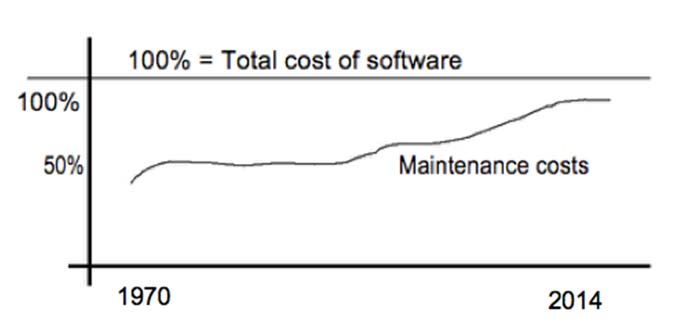
\includegraphics[width=0.7\linewidth]
				{./chapter-intro/img/software-maintence-costs}
\caption{Evolução da manutenção de software como percentual do custo total.
	Extraído de~\cite{engelbertink2010save}}
\label{fig:software-maintence-costs}
\end{figure}

Uma vez que o software entra em operação, anomalias são descobertas, mudanças
ocorrem no ambiente de operação e novos requisitos são solicitados pelo usuário.
Todas estas demandas devem ser solucionadas na fase de Manutenção que inicia
efetivamente com entrega do sistema, contudo, certas atividades ocorrem antes.

A \textit{Manutenção}, dentre outros aspectos, corresponde ao processo de
modificar um componente ou sistema de software após a sua entrega com o objetivo
de \textit{corrigir falhas, melhorar o desempenho ou adaptá-lo devido à mudanças
	ambientais}~\cite{{159342}}.  De maneira relacionada,
\textit{Manutenibilidade} é a propriedade de um sistema ou componente de
software em relação ao grau de \textit{facilidade} que ele pode ser corrigido,
melhorado ou adaptado~\cite{{159342}}.

Verificamos na literatura certa discussão sobre a diferença entre manutenção e
evolução de software.  Percebe-se ainda que pesquisadores e profissionais
utilizam evolução como substituto preferido para
manutenção~\cite{Bennett:2000:SME:336512.336534}. Todavia, não está no escopo
desta dissertação discutir e apresentar as diferenças entre os conceitos. Neste
sentido, utilizamos os termos \textit{manter} e \textit{evoluir} software de
forma intercambiáveis.

As manutenções em software podem ser divididas em \textit{Corretiva, Adaptativa,
	Perfectiva e Preventiva}~\cite{Lientz:1980:SMM:601062,159342}. A ISO 14764
discute os quatro tipos de manutenções, conforme já descrito, e além disso
propõe que exista um elemento comum denominado \textit{Requisição de Mudança}
que representa as características comuns a todas aqueles tipos de manutenção.

Por conta do volume das Requisições de Mudança se faz necessária a utilização de
ferramentas com o objetivo de gerenciá-las. Esse controle é geralmente realizado
por \textit{Ferramentas de Gerenciamento de Requisição de Mudança -~FGRM}, que
auxiliam os desenvolvedores na correção de forma individual ou colaborativa de
defeitos (bugs), no desenvolvimento de novas funcionalidades, dentre outras
tarefas relativas à manutenção de software.  A literatura não define uma
nomenclatura comum para este tipo de ferramenta. Em alguns estudos é possível
verificar nomes tais como Sistema de Controle de Defeito -~Bug Tracking Systems,
Sistema de Gerenciamento da Requisição -~Request Management System, Sistemas de
Controle de Demandas (SCD)- Issue Tracking Systems. Todavia, de modo geral, o
termo se refere as ferramentas utilizadas pelas organizações para \textit{gerir
	as Requisições de Mudança}. Estas ferramentas podem ainda ser utilizadas por
gestores, analistas de qualidade e usuários finais para atividades tais como
gerenciamento de projetos, comunicação, discussão e revisões de código. Neste
trabalho utilizaremos o termo \texttt{Ferramentas de Gerenciamento de
	Requisições de Mudança} (FGRM) ao referimos a este tipo de ferramenta.  A
Tabela~\ref{tab:exemplo} apresenta alguns exemplos de software que podem ser
classificadas como FGRM's. Também são listados serviços da Internet que oferecem
funcionalidades presentes nas FGRM na forma de Software como
Serviço~\cite{fox2013engineering}.

\begin{table}[ht]
	\centering
	\resizebox{\textwidth}{!}{%
		\begin{tabular}{llll}
			\hline
			\multicolumn{2}{c}{\textbf{Ferramentas}}           & \multicolumn{2}{c}{\textbf{Serviços da Internet}} \\ \hline
			Bugzilla & https://www.bugzilla.org/               & SourceForge    & https://sourceforge.net/    \\ \hline
			MantisBT & https://www.mantisbt.org/               & Lauchpad       & https://launchpad.net/      \\ \hline
			Trac     & https://trac.edgewall.org/              & Code Plex      & https://www.codeplex.com/   \\ \hline
			Redmine  & www.redmine.org/                        & Google Code    & https://code.google.com/    \\ \hline
			Jira     & https://www.atlassian.com/software/jira & GitHub         & https://github.com/         \\ \hline
		\end{tabular}%
	}
	\caption{Exemplos de ferramentas e serviços da Internet. Adaptado
		de~\cite{cavalcanti2014challenges}}\label{tab:exemplo}
\end{table}

\section{Motivação}
\label{sec:intro-motivacao}

\todo[inline]{O objetivo desta seção é apresentar a motivação do estudo. Em síntese, tenta responder
a seguinte pergunta: Por que dentro do contexto da manutenção de software estudar as Ferramentas de
Gerenciamento de Requisição de Mudança é IMPORTANTE?}

Diante da maior presença de software em todos os setores da sociedade existe um
interesse por parte da academia e da industria no desenvolvimento de processos,
técnicas e \textit{ferramentas} que reduzam o esforço e o custo das tarefas de
desenvolvimento e manutenção de software. Nesta linha, o trabalho de Yong \&
Mookerjee~\cite{1423995}  propõe um modelo que reduz os custos de manutenção e
reposição durante a vida útil de um sistema de software. O modelo demonstrou que
em algumas situações é \textit{melhor substituir um sistema do que mantê-lo}.
Este problema é agravado tendo em vista que o custo de manutenção que alguns
necessitam que 60\% dos desenvolvedores dedicados à tarefas de manutenção de
sistemas~\cite{Zhang_2003}.

Diversos projetos de software, especialmente durante as etapas de
desenvolvimento e teste do software, necessitam de uma ferramenta para gerenciar
as suas Requisições~de~Mudança tendo em vista o seu volume bem como pela grande
quantidade de pessoas inserir dados sobre os erros encontrados~\cite{1407819},
por exemplo. Este tipo de ferramenta vêm sendo utilizados em projetos de código
aberto (Apache, Linux, Open Office) bem como em organizações públicas e privadas
(NASA,IBM).

Não obstante, alguns estudos demonstram que as FGRM's desempenham um papel além
daquele de gerenciar os pedidos de manutenção e evolução do software. Avaliando
o controle de demandas como um processo social, Bertram et
al.~\cite{Bertram:2010:CCB:1718918.1718972} realizaram um estudo qualitativo em
FGRM's quando utilizados por pequenas equipes de desenvolvimento de software. Os
resultados mostraram que este tipo ferramenta não é apenas um banco de dados de
rastreamento de defeitos, recursos ou pedidos de informação, mas também atua
como um ponto focal para a comunicação e coordenação para diversas partes
interessadas (stakeholders) dentro e fora da equipe de software. Os clientes,
gerentes de projeto, o pessoal envolvido com a garantia da qualidade e
programadores, contribuem em conjunto para o conhecimento compartilhado dentro
do contexto das FGRM's.

No trabalho de Breu e outros~\cite{Breu:2010:INB:1718918.1718973} o foco é
analisar o papel dos FGRM's no suporte à colaboração entre desenvolvedores e
usuários de um software. A partir da análise quantitativa e qualitativa de
defeitos registrados em uma FGRM de dois projetos de software livre foi possível
verificar que o uso da ferramenta propiciou que os usuários desempenhassem um
papel além de simplesmente reportar uma falha: a participação ativa e permanente
dos usuários finais foi importante no progresso da resolução das falhas que eles
descreveram.

Um outro importante benefício da utilização das FGRM é que as mudanças no
software podem ser rapidamente identificada e reportada para os
desenvolvedores~\cite{anvik2005coping}. Além disso, eles podem ajudar a estimar
o custo do software, na análise de impacto, planejamento, rastreabilidade,
descoberta do conhecimento~\cite{cavalcanti2013bug}.

Nesta mesma linha, no contexto de utilização destas ferramentas diversos
desafios se apresentam: duplicação RM's, pedidos de modificação que são abertos
	inadvertidamente, grande quantidade de RM's que devem ser atribuídas aos
desenvolvedores, bugs descrito de forma incompleta, análise de impacto das RM's
e RM's atribuídas de maneira incorreta~\cite{cavalcanti2014challenges}.  Diante
de tantos problemas e desafios é importante entender como aquele tipo de
ferramente vêm sendo utilizada bem como analisar o que está sendo proposta na
literatura com objetivo de melhorar as funcionalidades oferecidas pelas FGRM\@.

%No trabalho de Junio et al.~\cite{5741246} é proposto um processo denominado
%PASM (Process for Arranging Software Maintenance Requests) que propõe lidar com
%tarefas de manutenção como projetos de software. Para tanto, utilizou-se
%técnicas de análise de agrupamento (clustering) a fim de melhor compreender e
%comparar as demandas de manutenção. Os resultados demostraram que depois de
%adotar o PASM os desenvolvedores tem dedicado um tempo maior para análise e
%validação. De outra forma, relacionada um menor tempo foi dedicado às tarefas
%de execução e codificação.
%
%No estudo realizado por Bettenburg et al.~\cite{bettenburg2008makes} foi
%desenvolvida uma pesquisa (\textit{survey}) entre desenvolvedores e usuários
%dos projetos Apache\footnote{\url{http://www.apache.org/}},
%Eclipse\footnote{\url{https://www.eclipse.org}} e
%Mozilla\footnote{\url{https://www.mozilla.org}} a fim de verificar o que
%produziria uma boa FGRM\@. Os resultados demonstraram que do ponto de vista dos
%desenvolvedores eram consideradas úteis funcionalidades tais como reprodução do
%erro, rastros de pilhas (stack traces) e casos de testes. A partir deste
%resultado foi construído um protótipo capaz de conduzir os usuários na coleta e
%fornecimento de um maior número de informações úteis para a resolução do
%defeito reportado.
%
%
%Em Zimmermann et al.~\cite{5070993} é discutido a importância de que a
%informação descrita em uma Requisição de Mudança seja relevante e completa a
%fim de que o defeito reportado seja resolvido rapidamente. Contudo, na prática,
%a informação apenas chega ao desenvolvedor com a qualidade requerida após
%diversas interações com o usuário afetado. Com o objetivo de minimizar este
%problema os autores propõe um conjunto de diretrizes para a construção de um
%ferramenta capaz de reunir informações relevantes a partir do usuário e
%identificar arquivos que precisam ser corrigidos para resolver o defeito.
%

%No trabalho de Kononenko et al.~\cite{Kononenko:2014:DED:2591062.2591075} é
%apresentada uma ferramenta denominada \textit{DASH} cujo objetivo é agrupar as
%demandas que são relevantes para as atividades de um desenvolvedor.
%Naturalmente todas as demandas ditas relevantes deveriam estar sob a
%responsabilidade de um mesmo programador. O principal objetivo desta ferramenta
%é aumentar a Consciência Situacional (Situational Awareness) dos
%desenvolvedores. Segundo os autores, o principal ganho do uso da ferramenta é
%que os programadores podem gerenciar melhor o excesso de informação e ficar
%mais ciente da evolução das demais demandas do sistema.
%
%Na ferramenta proposta por Thung et al.~\cite{Thung:2014:DIT:2642937.2648627} o
%foco é na determinação de defeitos duplicados. A contribuição deste trabalho é
%a integração do estado da arte de técnicas não supervisionadas para detecção de
%falhas duplicadas conforme proposto por Runeson et
%al.~\cite{Runeson:2007:DDD:1248820.1248882}. A ferramenta utiliza o Modelo de
%Vetor Espacial (Vetor Space Model) como métrica de similaridade entre os
%defeitos e fornece aos desenvolvedores uma lista de possíveis duplicatas.

%A manutenção não necessariamente exige que o processo de software envolvido
%seja o tradicional. Percebe-se alguns exemplos de adoção das práticas ágeis
%para fins de manutenção e evolução do software~\cite{kajko2009model,
%Heeager2015, Devulapally2015,Naz2016}. Tal tendência não é surpreendente tendo
%em vista que os métodos ``ágeis'' enfatizam características úteis à eficiência
%da implementação de software, tais como desenvolvimento incremental e teste
%contínuo que agregam valor para a evolução e manutenção eficaz de um sistema
%\cite{thomas2006agile}. Dentro desta tendência verifica-se a necessidade de que
%as ferramentas envolvidas no suporte à manutenção de software se adéquem à este
%nova forma de manter software.
%


\section{Problema}
\label{sec:intro-problema}

\todo[inline]{OBJETIVO\@: Apresentar o problema que esta dissertação pretende
	resolver. O problema deverá ser definido claramente ou deverão ser
	apresentadas provas da importância do mesmo dentro do escopo da Engenharia
	de Software}

O desenvolvimento e a manutenção de software envolvem diversos tipos de métodos,
técnicas e ferramentas. Em especial no processo de manutenção, um importante
aspecto são as diversas Requisições de Mudanças que devem ser gerenciadas. Este
controle é realizado pelas FGRM's cujo o uso vem crescendo em importância,
sobretudo, por sua utilização por gestores, analistas da qualidade e usuários
finais para atividades como tomada de decisão e comunicação. Contudo, muitas
daquelas ferramentas são meramente melhores interfaces para um banco de dados
que armazena todos os bugs reportados~\cite{zimmermann2009improving}.

Apesar da inegável importância das FGRM's, percebe-se um aparente desacoplamento
deste tipo de ferramenta com as necessidades das diversas partes interessadas
(stakeholders) na manutenção e evolução de software. A utilização de
\textit{``demanda''} como conceito central para Ferramentas de Gerenciamento de
Requisição de Mudanças (FGRM) parece ser distante das necessidades práticas dos
projetos de software, especialmente no ponto de vista dos desenvolvedores
\cite{Baysal:2013:SAP:2486788.2486957}.

Um exemplo deste desacoplamento deste tipo de ferramenta com a necessidade de
seus usuários pode ser visto no trabalho proposto por Baysal \&
Holme~\cite{baysal2012qualitative} no qual desenvolvedores que utilizam o
Bugzilla\footnote{\url{https://www.bugzilla.org}} relatam a dificuldade em
manter uma compreensão global das RM's em que eles estão envolvidos. Segundo os
desenvolvedores seria interessante que a ferramenta tivesse um suporte melhorado
para a Consciência Situacional -~Situational Awareness. Em síntese, eles
gostariam de estar cientes da situação global do projeto bem como das atividades
que outras pessoas estão realizando.

Um outro problema que é potencializado pela ausência de certas funcionalidades
nas FGRM são as RM's que acabam sendo relatadas de forma insatisfatória. Nesta
situação os usuários acabam sendo questionados a inserir maiores detalhes que
muitas vezes eles não tem conhecimento. Por outro lado, verifica-se uma
frustração por parte dos desenvolvedores que acabam desapontados sobre a
qualidade do que foi reportado~\cite{just2008towards}.

Com o objetivo de melhorar as FGRM, que no contexto do trabalho recebem o nome
de issue tracking system, Zimmermann e outros
discute~\cite{zimmermann2009improving} quatro dimensões de melhorias deste tipo
de ferramenta, conforme esquematizado na
Figura~\ref{fig:dimensoes_melhorias_fgrm}:

\begin{description}
	\item[Informação] Estas melhorias focam diretamente na informação fornecida
		pelo reportador da RM\@. Com ajuda da FGRM o responsável por descreve um
		bug, por exemplo, poderia ser motivado a coletar mais informações sobre o
		problema. O sistema poderia verificar a validade e consistência daquilo
		que foi repassado pelo usuário.
   \item[Processo] Melhorias com foco no processo visam dar suporte à
	   administração de atividades relacionadas à solução de RM\@. Por exemplo, a
	   triagem de RM, poderia ser automatizada visando acelerar o processo. Um
	   outro exemplo de melhoria poderia ocorrer no aumento do entendimento do
	   progresso realizado em cada RM ou mesmo fornecer ao usuário afetado uma
	   estimativa de em quanto tempo a sua requisição será solucionada. 
	\item[Usuário] Nesta dimensão estão incluídos tanto os usuário que relatam
		as RM's quanto os desenvolvedores responsável por solucioná-la. Os
		reportadores podem ser educados de qual informação fornecer e como
		coletá-la. Os desenvolvedores também podem beneficiar de um treinamento
		similar em qual informação esperar e como esta informação pode ser
		utilizada para solucionar a RM\@.
	\item[Ferramenta] As melhorias centradas na ferramenta são realizadas nas
		funcionalidades fornecidas pelas FGRM\@. Elas podem reduzir a complexidade
		da coleta e fornecimento das informações necessárias para solucionar o
		RM\@. Por exemplo, as FGRM poderiam ser configuradas para automática
		localizar a pilha de erro (stack trace) e adicioná-la ao erro reportado.
		A ferramenta poderia simplificar o processo de reprodução do erro
		mediante a simplificação do processo de capturas de telas. Estes
		exemplos visam ajudar com a coleta das informações necessárias pelos
		desenvolvedores para corrigir o bug, por exemplo.
\end{description}

\begin{figure}[htpb] \centering
	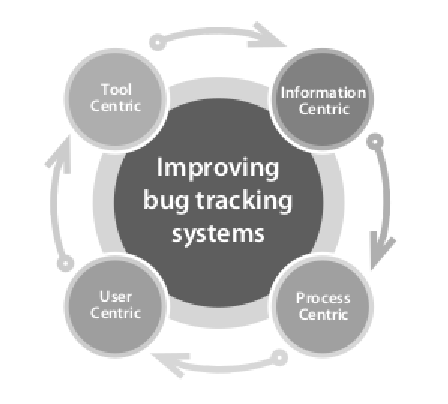
\includegraphics[width=0.666666\linewidth]
	{chapter-intro/img/dimensoes_melhorias_fgrm.pdf}
	\caption{Dimensões de melhoria das FGRM's. Adaptado
		de~\cite{zimmermann2005mining}}\label{fig:dimensoes_melhorias_fgrm}
\end{figure}

Neste estudo estamos especialmente interessados em analisar e propor melhorias
relativas ao domínio da \textit{Ferramenta}. Ao bem do nosso conhecimento é
reduzido o número de trabalhos que avaliem de forma sistemática as
funcionalidades oferecidas pelas FGRM ao mesmo tempo que faça relação com que
vêm sendo proposto na literatura sobre o assunto. De maneira similar é reduzido
o número de estudo que avaliam a opinião dos profissionais envolvidos em
manutenção de software sobre o que é ofertado pelas FGRM\@.

Além disso, os estudos anteriormente propostos não discutem o fato que da mesma
forma que ocorre no desenvolvimento de software, é possível verificar uma
crescente adoção de técnicas da metodologia ágil na manutenção de
software~\cite{Soltan2016,Devulapally2015, Heeager2015}. Neste contexto, seria
importante que ferramentas que dão suporte à manutenção, tal como as FGRM's,
evoluíssem para se adaptar a esta nova forma de trabalhar. Mesmo em um
ambiente tradicional de  desenvolvimento e manutenção de software, verifica-se a
necessidade de adequação das FGRM's, o que pode ser observado considerando as
diversas extensões (plugins) propostas na literatura
\cite{101186,Thung:2014:BIT:2635868.2661678,Kononenko:2014:DED:2591062.2591075}.

\section{Objetivos}
\label{sec:intro-objetivos}

Conforme exposto o distanciamento entre as necessidades dos profissionais
envolvidos em manutenção de software e as funcionalidades oferecidas pelas FGRM
resulta em diversos problemas. Neste contexto, este trabalho de dissertação
investiga e contribui no entendimento de como as Ferramentas de Gerenciamento de
Requisição de Mudança estão sendo melhoradas ou estendidas no contexto da
transformação do processo de desenvolvimento e manutenção de software de um
modelo tradicional para outro que incorpora cada vez mais as práticas propostas
pelos agilistas. O intuito foi analisar como as FGRM estão sendo modificadas com
base na literatura da área em contraste com o ponto de vista dos profissionais
envolvidos em manutenção de software.

Neste contexto, elaboramos um estudo das Ferramentas de Gerenciamento de
Requisição de Mudança (FGRM) com os seguintes objetivos:
\begin{enumerate}[(i)]
	\item entender os requisitos comuns deste tipo de ferramenta;
	\item mapear as extensões para as FGRM que estão sendo propostas na
		literatura;
	\item avaliar sobre o ponto de vista dos profissionais a
		situação atual dos FGRM\@;
	\item propor melhorias ou novas funcionalidades para as FGRM\@. 
\end{enumerate}

%Vamos discutir os aspectos que são considerados mais importantes a partir da
%literatura da área, bem como do ponto de vista de profissionais envolvidos em
%manutenção de software. De forma particular, iremos estudar os mecanismos de
%personalização que algumas destas ferramentas permitem e tentaremos ainda criar
%exemplos de personalização para alguma possível extensão a ser identificada ao
%longo do trabalho.

\section{Visão Geral do Estudo}
\label{sec:intro-visao-geral}

\todo[inline]{OBJETIVO\@: Apresentar de forma sucinta o trabalho realizado nesta
	dissertação com o objetivo de apresentar uma solução para o problema
	declarado na seção anterior.}

A fim de alcançarmos os objetivos descritos na seção anterior, um conjunto de
melhorias nas funcionalidades das FGRM's foi proposto. As melhorias propostas
são o resultado de três estudos empíricos: um mapeamento sistemático da
literatura, apresentado no Capítulo~\ref{ch:mapeamento-sistematico}, uma
caracterização das funcionalidades das FGRM, discutida no
Capítulo~\ref{ch:caracterizacao}; e uma pesquisa com profissionais, apresentada
no Capítulo~\ref{ch:pesquisa-profissionais}.

Mediante o mapeamento sistemático foi possível obter e avaliar o estado da arte
sobre novas funcionalidades bem como melhorias no escopo das FGRM\@. A partir do
estudo foi possível propor quatro esquemas de classificação: por tipo de
problema, por suporte ao papel da manutenção de software, por técnicas de
Recuperação da Informação utilizada e por ferramenta estendida.\todo{A medida
	que o mapeamento for concluído irei adicionar os resultados obtidos.}

De maneira similar, através da caracterização das funcionalidade de algumas de
código aberto ou disponíveis comercialmente identificamos o estado da prática
deste tipo de ferramenta.\todo{Incluir os resultados da caracterização das
	ferramentas de forma sucinta.}

Com base dois estudos anteriores conduzimos uma pesquisa com
profissionais envolvidos em manutenção de software onde pedimos que avaliassem
os requisitos funcionais e não funcionais que poderiam melhorar as FGRM já
existentes. O questionário também quis saber a opinião dos profissionais sobre a
relevância das propostas de melhorias existente na literatura em sua
rotina.\todo{Incluir os resultado de forma sucinta da pesquisa com profissionais}

\section{Metodologia de Pesquisa}
\label{sec:intro-metodologia}
\todo[inline]{OBJETIVO\@: Em linhas gerais apresenta como o problema descrito na
	seção anterior foi resolvido mediante a apresentação da metodologia
	científica utilizada}

A metodologia de pesquisa utilizada neste estudo é baseada em uma abordagem
multi-método~\cite{hesse2010mixed}. Este tipo de desenho de pesquisa combina
dois ou mais métodos quantitativo ou qualitativo em um único estudo. Um estudo
que faça uso de um survey e um experimento é um exemplo deste tipo de
enfoque~\cite{hesse2010mixed}.

Alguns estudos descrevem quatro tipos de desenho em abordagens multi-método:
embutida (embedded), exploratória, triangulada e
explanatória~\cite{creswell2007designing}. Neste estudo, utilizamos uma
abordagem de triangulação no qual consolidamos os resultados de diferentes
métodos, considerando, contudo, que a mesma questão de pesquisa foi investigada
em cada um deles. A utilização de um desenho triangular no trabalho melhora as
conclusões e completude do estudo, trazendo maior credibilidade para os achados
da pesquisa~\cite{hesse2010mixed}

As etapas do trabalho, que compõem a abordagem multi-método estão listadas a seguir:

\begin{itemize}[(i)]
	\item Mapeamento Sistemático da Literatura~\cite{keele2007guidelines}
	\item Caracterização das Ferramentas de Gerenciamento de Requisição de Mudança (FGRM)
	\item Pesquisa (Survey) com os desenvolvedores~\cite{wohlin2012experimentation}
%	\item Desenvolvimento de extensões para as FGRM's
\end{itemize}

\section{Contribuições do Estudo}
\label{sec:intro-contribuicao}
\todo[inline]{Aguardar o andamento do estudo para melhor discutir as
	contribuição efetivas do mesmo}
\section{Organização do Trabalho}
\label{sec:intro-organizacao-dissertacao}
\todo[inline]{Vamos aguardar o desenvolvimento deste trabalho para definirmos a
estrutura do texto.}


%Incluindo o fonte do Capítulo 02
%%%%%%%%%%%%%%%%%%%%%%%%%%%%%%%%%%%%%%%%%%%%%%%%%%%%%%%%%%%%%%%%%%%%%%%%%%%%%%%%
%Objetivo: Descrever os principais conceitos relativos a Manutenção de Software
%		   envolvidos na dissertação
%Autores: Vagner Clementino <vagnercs@dcc.ufmg.br>
%		  Rodolfo Resende <rodolfo@dcc.ufmg.br>
%Criação: Ter Set 13 19:22:37 BRT 2016
%Modificação: Dom Set 25 15:53:04 BRT 2016
%Revisão:  Ter Set 20 19:13:49 BRT 2016
%%%%%%%%%%%%%%%%%%%%%%%%%%%%%%%%%%%%%%%%%%%%%%%%%%%%%%%%%%%%%%%%%%%%%%%%%%%%%%%%

\chapter{Manutenção de Software: Uma Visão Geral}
\label{ch:visao-geral-manutencao}

Uma tendência natural do software é evoluir a fim de atender aos novos
requisitos e alterações do ambiente no qual ele está inserido. Em uma série de
estudos, Lehman propõe um conjunto de leis sobre a evolução do software. Dentre
elas podemos destacar as leis da Mudança Contínua (Continuing Change) e da
Complexidade Crescente (Increasing complexity). A primeira diz que um programa
que é utilizado em um ambiente real deve mudar ou se tornará progressivamente
menos útil~\cite{lehman1980understanding}. A lei da Complexidade Crescente
(Increasing complexity) afirma que quando um sistema em evolução muda, sua
estrutura tende a se tornar mais complexa. Nesta situação, recursos extras devem
ser disponibilizados a fim de preservar e simplificar a estrutura do
software~\cite{lehman1980understanding}. As leis de Lehman tem sido validadas,
especialmente aquelas relacionadas a tamanho e complexidade do software. Em um
trabalho sobre o tema Yu \& Mishra~\cite{{yu2013empirical}} examinaram de forma
empírica as Leis de Lehman em relação a evolução da qualidade do software. O
estudo demonstrou que com base na métrica proposta que a qualidade de um produto
de software declinará ao menos que uma restruturação é realizada.

Conforme exposto, a mudança em um produto de software é inevitável. Desta forma,
é importante a existência de uma área de estudo preocupada com o gerenciamento e
controle destas mudanças. Dentro do escopo da Engenharia de Software esta tarefa
fica a cargo da Manutenção de Software.  Nas próximas seções discutimos os
conceitos básicos que mostram onde e como a Manutenção se encaixa dentro da
Engenharia de Software. São apresentados os conceitos que fazem da Manutenção de
Software uma disciplina distinta.

%Percebida a importância do processo de manutenção de software, alguns trabalhos
%foram propostos visando mensurar o seu custo bem como propor processos com o
%objetivo de reduzir o esforço envolvido neste tipo de atividade.
%
%No trabalho de Herrin~\cite{Herrin:1985:SMC:323287.323383} foi proposto um
%modelo matemático com o objetivo de avaliar o impacto financeiro no orçamento
%de uma universidade devido às atividades de manutenção no sistema de
%processamento de dados da instituição. O modelo propõe que o valor disponível
%para desenvolvimento de um novo sistema é função inversa do custo de manutenção
%do software existente. Desta forma, o fato de se manter um sistema durante
%muito tempo poderá impossibilitar a aquisição ou mesmo o desenvolvimento de um
%novo.
%
%No estudo de Hirota et al.~\cite{hirota1994approach} é proposta a utilização da
%técnica Análise de Ripple para estimar o custo da manutenção de software. O
%termo ``efeito Ripple'' foi utilizado pela primeira vez em um artigo publicado
%por Haney~\cite{haney1972module} para descrever a forma que a mudança em um
%módulo poderia causar alterações em outras partes do
%sistema~\cite{bilal2005using}. A Análise Ripple é, portanto, uma técnica para
%analisar o fluxo de dados de variáveis dentro de um determinado programa. Os
%valores retornados pela aplicação do método são denominados Complexidade de
%Ripple. Os resultados demostraram que a Complexidade de Ripple está mais
%relacionada ao entendimento do software do que as métricas padrão, como linhas
%de código, complexidade ciclomática e pontos de função. Desta forma, a
%Complexidade de Ripple poderia ser utilizada, por exemplo, para predizer os
%custo de manutenção de um sistema, bem como a necessidade de substituição do
%mesmo.
%
%Mediante o uso de Redes Neurais Shula \& Misra
%\cite{Shukla:2008:ESM:1342211.1342232} propõe um estudo para medir o custo de
%manutenção de software. O trabalho discute a utilização de outras métricas além
%de linha de código e pontos de função para medir  tamanho e custo do processo
%de manutenção. Os resultados demonstraram a possibilidade de construir um
%modelo para medir o custo utilizando Redes Neurais. Contudo, os resultados são
%sensíveis a escolha da arquitetura e parâmetros de treino, os quais idealmente
%deveriam ser preparados por um especialista no sistema (oráculo).
%
%A dinamicidade do ambiente de negócios tem levado a diversas organizações a
%adotar as metodologias propostas pelos agilistas pelo fato delas auxiliarem no
%atendimento das exigências do cliente~\cite{Devulapally2015}. Esta tendência é
%mais forte no desenvolvimento de software e nos últimos anos vem ocorrendo de
%forma gradativa na manutenção.
%
%No trabalho de Kajko-Mattsson \& Nyfjord~\cite{4755767} foi proposto um modelo
%ágil para manutenção que apropria diferentes práticas do Extreme Programming e
%do Scrum. Segundo os autores a junção desta duas metodologias possibilita a
%inclusão de práticas úteis tanto do ponto de vista do gerente do projeto bem
%como dos desenvolvedores. O modelo encoraja diversas práticas tais como
%\textit{product backlog}, testes antes da codificação, planejamento iterativo,
%dentre outras.
%
%A adoção na manutenção de software de algumas práticas propostas pelos
%agilistas foram analisadas durante 08 meses em estudo realizado por Svensson \&
%Host~\cite{1402140}. Ao utilizar o Extreme Programming (XP) no processo de
%manutenção os autores concluíram que é muito difícil fazer uso do XP sem que
%sejam realizadas adequações no desenho de diversas práticas para desta forma
%adequar às necessidades do time de desenvolvimento.
%
%O estudo Heeager \& Rose~\cite{Heeager2015} propõe um conjunto de nove
%heurísticas com o objetivo de ajudar aos profissionais da manutenção de
%software na adoção de práticas propostas pelos agilistas. O trabalho consistiu
%da inclusão do Scrum na rotina de trabalho do departamento de manutenção de
%software de uma organização de grande porte. Os autores argumentam que os
%métodos ágeis, quando aplicado ao trabalho de desenvolvimento, têm certas
%características relativamente bem compreendidas, no entanto o trabalho de
%manutenção difere do de desenvolvimento em certos aspectos e, portanto, é
%desafiador a implementação de métodos ágeis em um departamento de manutenção.
%
\section{Conceitos Fundamentais}
\label{sec:conceitos_basicos}

Esta seção introduz os conceitos e terminologias que ajudam no entendimento do
papel e escopo da Manutenção de Software. De uma maneira geral, podemos definir
atividade de manter software como a totalidade das ações necessárias para
fornecer suporte a um produto de software. Entretanto, encontramos na literatura
outras definições mais elaboradas sobre a área.

Manutenção de Software é definida pela IEEE 1219~\cite{ISO-1219-1998}-~Padrão para a
Manutenção de Software, como a modificação de um produto de software após a sua
entrega com o objetivo de corrigir falhas, melhorar o desempenho ou outros
atributos com a finalidade de adaptar o software as modificações ambientais. O
padrão cita a ocorrência de atividade de manutenção antes da entrega
propriamente dita, contudo, de forma bastante superficial.

Posteriormente a IEEE/EIA 12207~-~Padrão para o Processo de Ciclo de Vida do
Software~\cite{{ISO/IEC-12207-2008}} retrata a manutenção como um dos principais processos no
ciclo de vida do software. Em seu texto a manutenção é vista como atividade de
modificação do código e da documentação associada e ocorre devido a algum
problema ou necessidade de melhoria~\cite{IEEEComputerSociety:2014:GSE:2616205}.
Por outro lado a ISO/IEC 14764~-~Padrão para Manutenção de
Software~\cite{1703974}enfatiza aspectos pré-entrega da manutenção, como por
exemplo o planejamento.

De maneira relacionada, \textit{Manutenibilidade} é a propriedade de um sistema
ou componente de software em relação ao grau de \textit{facilidade} que ele pode
ser corrigido, melhorado ou adaptado~\cite{{159342}}. A
ISO/IEC~9126~-~01~\cite{ISOIEC9126} define a Manutenibilidade como uma
característica de qualidade do processo de Manutenção.

Apesar das diversas definições para Manutenção de Software é possível
identificar dois aspectos comuns: manter e evoluir. O conceito de evolução de
software carece de uma definição padrão na literatura, contudo, pesquisadores e
profissionais utilizam o termo como substituto preferido para
manutenção~\cite{Bennett:2000:SME:336512.336534}. Embora exista o entendimento
que os processos de manutenção e evolução possuem características distintas, não
está no escopo desta dissertação discutir e apresentar tais diferenças. Neste
sentido, utilizamos os termos \textit{manter} e \textit{evoluir} software de
forma intercambiáveis. Caso em algum contexto haja a necessidade de
diferenciação, ela será discutida.

A Manutenção é necessária para garantir que o software seja capaz de satisfazer
os requisitos dos usuários. Neste sentido, a atividade de manter software pode
ser vista como um desenvolvimento contínuo, sobretudo, pelo fato que alguns
sistemas nunca estão completos e continuam a evoluir.

\section{Requisição de Mudança}
\label{sec:requisição_de_mudanca}

As manutenções em software podem ser divididas em \textit{Corretiva, Adaptativa,
	Perfectiva e Preventiva}~\cite{Lientz:1980:SMM:601062,159342}.  A Manutenção
Corretiva lida com a reparação de falhas encontradas. A Adaptativa tem o foco na
adequação do software devido à mudanças ocorridas no ambiente em que ele está
inserido. A Perfectiva trabalha para detectar e corrigir falhas latentes. A
Preventiva preocupa com atividades que possibilitem aumento da manutenibilidade
do sistema.  A \textit{ISO 14764}~\cite{1703974} propõe a divisão da tarefa de
manutenção nos quatro tipos descritos anteriormente e propõe que exista um
elemento comum denominado Requisição de Mudança que representa as
características comuns a todas aqueles tipos de manutenção.o A
Figura~\ref{fig:modification-request} exibe a classificação das RM's conforme
discutido pela ISO\@.

\begin{figure}[hbtp] \centering 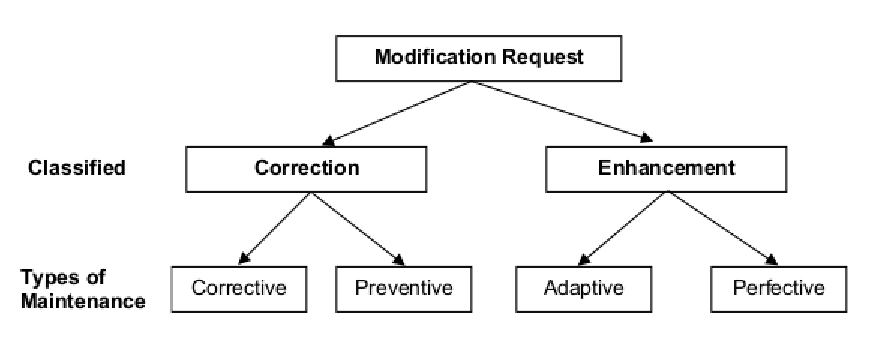
\includegraphics[width=.75\textwidth]
	{chapter-intro/img/modification_request.eps} \caption{Tipos de manutenção
		segundo a norma ISO/IEC 14764. Extraído de~\cite{1703974}}
	\label{fig:modification-request} \end{figure}

A ISO/IEC 14764 classifica as manutenções adaptativas e perfectivas como
melhorias e agrupa as manutenções corretivas e preventivas em uma única
categoria de correção, conforme exibido na
Tabela~\ref{tab:categorias_requisicao_mudanca}. A manutenção preventiva é mais
frequentemente realizada em produtos de software onde atributos de segurança são
mais críticos.
%At Modification requests are logged and tracked, the impact of proposed changes
%is determined, code and other software artifacts are modified, testing is
%conducted, and a new version of the software product is released

\begin{table}[htpb] \centering 	\begin{tabular}{l|l|l|} \cline{2-3} &
		\textbf{Correção} & \textbf{Melhoria} \\ \hline
		\multicolumn{1}{|l|}{\textbf{Pró-ativa}} & Preventiva & Perfectiva \\
		\hline \multicolumn{1}{|l|}{\textbf{Reativa}} & Corretiva & Adaptativa
		\\ \hline \end{tabular}\caption{Categorias da Requisição de Mudanças.
		Adaptado de
		SWEBOK~\cite{4425813}}\label{tab:categorias_requisicao_mudanca}
\end{table}

Em síntese, apesar das diferentes nomenclaturas existentes na literatura
(demanda, bug, defeito, bilhete, tíquete, requisição de modificação, relato de
problema) uma Requisição de Mudança representa o relato, independente de sua
estrutura, que têm por objetivo gerar a manutenção ou evolução do software.

\section{O processo de Manutenção de Software}
\label{sec:o_processo_de_manutecao_de_software}

Um Processo de Software é o conjunto de atividades, métodos, práticas e
transformações utilizadas para desenvolvê-lo ou mantê-lo bem como seus artefatos
associados~\cite{paulk1993key}. Independente do contexto em que a manutenção
ocorra é importante que o processo esteja bem definido. Existe na literatura a
proposição de alguns modelos do processo de manutenção de software,
especialmente baseado em uma visão tradicional no qual desenvolvimento e
manutenção possuem uma clara separação. Recentemente os métodos propostos pelos
agilistas vêm sendo utilizados para manter software. Esta tendência surge da
demanda crescente por serviços de manutenção com um retorno mais rápido para o
usuário.

Nas próximas seções apresentamos alguns modelos encontrados na literatura na
perspectiva tradicional, ao mesmo tempo descrevemos propostas do uso da
metodologia dos agilistas na manutenção de software.

\subsection{Manutenção de Software Tradicional}
\label{subsec:manutenção_de_software_tradicional}

Em resumo, um processo de manutenção de software descreve as atividades e suas
respectivas entradas e saídas. Alguns modelos são descritos nos padrões IEEE
1219 e ISO/IEC 14764. O processo especificado no Padrão para Manutenção de
Software (IEEE-~1219) indica que as atividade de manutenção de software iniciem
após a entrega do produto de software. O padrão também discute itens para fins
de planejamento da manutenção. As atividades que compõe o processo são
apresentas na Figura~\ref{fig:ieee-1219-processo-man-software}.

\begin{figure}[htpb] \centering
	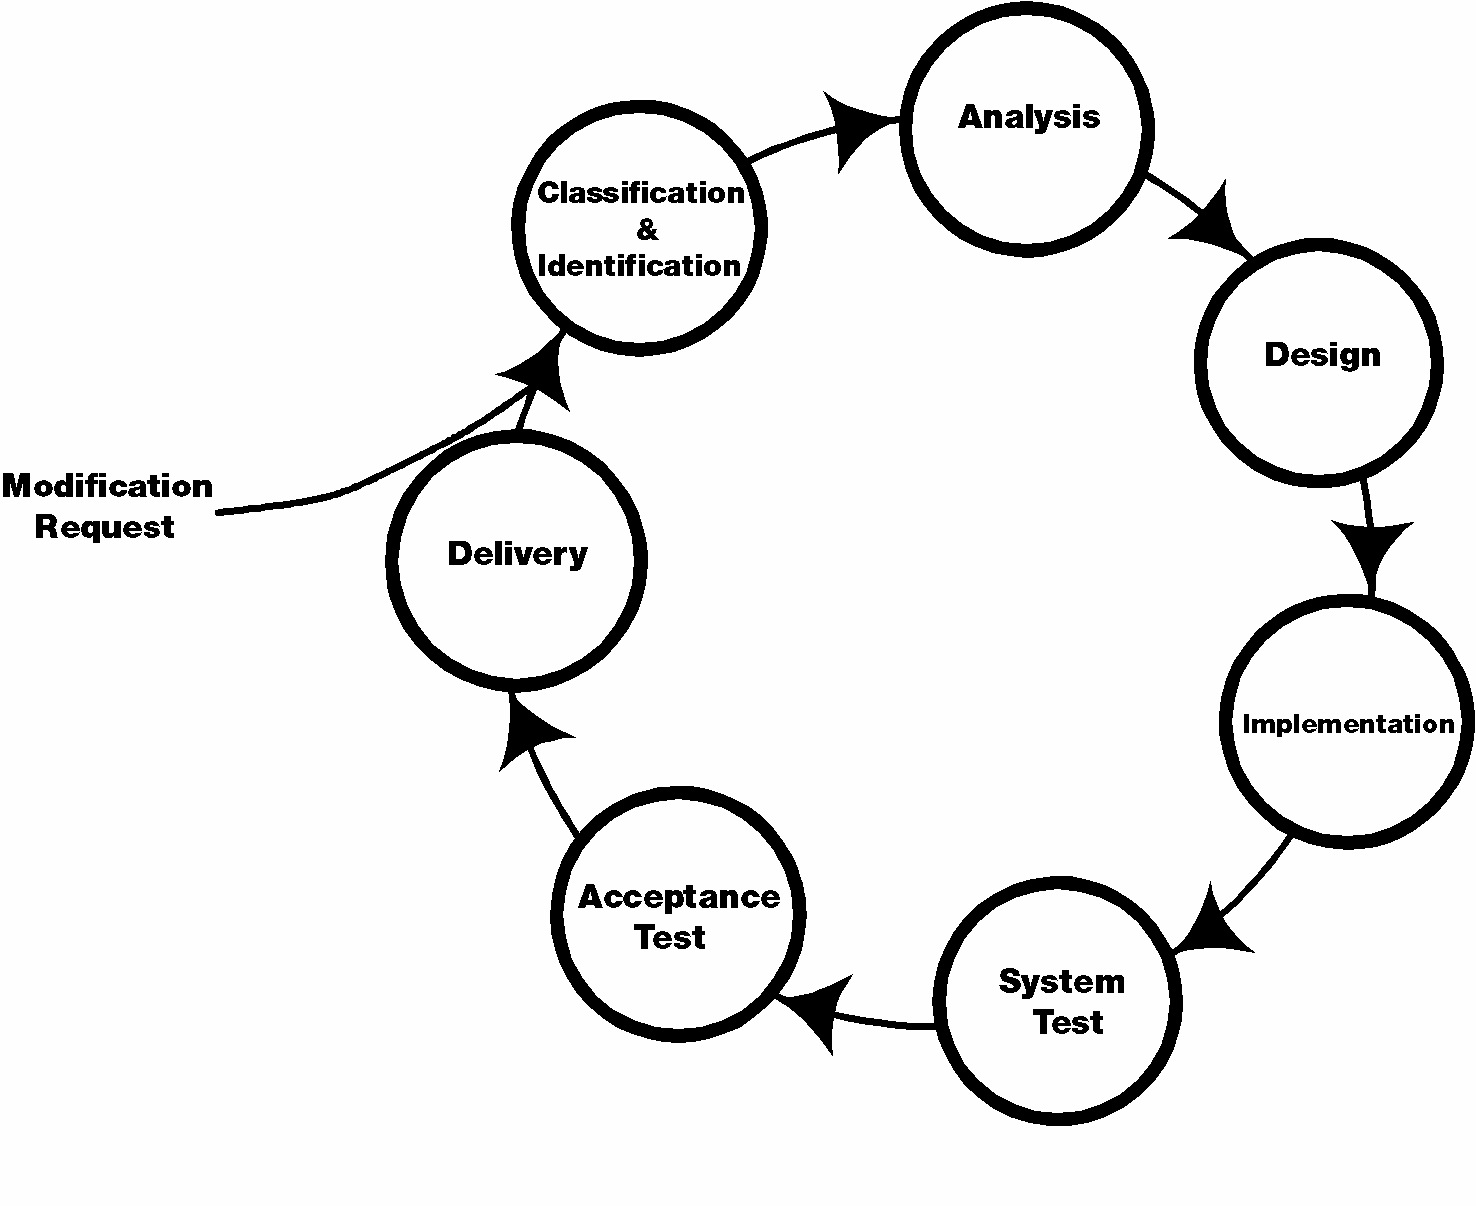
\includegraphics[width=0.7\linewidth]
	{chapter-manutencao-software-visao-geral/img/ieee-1219-98-processo-manutencao.png}
	\caption{IEEE 1219 -~Processo de Manutenção de Software}\label{fig:ieee-1219-processo-man-software}
\end{figure}

De maneira relacionada, na ISO/IEC 14764 as atividades que compõe o processo são
similares aquelas propostas na IEEE-~1219, exceto pelo fato que elas são
agregadas de uma forma diferente. O processo descrito na ISO/IEC~14764 são
exibidas na Figura~\ref{fig:ieee-14764-processo-manutencao}

\begin{figure}[htpb] \centering
	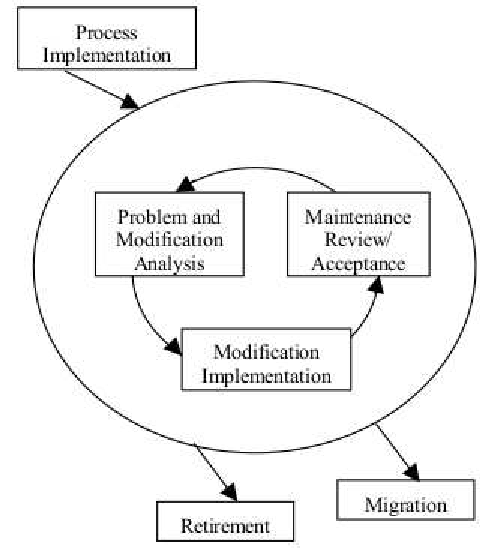
\includegraphics[width=0.7\linewidth]
{chapter-manutencao-software-visao-geral/img/ieee-14764-processo-manutencao.pdf}
	\caption{ISO/IEC~14764 Processo de Manutenção de Software}
\label{fig:ieee-14764-processo-manutencao} \end{figure}

As atividades de manutenção propostas na ISO/IEC 14764 são detalhadas em tarefas
conforme apresentadas a seguir:

\begin{itemize} \item Implementação do Processo \item Análise e Modificação do
		Problema \item Aceitação e Revisão da Manutenção \item Migração \item
		Aposentadoria do Software	\end{itemize}

É possível notar que algumas atividades realizadas durante a manutenção de
software são similares a a outras presentes no desenvolvimento de software, como
por exemplo, análise de desempenho, codificação, teste e documentação. Outra
atividade comum à manter e desenvolver software é o gerenciamento dos
requisitos. Nas duas situações os profissionais responsáveis por controlar os
requisitos devem atualizar documentação  por conta de alterações ocorridas no
código fonte. Por outro lado certas atividades estão vinculadas apenas ao
contexto da manutenção de software. Dentre elas podemos destacar:

\begin{description}
	\item[Suporte ao Usuário] Função de ajuda ao usuário final
		que podem disparar ações tais como avaliação e priorização das
		Requisições de Mudanças
   	\item [Análise de Impacto] \todo{Descreve melhor
			análise de impacto}
   	\item [Suporte ao Uso de Software] Ajuda aos
		usuários final com relação a determinada requisição de informação
		(regras de negócio, validação e requisição de relatório)
	\item [Acordo de Nível de Serviço] Definição de um nível mínimo de qualidade que a
		atividade de manutenção deve ser realizada.
\end{description}

\subsection{Manutenção de Software com Método dos Agilistas}
\label{sub:manutenção_de_software_com_método_dos_agilistas}

Grande parte da literatura de manutenção de software trata de técnicas e
metodologias tradicionais da Engenharia de Software. Entretanto, é possível
verificar um protagonismo das práticas propostas pelos agilistas em projetos de
sucesso, mesmo em áreas não relativas à Tecnologia da
Informação~\cite{Serrador2015}. Neste contexto, verifica-se uma tendência que os
departamentos dedicados à manutenção de software se mostrem interessados nas
metodologias dos agilistas e que tenham vontade de experimentá-las em suas
atividades~\cite{Heeager2015}.

Apesar da maioria dos textos em Engenharia de Software tratarem desenvolvimento
e manutenção como atividades com natureza distintas, esta última pode adaptar
características da primeira visando a melhoria do seu desempenho. Dentre as
práticas propostas pelos agilistas passíveis de serem utilizadas em tarefas de
manutenção é possível citar o desenvolvimento iterativo, maior envolvimento do
cliente, comunicação face a face, testes frequentes, dentre outras.

Alguns resultados demonstram certa dificuldade para implantação da metodologia
dos agilista na manutenção de software~\cite{1402140}. Um dos possíveis
problemas é a necessidade de adequação das práticas da organização de modo que a
se adequar as necessidades do time de desenvolvimento.  Estudo apresentam
resultados relativos à melhorias no aprendizado e produtividade da equipe
mediante o aumento da moral, encorajamento e confiança entre os desenvolvedores,
o que propicia uma alta motivação durante o processo de manutenção de
software~\cite{Choudhari:2014:EIM:2557833.2557845}.

\section{Ferramentas de Gerenciamento de Requisições de Mudança (FGRM)}
\label{sec:ferramentas_de_gerenciameto_de_requisições_de_mudança}

Dentro da disciplina de Gerenciamento da Configuração do Software a atividade de
controle de configuração é responsável por gerenciar mudanças ocorridas durante
o ciclo de vida de um produto de software. Tais ações incluem determinar quais
alterações serão feitas, definir a autoridade responsável por autorizar certos
tipos de mudança e aprovar desvios relativos aos requisitos iniciais do
projeto~\cite{4425813}. De uma forma mais ou menos estruturada este tipo de
processo ocorre em diferente tipos de projeto de software, seja ele dentro de um
processo de manutenção tradicional ou mesmo naqueles que utilizam os métodos
propostos pelos agilistas.

Por conta do volume das Requisições de Mudança se faz necessária a utilização de
ferramentas com o objetivo de gerenciá-las. Esse controle é geralmente realizado
por Sistemas de Controle de Demandas (SCD)- Issue Tracking Systems, que auxiliam
os desenvolvedores na correção de forma individual ou colaborativa de defeitos
(bugs), no desenvolvimento de novas funcionalidades, dentre outras tarefas
relativas à manutenção de software. Não existe na literatura uma nomenclatura
comum para este tipo de ferramenta. Em alguns estudos é possível verificar nomes
tais como Sistema de Controle de Defeito\@-\@ Bug Tracking Systems, Sistema de
Gerenciamento da Requisição\@-\@ Request Management System, Sistemas de Controle de
Demandas (SCD)- Issue Tracking Systems e diversos nomes afins. Todavia, de modo
geral, o termo se refere as ferramentas utilizadas pelas organizações para
\textit{gerir as Requisições de Mudança}. Estas ferramentas podem ainda ser
utilizadas por gestores, analistas de qualidade e usuários finais para
atividades tais como gerenciamento de projetos, comunicação, discussão e
revisões de código. Neste trabalho utilizaremos o termo \texttt{Ferramentas de
	Gerenciamento de Requisições de Mudança} (FGRM) ao referimos a este tipo de
ferramenta.

No últimos anos alguns estudos discutem o fato que as FGRM's não apenas ajudam
as organizações gerenciar, atribuir, controlar, resolver e arquivar Requisições
de Mudança. Em alguns casos, este tipo de ferramenta se tornou o ponto focal
para comunicação e coordenação para diversas partes interessadas, dentro e além
da equipe de manutenção~\cite{Bertram:2010:CCB:1718918.1718972}.  As FGRM's
também servem como um repositório central para monitorar o progresso da RM,
solicitar informações adicionais da pessoa responsável por redigir a requisição
e o ponto de discussão para potenciais soluções um
bug~\cite{zimmermann2009improving}.

Em projetos de código aberto, as FGRM são uma importante parte de como o time
interage com comunidade de usuários. Como consequência é possível observar o
fenômeno da participação dos usuários no processo de solução da RM:\@ eles não
apenas submetem a RM, mas também participam na discussão de como resolvê-la.
Desta forma, o usuário final ajuda tomar as decisões sobre a direção futura do
produto de software~\cite{breu2010information}.

Conforme exposto as FGRM desempenham um papel que vai além de gerenciar as
Requisições de Mudança.  Neste sentido, é importante estudar este tipo de
software em busca de como melhorá-las de modo a atender as diversas necessidades
dos seus usuários. Contudo, é importante avaliar as novas funcionalidades
propostas na literatura ou ainda mesmo a melhoria das já existentes. Uma
possível forma de melhoria é através do uso de extensões. Na próxima seção
discutiremos esta propriedade de algumas FGRM's que permitem a inclusão e
modificação de funcionalidades e comportamentos da ferramenta segundo as
necessidades do usuário.

\subsection{Extensões em FGRM}
\label{subsec:extensoes_fgrm}

Em determinados domínios de aplicação é interessante desenvolver produtos de
software com uma arquitetura que permita o sistema se adaptar às mudanças nos
requisitos. Existe naturalmente a possibilidade de incluir as novas
funcionalidades dentro das já existentes no software, todavia, verificamos que
sistemas que permitem extensões apresentam os seguintes benefícios:

\begin{itemize} \item Extensibilidade: o software pode se dinamicamente
		estendido mediante a inclusão de novas características.  \item
		Desenvolvimento em Paralelo: Desde de que as funcionalidades podem ser
		implementadas como componentes separados, eles podem ser desenvolvidos
		em paralelo por times diferentes \item Simplicidade: uma  extensão
		tipicamente tem uma única funcionalidade, desta forma os desenvolvedores
		possuem o único foco.  \end{itemize}

No escopo deste trabalho, uma extensão é um componente de software que adiciona
uma característica ou comportamento específico para um programa de
computador\footnote{\url{https://en.wikipedia.org/wiki/Plug-in_(computing)}}.
Cabe-nos ressaltar que o nosso  escopo de extensão incluí aquelas que não estão
acopladas ao código de determinada FGRM\@. Por exemplo, a funcionalidade de
atribuição de uma requisição de mudança ao desenvolvedor é inerente às FGRM,
segundo o nosso entendimento uma proposta de melhoria desta funcionalidade
mediante uma atribuição automatizada, por exemplo, será analisada como extensão
mesmo que ela não esteja efetivamente funcionando em alguma FGRM\@. O nosso foco é
analisar as possível melhorias nas funcionalidades oferecidas pelas FGRM e não
estamos especialmente interessados em analisar e discutir a facilidade que o
conjunto destas ferramentas oferecem para a implementação de novas
funcionalidades mediante uma extensão.  \todo[inline]{Incluir alguma referência
	de trabalho que propõe atribuição automática de RM}

Verificamos na literatura alguns estudo em que as soluções propostas já se
tornaram extensões de determinadas FGRM. Como pode ser observado no Mapeamento
Sistemático realizado~\todo{Resultado parcial, devemos posteriormente reavaliar
	esta frase}, a implementação da proposta do estudo em extensão de ferramenta
não é o padrão observado.

A extensão \textit{Buglocalizer}~\cite{Thung:2014:BIT:2635868.2661678} é uma
extensão para o Bugzilla que possibilita a localização dos arquivos do código
fonte que estão relacionados ao defeito relatado. A ferramenta extrai texto dos
campos de sumário e descrição de um determinado erro reportado no Bugzilla. De
maneira similar \textit{NextBug}~\cite{101186} também é uma extensão para o
Bugzilla que recomenda novos bugs para um desenvolvedor baseado no defeito que
ele esteja tratando atualmente. Em ambos os casos a extensão foi implementada
utilizando técnicas de Recuperação da Informação.

Os software que utilizam módulos de extensão têm aspectos de desenvolvimento e
de manutenção potencialmente distintos daqueles sem esta característica. Este
trabalho de mestrado faz uma contribuição na direção de uma melhor compreensão
deste contexto a partir da análise de aspectos específicos das FGRM's.


%Incluindo o fonte do Capítulo 03
\chapter{Mapeamento Sistemático da Literatura}
\label{ch:mapeamento-sistematico}

\section{Introdução}
\label{sec:map-intro}
\todo[inline]{OBJETIVO DA SEÇÃO: Esta seção visa apresenta uma visão geral do Mapeamento Sistemático realizado. Apresenta, de maneira sucinta, o contexto, o problema, a solução e os resultado deste estudo, de forma resumida, mas abrangente. Idealmente deverá ser a última seção a ser escrita neste Capítulo.}

\section{Metodologia de Pesquisa}
\label{sec:map-metodologia}

Um \textit{Mapeamento Sistemático da Literatura}, também conhecido como Estudo de Escopo (Scoping
Studies), tem como objetivos fornecer uma visão geral de determinada área de pesquisa, estabelecer a
existência de evidências de estudos sobre determinado tema e fornecer uma indicação da quantidade de
trabalho da linha de pesquisa sob análise \cite{keele2007guidelines,wohlin2012experimentation}.
Nesta dissertação empregamos as diretrizes propostas por Petersen e outros \cite{Petersen2008} de
forma a produzirmos uma revisão de maneira sistemática afim de propiciar maior facilidade de
replicação e extensão do mapeamento realizado. Em particular, definimos um conjunto de questões de
pesquisa que foram utilizadas no processo de busca e seleção dos estudos primários. Em seguida,
foram construídos esquemas de classificação com base nos dados extraídos  dos artigos. Por fim, foi
realizada a análise e sintetização dos dados com o objetivo de posicionar os estudos em suas
respectivas classes na taxonomia. A estrutura desta seção está de acordo com o processo descrito 
por \textit{Petersen e outros}, de modo que cada subseção representa uma das etapas propostas pelos autores.

\subsection{Questões de Pesquisa}
\label{subsec:map-questoes-de-pesquisa}

O objetivo deste mapeamento sistemático é entender o estado da arte da pesquisa sobre FGRM. Em especial, o foco é identificar as extensões que estão sendo propostas para este tipo de ferramenta. No escopo deste trabalho, uma extensão é um componente de software que adiciona uma característica específica para um programa de computador\footnote{\url{https://en.wikipedia.org/wiki/Plug-in_(computing)}}. Assim, a fim de alcançar e guiar os objetivos desta parte do trabalho, foram definidas as seguintes questões de pesquisa:

\todo[inline]{Incluir motivação das questões de pesquisa}


\begin{itemize}
	\item \textbf{Questão 01}: \textit{Quais os problemas da atividade de manutenção de software as extensões das FGRM pretendem resolver?}
	\item \textbf{Questão 02}: \textit{Quais papeis envolvidos no processo de manutenção de software as extensões visam dar suporte?}
	\item \textbf{Questão 03}: \textit{Qual o modelo de Recuperação da Informação foi utilizada para desenvolver a extensão?}
	\item \textbf{Questão 04}: \textit{Quais as FGRM disponíveis no mercados estão sendo estendidas?}

\end{itemize}

\subsection{Pesquisa da Literatura}
\label{subsec:map-pesquisa-literatura}

Com o objetivo de encontrar o conjunto de estudos mais relevantes, bem como eliminar aqueles que não são capazes de responder as questões de pesquisas propostas, adotamos os seguintes critérios para inclusão ou exclusão dos estudos:

\begin{itemize}
	\item Critérios de Inclusão
		\begin{itemize}
			 \item Artigos publicados em conferências e periódicos (journals)
			 \item Estudos publicados a partir de 2010\footnote{Foram considerados neste estudo artigos publicados até maio/2016, data de realização da pesquisa nas base de dados.}
			 \item Artigos escritos em língua inglesa e portuguesa
			 \item Artigos disponíveis com texto completo
		\end{itemize}
	\item Critérios de Exclusão
		\begin{itemize}
			\item Livros e literatura cinza (gray literature)
			\item Artigos que não possuem relação com FGRM
			\item Estudos duplicados, neste caso apenas foi considerada a versão mais completa do trabalho
		\end{itemize}
\end{itemize}

Os estudos primários foram coletados mediante a aplicação de sentenças de buscas nas seguintes bibliotecas digitais: \textit{IEEE Explore, ACM Digital Library, Scopus, e Inspec/Compendex}. As bases de dados foram escolhidas com base na experiência reportada por Dyba e outros \cite{dybaa2007applying}  no qual verificou-se que o uso de apenas algumas bases era capaz de produzir um resultado similar a utilização de um conjunto maior de biblioteca digitais. As sentenças de buscas foram produzidas com base na metodologia PICO (Population, Intervention, Comparison and Outcomes) que é sugerida por Kitchenham e Charters \cite{keele2007guidelines} para ajudar pesquisadores na formulação de termos tomando como base as questões de pesquisa, que serão aplicados às bases de dados. As sentenças de busca aplicadas a cada base de dados são apresentadas na Tabela \ref{tab:setenca-por-base-dados} do Apêndice \ref{ch:app-instrumentos-mapeamento}.

Após a condução da busca automatizada nas base de dados chegamos a um total de 286 artigos. A Tabela
\ref{tab:estudos-por-base-dados} exibe o conjunto inicial de estudos recuperados por base de dados.
Os trabalhos coletados foram avaliados, através da ferramenta
\textit{JabRef}\footnote{\url{https://www.jabref.org/}}, em busca de possíveis duplicados tendo em
vista a utilização de diferentes bases de dados. A busca por artigos duplicados resultou na exclusão
de 81 documentos de modo que obtivemos um total de 205 estudos ao final do processo. Finalmente os
artigos foram analisados com base na leitura do título e resumo. Nos casos em que o título e resumo
não eram capazes de caracterizar o estudo uma leitura completa do texto foi realizada. O processo
descrito resultou em 94 estudos incluídos neste trabalho. A Figura \ref{fig:diagrama-processo-selecao}

\todo[inline]{Verificar o processo com objetivo de validar o total de artigo em cada etapa do
	processo.}

\begin{figure}
	\centering
	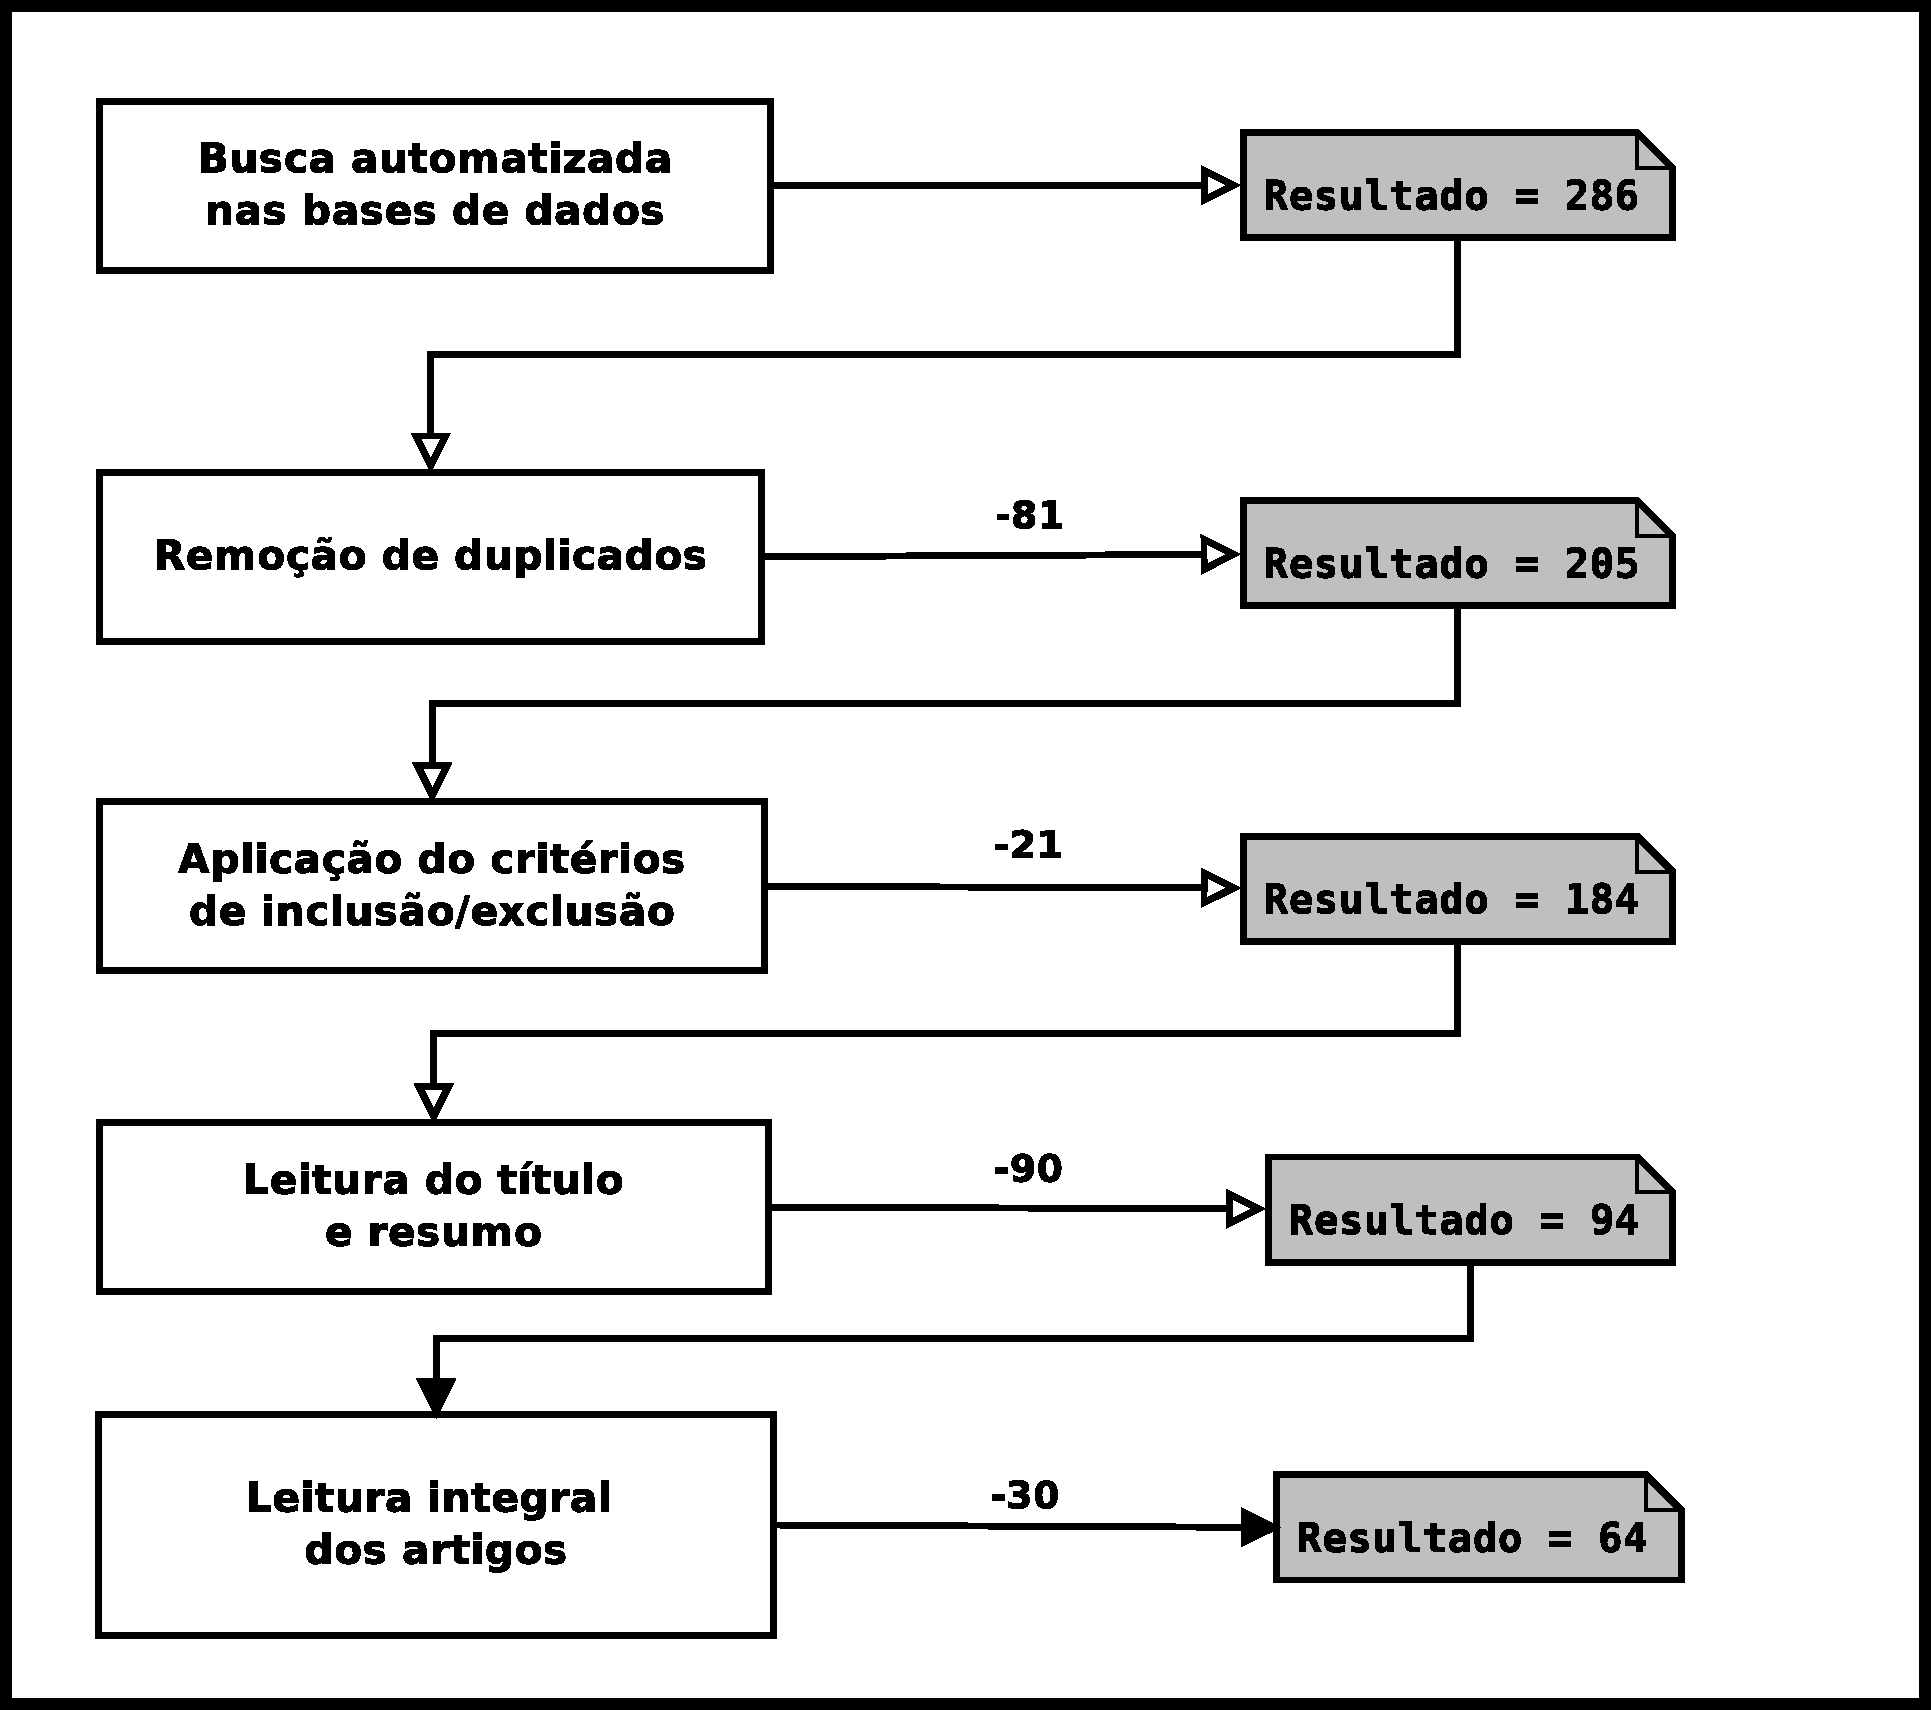
\includegraphics[width=0.75\linewidth]{./chapter-mapeamento-sistematico/img/diagrama-processo-selecao.pdf}
	\caption{Número de artigos incluídos durante o processo de seleção dos estudos. Baseado em \cite{Petersen2015}}
	\label{fig:diagrama-processo-selecao}
\end{figure}

\begin{table}[htb]
	\centering
	\caption{Número de Estudos Recuperados por Base de Dados}
	\label{tab:estudos-por-base-dados}
	\begin{tabular}{cc}
		\hline
		\textbf{Base de Dados} & \textbf{Total} \\ \hline
		ACM Digital Library    & 109            \\
		IEEE Explore           & 100            \\
		Inspec/Compendex       & 22             \\
		Scopus                 & 55             \\ \hline
	\end{tabular}

\end{table}

\subsection{Esquemas de Classificação}
\label{subsec:map-esquemas-classificacao}

Com o objetivo de mapear os estudos sobre extensões das FGRM's foram propostos quatro esquemas de classificação. O primeiro esquema organiza os artigos pelo tipo de problema da atividade de manutenção de software a extensão se propõe solucionar. A segunda categorização distribuí os estudos pelo papel no processo de manutenção de software a extensão visa dar suporte. A terceira é uma classificação baseada na taxonomia para modelos de Recuperação da Informação (Information Retrieve - IR) proposta por Cerulo e Canfora \cite{cerulo2004taxonomy}. Em particular, utilizamos este esquema tendo em vista que grande parte das extensões propostas na literatura utilizam algum tipo de suporte de modelos de IR. O último esquema apresenta quais das ferramentas existentes na indústria estão sendo estendidas na literatura. Esta taxonomia nos fornece uma visão se as extensões propostas são com um foco propositivo, ou seja, sem que exista uma implementação concreta da extensão, ou se há algum tipo de ferramenta no qual existe um maior número de extensões propostas. Em seguida discutiremos cada esquema de classificação em detalhe.

\subsubsection{Classificação por Tipo de Problema}
\label{subsubsec:map-esquema-suporte-problema}

Existem diversos problemas relacionados ao processo de Manutenção de Software. Já na década de
1980 pesquisas questionavam os profissionais envolvidos com manutenção de software quais os principais
problemas da área\cite{Lientz:1981:PAS:358790.358796}. Naturalmente a percepção dos desafios
envolvidos com a manutenção de software se altera com tempo, desta forma, é sempre válido
revisar a literatura com o objetivo de entender quais os tipos de problemas estão sendo estudados.

Neste sentido foi proposto um esquema de classificação que relaciona os estudos pelo tipo de
problema que a extensão pretende resolver. A construção da taxonomia se deu com base no processo
definido por Petersen e outros \cite{Petersen2008}, o qual é composto de duas etapas:

\begin{enumerate}[I] 
	\item analisar as palavras-chaves e conceitos que identificam as contribuições do estudo por meio da analise do título e resumo
	\item após o término da etapa I, todas as palavras chaves são combinadas a fim de construir um conjunto de categorias para no qual os artigos devem ser classificados.
\end{enumerate} 

Os autores recomendam que nos casos em que o resumo e o
título do estudo não sejam capazes de caracterizá-lo, as seções de introdução e
conclusão também devem ser analisadas. Para as bases de dados onde era informado mais de um conjunto
de palavras-chaves para um mesmo artigo, utilizamos aquelas que foram informadas pelos autores. Mediante a aplicação do processo foi
construído o esquema de classificação apresentado na Figura
\ref{fig:diagrama-esquema-problemas-manutencao}.

\begin{figure}[htpb]
	\centering
	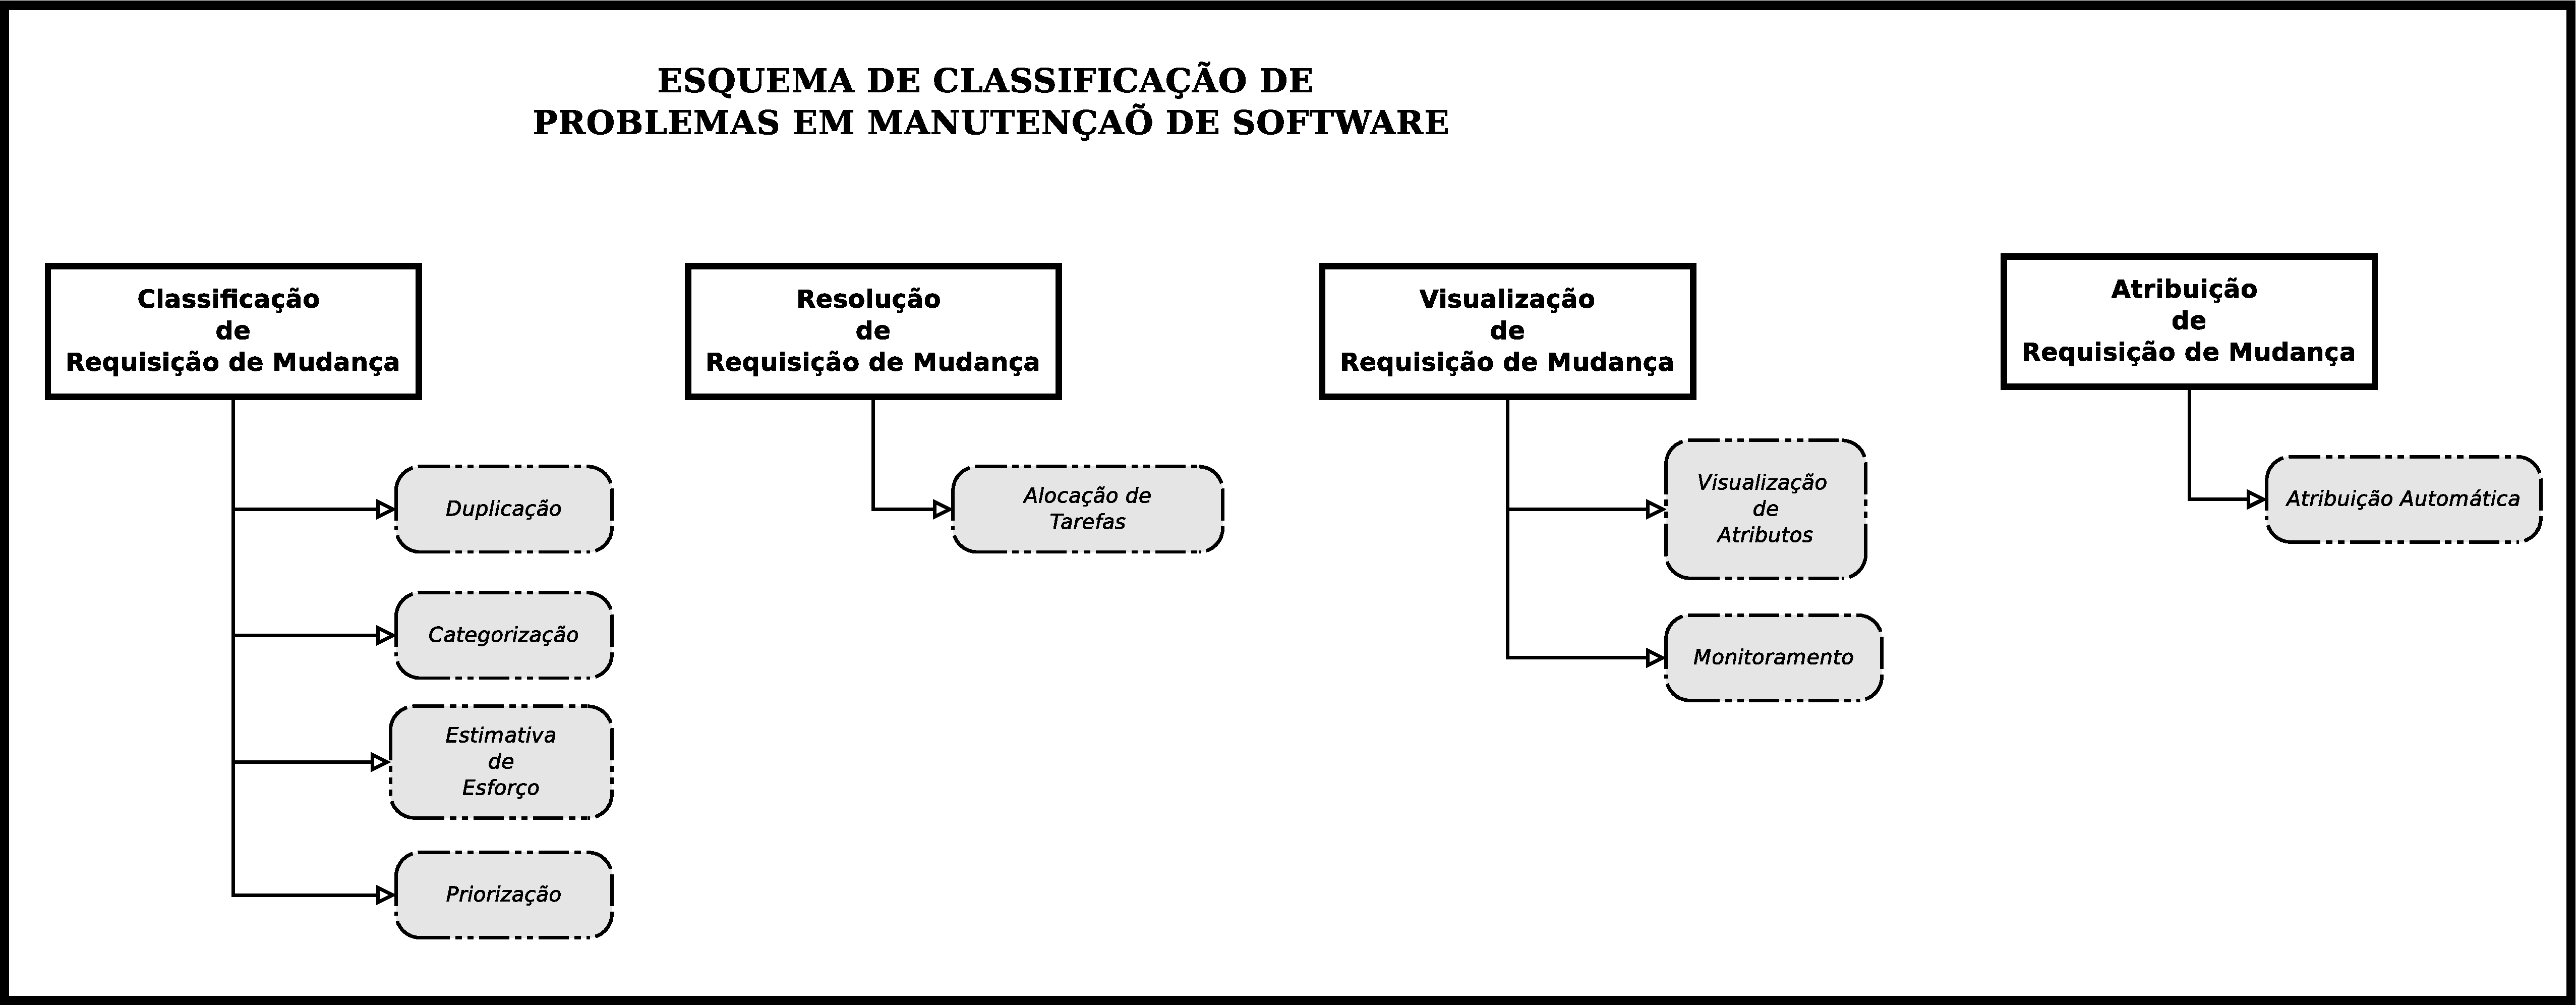
\includegraphics[width=0.8\linewidth]{./chapter-mapeamento-sistematico/img/diagrama-esquema-problemas-manutencao.pdf}
	\caption{Esquema de classificação proposto}
	\label{fig:digrama-esquema-problemas-manutencao}
\end{figure}
\todo[inline]{Incluir no anexo uma tabela demonstrando como as palavras-chaves foram combinadas}

\subsubsection{Classificação por Suporte ao Papel da Manutenção de Software}
\label{subsubsec:map-esquema-suporte-papel-man}

Da mesma forma que uma extensão proposta para as FGRM's visa resolver determinado
problema, supomos ainda que a extensão pode dar suporte a determinado papel desempenhado no processo
de Manutenção de Software. Para este fim utilizamos uma classificação modificada da proposta
por \cite{Polo1999}. No trabalho de Polo e outros o objetivo era definição de uma estrutura adequada
da equipe de manutenção de software mediante a clara identificação das tarefas que cada membro deve
executar. Os papéis propostos pelo no estudo é produto da aplicação da metodologia MANTEMA\cite{756695} para
manutenção em projetos de software bancários espanhóis, em especial aqueles em que a área de
manutenção foi terceirizada (outsourcing). Os autores reforçam que apesar da taxonomia de papéis ter
sido criada em um contexto específico, ela pode ser adequada para aplicação em outras situações.

No escopo deste trabalho a taxonomia utiliza a proposta de Polo e outros com algumas adequações. Em
especial, foram removidos os papéis que segundo o nosso entendimento estão mais vinculados a um
contexto de manutenção terceirizada (outsourcing). Além disso, dividimos o papel "time de manutenção"
(maintenance team) em \textit{Desenvolvedor e Analista de Qualidade} por entendemos que são papéis
comuns a muito dos processos de manutenção existentes. Os papéis que compõe a taxonomia proposta
estão descritos a seguir:

\begin{description}
	\item[Usuário Afetado]: Indivíduo que utiliza o sistema do qual será produzida uma Requisição de
		Mudança.
	\item[Reportador]: Responsável por registrar a Requisição de Mudança na FGRM.
	\item[Gerente de Requisição de Mudança(Maintenance-request manager)]: Responsável por decidir se
		uma Requisição de Mudança será aceita ou rejeitada e qual tipo de manutenção deverá ser
		aplicada. Posteriormente cabe a ele/ela encaminhar a RM para o Agendador.
	\item[Agendador(Scheduler)]: Deve planejar a fila de Requisições de Mudança aceitas. Também
		estão no rol de responsabilidades deste papel a atribuição das RM's para o desenvolver
		mais apto.
	\item[Desenvolvedor]: Responsável realizar as ações que irão solucionar a Requisição de Mudança.
	\item[Analista de Qualidade]: Avaliam uma Requisição de Mudança que foi solucionada por um
		Desenvolvedor afim de verificar se a RM foi corretamente resolvida.
	\item[Líder da Manutenção(Head of Maintenance)]: Tem por responsabilidade definir os padrões
		e procedimentos que compõe o processo de manutenção que será utilizado.
\end{description}

Apesar da taxonomia de papéis utilizada derivar de um contexto de manutenção de software específico
(setor bancário e empresas com a área de manutenção terceirizada), ela é capaz de acoplar com outros
tipos de processo de manutenção de software, como aquele proposto por Ihara e outros
\cite{Ihara:2009:AMI:1595808.1595833}. Naquele estudo foi criada uma representação de um processo
de modificação de bugs tomando como base as diversas situações que um bug possui em uma FGRM no contexto de projetos de código aberto. O processo resultante é facilmente acoplável com a taxonomia utilizada em
nosso estudo.

Cabe ressaltar que está fora do escopo deste estudo elaborar uma taxonomia de papeis envolvidos na
Manutenção de Software em função de supormos que isto corresponde a um esforço bem extenso. Nossa
ação é identificar quais artigos trabalham com a noção de quais papeis a extensão pretender dar
suporte,  ou seja,  relatar se existem papeis e quais são eles,  sem com isso, envolver em uma
consolidação definitiva.

\subsubsection{Classificação por Técnicas de Recuperação da Informação}
\label{subsubsec:map-esaquema-tecnicas-ir}

Um ponto em comum entre as diversas extensões para FGRM propostas na literatura é o fato delas utilizarem algum suporte de modelos de Recuperação de Informação (Information Retrieve - IR). Um modelo de IR visa solucionar um uma necessidade informacional de um usuário, representada como um conjunto de termos, no qual uma lista dos documentos mais relevantes devem ser recuperadas de uma coleção \cite{baeza1999modern}. 

Com o objetivo de obter uma visão geral das técnicas que estão sendo utilizadas para implementar as
extensões para as FGRM, realizamos a classificação dos estudos através da taxonomia proposta por
Canfora e Cerulo\cite{cerulo2004taxonomy}. O esquema de classificação consiste em duas visões
sobrepostas: uma taxonomia vertical que classifica os modelos de IR com relação ao seu conjunto
de características básicas; e uma taxonomia horizontal que classifica os objetos de IR com respeito
as suas tarefas, forma e contexto\cite{cerulo2004taxonomy}. Nesta dissertação utilizamos a
classificação vertical tendo em vista que estamos interessados na técnica utilizada na implementação da extensão.

\todo[inline]{Verificar a necessidade de definir melhor alguns termos de IR. Ex. documento, consulta
do usuário, problema da representação de similaridade}

\todo[inline]{Verificar o total de artigos que utilizam algum técnica de IR. Apesar de grande parte
utilizar não serão todos os artigos}

A taxonomia vertical é construída explorando duas características básicas de um Modelo de
Recuperação da Informação: \textit{representação (representation)}, que é a forma adotada para representar ao mesmo
tempo o documento e consulta do usuário; \textit{raciocínio (reasoning)}, ao qual se refere ao framework adotado
para resolver o problema da representação de similaridade, ou seja, trata-se do conjunto de métodos, modelos e tecnologias utilizadas para realizar o casamento entre um documento e a consulta do usuário. O esquema de classificação proposto pelos autores é apresentado na Figura \ref{fig:information-retrieval-model}.

\begin{figure}[htpb]
	\centering
	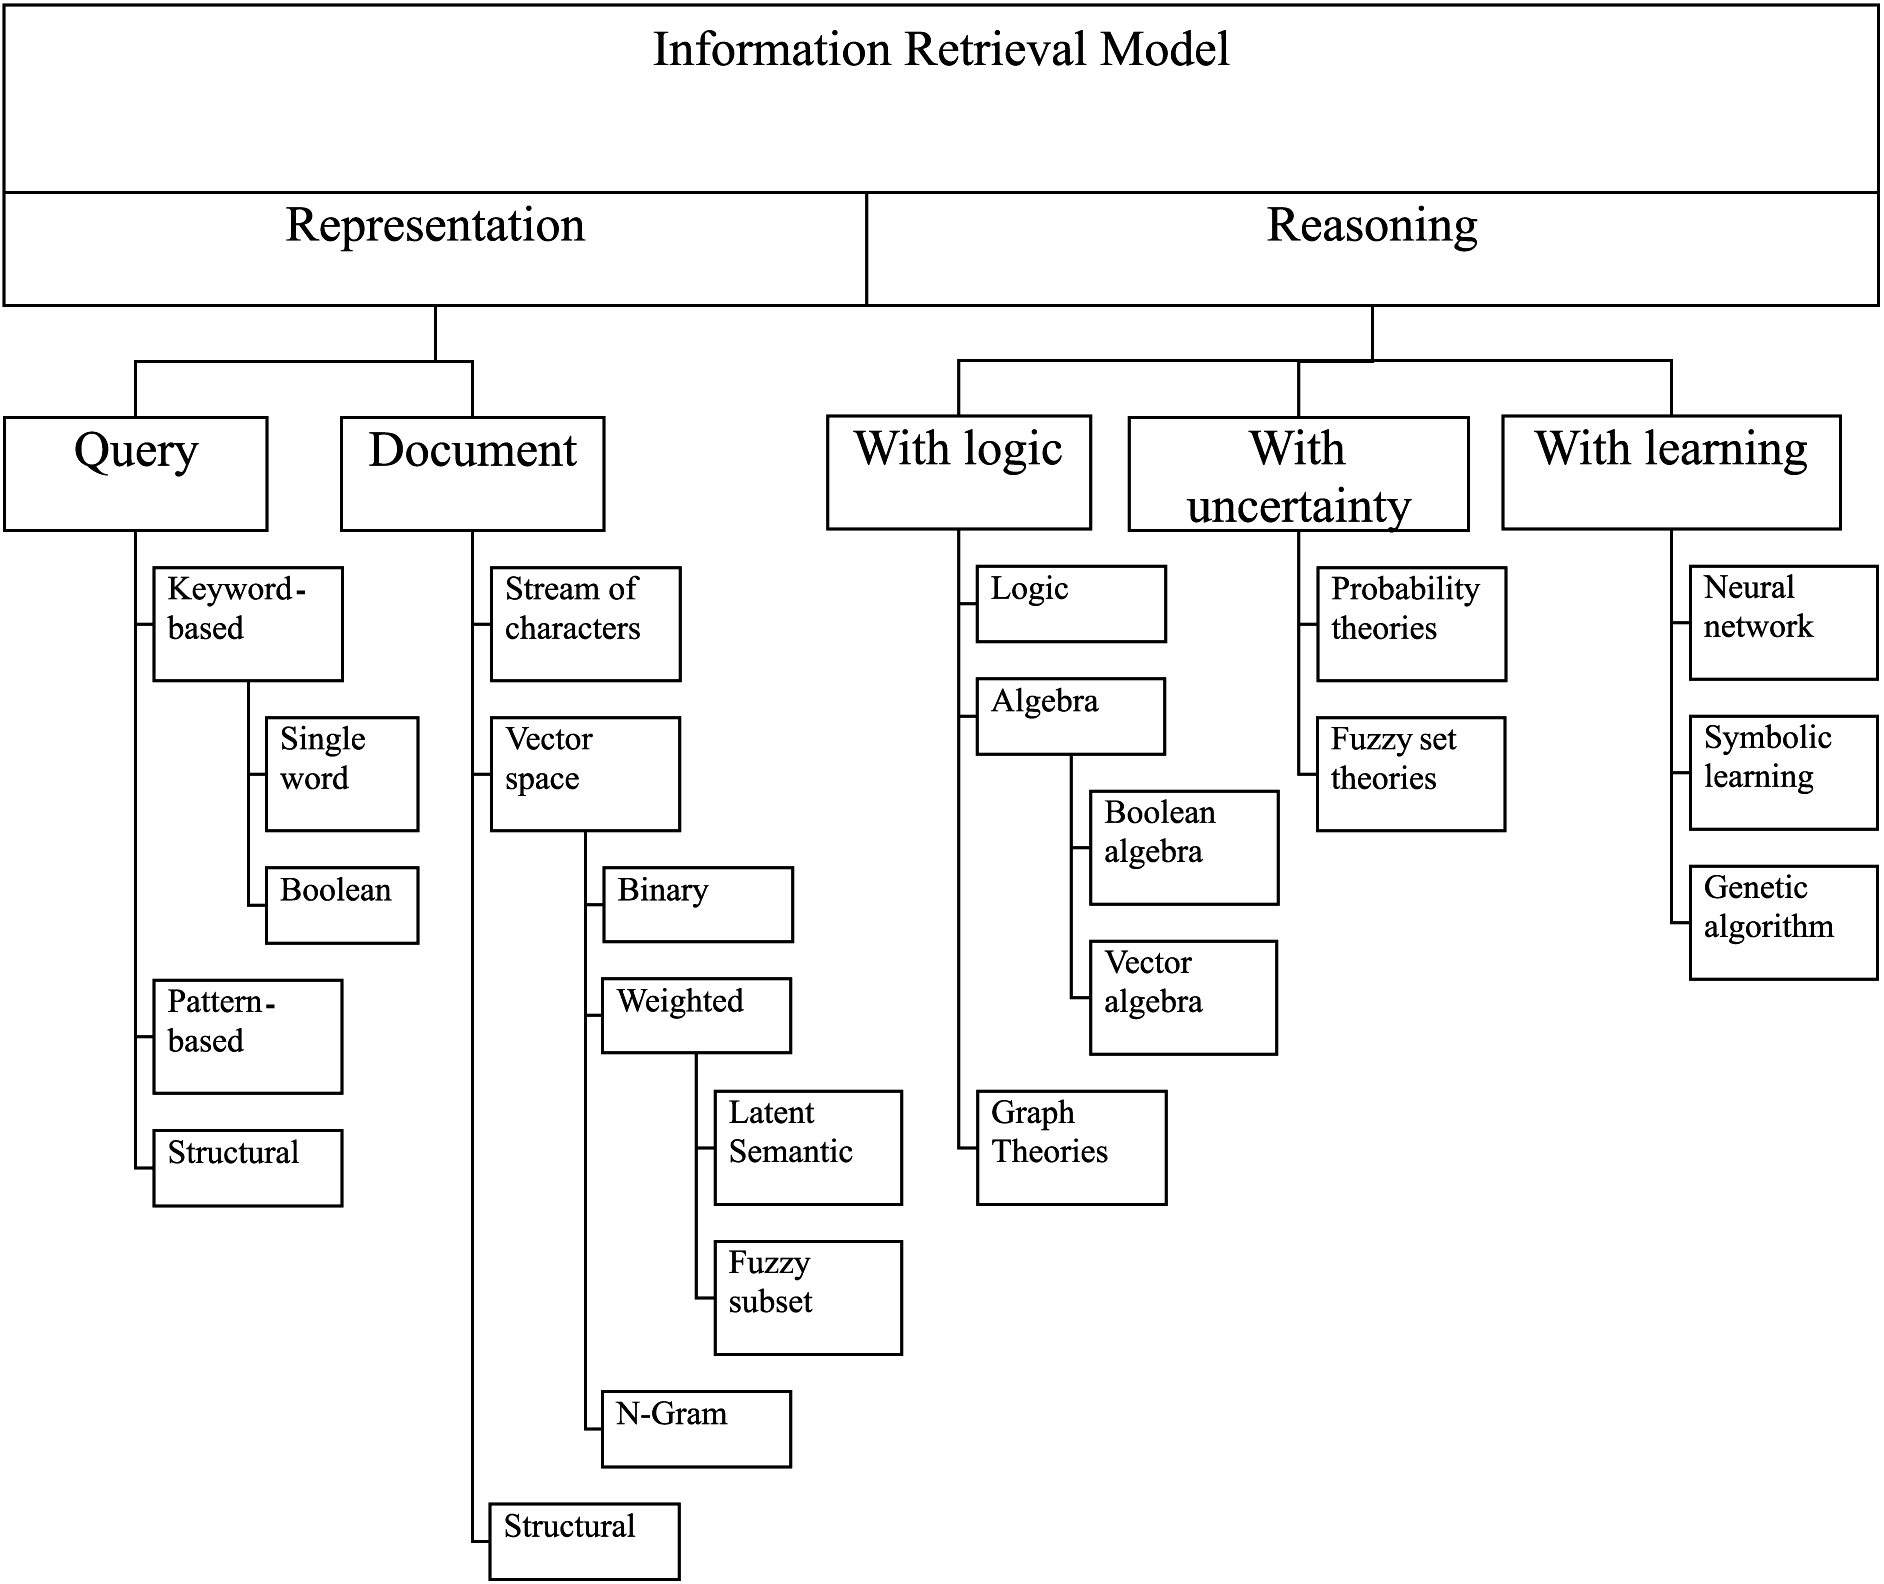
\includegraphics[width=0.8\linewidth]{./chapter-mapeamento-sistematico/img/information-retrieval-model.png}
	\caption{Taxonomia vertical para Modelos de Recuperação da Informação. Adaptado de \cite{cerulo2004taxonomy}}
	\label{fig:information-retrieval-model}
\end{figure}

\subsubsection{Classificação por Ferramenta Estendida}
\label{subsubsec:map-esquema-ferramenta}

Do ponto de vista dos profissionais envolvidos em Manutenção de Software é importante entender quais as FGRM estão sendo estendidas. Por outro lado, para os pesquisadores é importante descobrir aquelas ferramentas mais "amigáveis" para o desenvolvimento de novas extensões bem como a melhoria das existentes. Neste sentido, realizamos a classificação dos estudos pelas ferramentas que foram utilizados para o desenvolvimento das extensões. Uma ferramenta é entendida como utilizada por determinado estudo se ela foi utilizada no processo de validação ou se seus dados foram utilizados na avaliação da extensão. 

Para produzirmos a taxonomia realizarmos a leitura do resumo e da introdução do artigo. Nos casos em que não foi possível determinar a ferramenta utilizada a partir da leitura das seções citadas, procedemos com a leitura com a parte avaliação do estudo. A Tabela exibe as ferramentas utilizadas para cada estudo analisado.


\section{Resultados}
\label{sec:resutaldos}

Nesta seção apresentamos os resultados do Mapeamento Sistemático. Cada uma das taxonomias propostas
é analisada mediante a apresentação dos estudos que possam exemplificar a classificação adotada.
Iniciamos pela classificação por problemas na Manutenção de Software, o qual dividimos os estudos
por área e tópico de pesquisa. Seguimos com a análise dos estudo pelo papel ao qual a extensão visa
dar suporte. Posteriormente analisamos os modelos de IR utilizados para implementar algumas das
extensões propostas na literatura. Finalizamos esta análise com as ferramentas existentes no mercado
que estão efetivamente sendo entendidas.

\subsection{Extensões para Problemas na Manutenção de Software}
\label{sub:extensões_para_problemas_na_manutenção_de_software}

Nesta etapa do trabalho estamos interessados no estado da arte do estudo dos problemas encontrados
na Manutenção de Software. Em especial, o nosso foco é entender que tipo de extensão para FGRM estão
sendo proposta para solucionar este tipo de problema. Com base no mapeamento sistemático realizado a
classificação do estudos é apresentada na Tabela \ref{tab:taxonomia-problemas-manutencao}.


O total de artigos por área de pesquisa e seus respectivos tópicos pode ser observado na Figura
\ref{fig:bubble-plo-problema-manutencao}

% Inclusão da tabela
\begin{table}[htbp]
\centering
\caption{My caption}
\label{my-label}
\resizebox{\textwidth}{!}{%
\begin{tabular}{|c|l|l|c|}
\hline
\textbf{Dimensão da Melhoria} & \multicolumn{1}{c|}{\textbf{Tópico}}             & \multicolumn{1}{c|}{\textbf{Estudos}}          & \textbf{Total}       \\ \hline
\multirow{13}{*}{Ferramenta}  & Busca de RM                                      & \cite{Liu2014}                                 & 1                    \\ \cline{2-4} 
                              & \multirow{7}{*}{Localização do Problema}         & \cite{Bangcharoensap:2012:LSC:2419061.2419428} & \multirow{7}{*}{7}   \\
                              &                                                  & \cite{Corley2011}                              &                      \\
                              &                                                  & \cite{Nguyen:2012:MAR:2393596.2393671}         &                      \\
                              &                                                  & \cite{Romo:2015:TAT:2745802.2745833}           &                      \\
                              &                                                  & \cite{thung2013automatic}                      &                      \\
                              &                                                  & \cite{Thung:2014:BIT:2635868.2661678}          &                      \\
                              &                                                  & \cite{Wong:2014:BBF:2705615.2706096}           &                      \\ \cline{2-4} 
                              & Monitoramento de RM                              & \cite{Aggarwal:2014:MIT:2593801.2593810}       & 1                    \\ \cline{2-4} 
                              & \multirow{4}{*}{Visualização de RM}              & \cite{dal2013closer}                           & \multirow{4}{*}{4}   \\
                              &                                                  & \cite{Hora2012}                                &                      \\
                              &                                                  & \cite{Sasso2014}                               &                      \\
                              &                                                  & \cite{takama2013application}                   &                      \\ \hline
\multirow{9}{*}{Informação}   & \multirow{2}{*}{Organização da Informação da RM} & \cite{mani2012ausum}                           & \multirow{2}{*}{2}   \\
                              &                                                  & \cite{Otoom2016}                               &                      \\ \cline{2-4} 
                              & \multirow{7}{*}{Suporte ao Registro da RM}       & \cite{Bettenburg2008a}                         & \multirow{7}{*}{7}   \\
                              &                                                  & \cite{Correa2013b}                             &                      \\
                              &                                                  & \cite{moran2015auto}                           &                      \\
                              &                                                  & \cite{Moran:2015:EAA:2786805.2807557}          &                      \\
                              &                                                  & \cite{Tu:2014:MQI:2677832.2677844}             &                      \\
                              &                                                  & \cite{White:2015:GRR:2820282.2820291}          &                      \\
                              &                                                  & \cite{Wu2011a}                                 &                      \\ \hline
\multirow{40}{*}{Processo}    & \multirow{12}{*}{Atribuição (Triagem) de RM}     & \cite{Banitaan2013}                            & \multirow{12}{*}{12} \\
                              &                                                  & \cite{hosseini2012market}                      &                      \\
                              &                                                  & \cite{Hu:2014:EBT:2707683.2708297}             &                      \\
                              &                                                  & \cite{Naguib2013}                              &                      \\
                              &                                                  & \cite{Nagwani2012}                             &                      \\
                              &                                                  & \cite{shokripour2012automatic}                 &                      \\
                              &                                                  & \cite{tian2015automated}                       &                      \\
                              &                                                  & \cite{ValdiviaGarcia:2014:CPB:2597073.2597099} &                      \\
                              &                                                  & \cite{Wu2011}                                  &                      \\
                              &                                                  & \cite{Xuan:2012:DPB:2337223.2337227}           &                      \\
                              &                                                  & \cite{Zanetti2013}                             &                      \\
                              &                                                  & \cite{Zhang2014}                               &                      \\ \cline{2-4} 
                              & \multirow{10}{*}{Classificação de RM}            & \cite{behl2014bug}                             & \multirow{10}{*}{10} \\
                              &                                                  & \cite{chawla2015automated}                     &                      \\
                              &                                                  & \cite{Gegick2010}                              &                      \\
                              &                                                  & \cite{Izquierdo2015}                           &                      \\
                              &                                                  & \cite{kochhar2014automatic}                    &                      \\
                              &                                                  & \cite{Nagwani2013}                             &                      \\
                              &                                                  & \cite{netto2010automated}                      &                      \\
                              &                                                  & \cite{somasundaram2012automatic}               &                      \\
                              &                                                  & \cite{Tian:2013:DPP:2550526.2550574}           &                      \\
                              &                                                  & \cite{zhang2011bug}                            &                      \\ \cline{2-4} 
                              & \multirow{5}{*}{Estima de Esforço da RM}         & \cite{Bhattacharya:2011:BTP:1985441.1985472}   & \multirow{5}{*}{5}   \\
                              &                                                  & \cite{Nagwani2010}                             &                      \\
                              &                                                  & \cite{Thung2012}                               &                      \\
                              &                                                  & \cite{Vijayakumar2014}                         &                      \\
                              &                                                  & \cite{xia2015automatic}                        &                      \\ \cline{2-4} 
                              & \multirow{13}{*}{Localização de RM Duplicados}   & \cite{alipour2013contextual}                   & \multirow{13}{*}{13} \\
                              &                                                  & \cite{banerjee2012automated}                   &                      \\
                              &                                                  & \cite{hindle2016contextual}                    &                      \\
                              &                                                  & \cite{Koopaei:2015:CAD:2886444.2886474}        &                      \\
                              &                                                  & \cite{Lerch:2013:FDY:2495256.2495763}          &                      \\
                              &                                                  & \cite{Liu:2012:TBR:2393596.2393628}            &                      \\
                              &                                                  & \cite{Prifti2011}                              &                      \\
                              &                                                  & \cite{Song2010a}                               &                      \\
                              &                                                  & \cite{sun2010discriminative}                   &                      \\
                              &                                                  & \cite{Sun2011}                                 &                      \\
                              &                                                  & \cite{Thung2014}                               &                      \\
                              &                                                  & \cite{Tian2012}                                &                      \\
                              &                                                  & \cite{Tomasev2013}                             &                      \\ \hline
\multirow{2}{*}{Usuário}      & \multirow{2}{*}{Recomendação de RM}              & \cite{malheiros2012source}                     & \multirow{2}{*}{2}   \\
                              &                                                  & \cite{Wang2011a}                               &                      \\ \hline
\end{tabular}%
}
\end{table}


\begin{figure}[htpb]
	\centering
	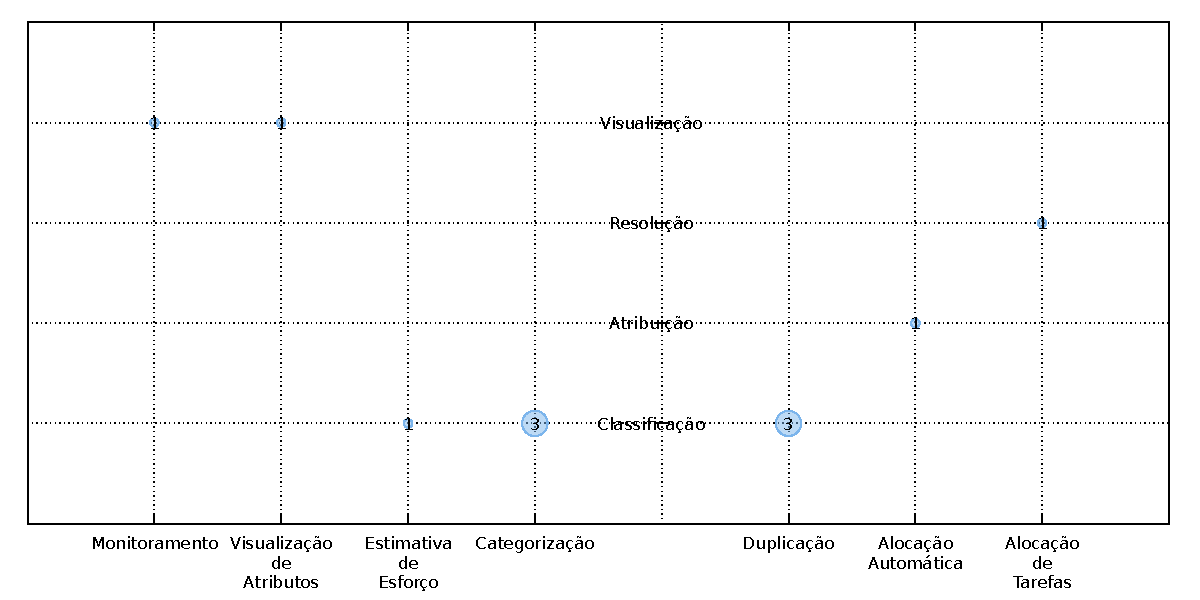
\includegraphics[width=0.8\linewidth]{./chapter-mapeamento-sistematico/img/bubble-plot-problema-manutencao.pdf}
	\caption{Total de artigos por categoria de problema}
	\label{fig:bubble-plot-problema-manutencao}
\end{figure}
\subsubsection{Classificação de Requisições de Mudança}
\label{ssub:classificação_de_requisições_de_mudança}

\subsubsection{Duplicação}
\subsubsection{Categorização}
\subsubsection{Estimativa de Esforço}



\subsection{Extensões com Suporte à Papeis}
\label{sub:extensões_com_suporte_à_papeis}


\subsection{Técnicas de IR Utilizadas pelas Extensões}
\label{sub:técnicas_de_ir_utilizadaas_pelas_extensões}


\subsection{Ferramentais Estendidas}
\label{sub:ferrramentas_extendidas}


\section{Limitações e Ameaças à Validade}

\section{Trabalhos Relacionados}

\section{Resumo do Capítulo}

%Incluindo o fonte do Capítulo 04
%%%%%%%%%%%%%%%%%%%%%%%%%%%%%%%%%%%%%%%%%%%%%%%%%%%%%%%%%%%%%%%%%%%%%%%%%%%%%%%%%%%%%%%%%%%%%%%%%%%%%%%%%%%%
%Objetivo:
%Autor:
%Data Criação:
%Data Modificação:
%Data Revisão:
%%%%%%%%%%%%%%%%%%%%%%%%%%%%%%%%%%%%%%%%%%%%%%%%%%%%%%%%%%%%%%%%%%%%%%%%%%%%%%%%%%%%%%%%%%%%%%%%%%%%%%%%%%%%
\chapter{Caracterização das Ferramentas de Gerenciamento de Requisição de Mudança}
\label{ch:caracterizacao}


\section{Introdução}
\todo[inline]{Definir conforme livro do wohlin(é assim que escreve??) o conceito de estudo
	exploratório}
Esta etapa do trabalho consiste de um estudo exploratório com o objetivo de determinar quais são as funcionalidades comuns às Ferramentas de Gerenciamento de Requisição de Mudança (FGRM). O estudo consistirá na leitura da documentação de alguns FGRM para que de forma sistemática seja levantado quais são as funcionalidades oferecidas pela ferramenta em análise. O método de escolha das FGRM será avaliado posteriormente, todavia, um possível ponto de partida é a lista disponível na Wikipédia que compara diversas FGRM\footnote{\url{https://en.wikipedia.org/wiki/Comparison_of_issue-tracking_systems}}.

\section{Objetivo do Capítulo}
\label{sec:objetivo_do_capítulo}

Neste capítulo realizamos um estudo exploratório com o objetivo de determinar as
funcionalidades comuns as Ferramentas de Gerenciamento de Requisição de Mudanças existentes no
mercado. A partir deste conjunto de compartilhado de funcionalidades é possível avaliar a
contribuição das extensões que estão sendo propostas na literatura, conforme discutido no
Capítulo\ref{ch:mapeamento-sistematico}.

Acreditamos que o resultado deste estudo permitirá compreender melhor este tipo de ferramenta tomando como base as
suas funcionalidades em comum. Também será possível propor extensões para as FGRM tendo em vista a
possibilidade de determinar o conjunto mínimo de funções deste tipo de sistema. Uma outra possível
contribuição é a possibilidade de criação de um esquema de caracterização com base nas funcionalidades oferecidas.

\section{Metodologia}
\label{sec:metodologia}

O processo de descoberta das funcionalidades comuns às FGRM é composto das etapas descritas a
seguir:

\begin{itemize}
	\item Seleção das Ferramentas
	\item Inspeção da Documentação
	\item Agrupamento das Funcionalidades
\end{itemize}

Cada uma etapas é explicada em detalhes nas próximas seções. 

\subsection{Seleção das Ferramentas}
\label{ssub:Seleção das Ferramentas}

A primeira etapa consistiu na definição das ferramentas que seriam utilizadas neste estudo. Em uma
inspeção inicial, verificamos a existência de mais de 50 FGRM disponíveis comercialmente ou de
código aberto\footnote{\url{https://en.wikipedia.org/wiki/Comparison_of_issue-tracking_systems}}. Contudo,
devido a dificuldade de realizar a análise de cada uma daquelas ferramentas, optamos por escolher um
subconjunto das ferramentas que fosse mais representativas, segundo o nosso conhecimento na área. A
representatividade neste caso corresponde a notoriedade que a ferramenta possui dentro da literatura
(Ex. Bugzilla) ou mesmo na industria (Ex. Github).
\todo[inline]{Conforme sugestão do professor Rodolfo seria interessante avaliar quais das ferramentas
têm real notoriedade com base na opinião de profissionais envolvidos em manutenção de software}

As FGRM selecionadas foram inicialmente classificadas como \textit{"ferramentas"} e
\textit{"serviços da internet"}. O primeiro grupo representa os softwares capazes de serem implantados
na infraestrutura do seu cliente e do qual permite algum grau de personalização de alguns
componentes, como por exemplo o bando de dados utilizado. No segundo grupo estão os software que
ofertam a gerência das RM's mediante uma arquitetura do tipo Software como Serviço (Software as
Service), onde certos tipos de alterações no comportamento do software por parte do usuário são mais restritas. As
ferramentas selecionadas são apresentadas por tipo de categoria na Tabela
\ref{tab:ferramentas_selecionadas}
\todo[inline]{Incluir referência sobre Software como Serviço}

\begin{table}[ht]
	\centering
	\caption{Ferramentas e serviços da Internet selecionados.}
	\resizebox{\textwidth}{!}{%
		\begin{tabular}{llll}
			\hline
			\multicolumn{2}{c}{\textbf{Ferramentas}}           & \multicolumn{2}{c}{\textbf{Serviços da Internet}} \\ \hline
			Bugzilla & \url{https://www.bugzilla.org/}              & SourceForge    &
			\url{https://sourceforge.net/}    \\ \hline
			MantisBT & \url{https://www.mantisbt.org/}               & Lauchpad       &
			\url{https://launchpad.net/}      \\ \hline
			Trac     & \url{https://trac.edgewall.org/}              & Code Plex      &
			\url{https://www.codeplex.com/}   \\ \hline
			Redmine  & \url{www.redmine.org/}                        & GitLab			&
				\url{https://gitlab.com}          \\ \hline
			Jira     & \url{https://www.atlassian.com/software/jira} & GitHub         &
				\url{https://github.com/}         \\ \hline
		\end{tabular}%
	}
	\label{tab:ferramentas_selecionadas}
\end{table}

\subsection{Inspeção da Documentação}
\label{ssub:Inspeção da Documentação}

Neste etapa do trabalho realizamos a leitura do material disponível na internet para cada uma das
ferramentas. Entre estes materiais inclui manual do usuário, manual do desenvolvedor, notas de
lançamento e etc. Para cada uma das FGRM optamos por analisar a última versão estável do software a
fim de analisarmos o que há de mais novo disponível aos usuários. A Tabela apresenta a versão
analisada e o elo de ligação para cada uma da documentação utilizada neste estudo. Para aquelas
ferramentas que apresentam documentação em mais de um idioma optamos sempre por utilizar aquela
escrita em inglês por entendermos ser a que possivelmente mais atualizada.

\subsection{Agrupamento das Funcionalidades}
\label{ssub:Agrupamento das Funcionalidades}

Esta etapa tem por objetivo agrupar as funcionalidades que aparecem com nomenclatura distintas em
diferentes ferramentas, mas que apresentam o mesmo significado. Cabe ressaltar que o agrupamento de
algumas funcionalidades pode depender de uma análise subjetiva de quem está realizando a atividade.
Neste sentido, a fim de evitar algum tipo de viés o agrupamento foi realizado em duas etapas:

\begin{description}
	\item[Análise Individual] Neste etapa o autor e um outro especialista realizam de forma separada
		os agrupamentos que acharem necessários
	\item[Anaĺise Compartilhada] Em um segundo momento tanto o auto quanto o especialista discutem
		as possíveis divergências até que um consenso seja obtido.	
\end{description}

Após as duas etapas descritas anteriormente chegamos ao conjunto de funcionalidades descritos na
Tabela. A coluna agrupamento exibe o nome comum para representas as funções descritas na coluna
"nomenclatura original"


\section{Resultados}
\label{sec:resultados}



\section{Discussão}
\label{sec:discussao}

\section{Ameças à Validade}
\label{sec:ameacas_a_validade}


\section{Resumo do Capítulo}
\label{sec:resumo_do_capitulo}

%Incluindo o fonte do Capítulo 05
%%%%%%%%%%%%%%%%%%%%%%%%%%%%%%%%%%%%%%%%%%%%%%%%%%%%%%%%%%%%%%%%%%%%%%%%%
%Objetivo: Realizar uma pesquisa com profissionais envolvidos em manutenção de
%		   software a fim de verificar a situação atual das funcionalidades
%		   oferecias pelas FGRM.
%Autor: Vagner Clementino<vagnercs@dcc.ufmg.br> e
%		Rodolfo Resende<rodolfo@dcc.ufmg.br>
%Data Criação: sex fev  3 19:57:56 BRST 2017
%Data Modificação: qui abr  6 20:33:42 -03 2017
%Data Revisão: qui abr  6 21:01:54 -03 2017
%%%%%%%%%%%%%%%%%%%%%%%%%%%%%%%%%%%%%%%%%%%%%%%%%%%%%%%%%%%%%%%%%%%%%%%%%%
\chapter{Levantamento por Questionário com Profissionais}
\label{ch:pesquisa-profissionais}

\section{Introdução}
\label{sec:pesquisa-profissionais-intro}

Um levantamento por questionários, conhecido na literatura como
\textit{Survey}, é uma abordagem de coleta e análise de dados em que os
participantes respondem a perguntas ou declarações que foram desenvolvidas
Este tipo de estudo permite que os pesquisadores generalizem as crenças e
opiniões de uma população mediante os dados coletados de um subconjunto do
público-alvo (amostra). No trabalho conduzido por
Kasunic~\cite{kasunic2005designing} são apresentadas uma sequência de etapas a
serem seguidas no processo de condução deste tipo de trabalho:

\begin{enumerate}
\item{Identificar os objetivos da pesquisa}
\item{Identificar e caracterizar o público-alvo}
\item{Elaborar o plano de amostragem}
\item{Elaborar e escrever um questionário}
\item{Aplicar questionário de teste ou piloto}
\item{Distribuir o questionário}
\item{Analisar os resultados e escrever o relatório}
\end{enumerate}

Com o objetivo de coletar os aspectos mais importantes das funcionalidades
oferecidas pelas Ferramentas de Gerenciamento de Requisições de Mudança (FGRMs),
do ponto de vista dos profissionais ligados à manutenção de software, realizamos
um levantamento mediante questionário. O planejamento e o desenho do estudo
seguiu as diretrizes propostas nos trabalhos de
Wohlin~\cite{wohlin2012experimentation} e Kasunic~\cite{kasunic2005designing}.
Em especial, no tocante a definição da população e da amostra de interesse
utilizamos o arcabouço (framework) proposto por De Mello e
outros~\cite{de2015investigating, de2014towards}.

A população da pesquisa é a comunidade envolvida com o processo de manutenção de
software e que faça uso de FGRMs. Neste sentido, utilizamos como amostra os
profissionais que estão envolvidos no projeto de código aberto
Python\footnote{\url{http://bugs.python.org/}}. Por outro lado, visando alcançar
profissionais que trabalham em empresas privadas, utilizamos os usuários da
rede social de desenvolvedores Stack
Overflow\footnote{\url{http://stackoverflow.com}}. Neste último caso, estamos
interessados nos usuários da rede que tenham participado de discussões sobre
assuntos relacionados à manutenção de software. A pesquisa foi replicada em uma
empresa pública de software do qual o autor possui vínculo. Maiores detalhes
sobre o processo de escolha das amostras serão discutidos posteriormente.

A importância deste tipo de trabalho está na possibilidade de avaliar se as
pesquisas relativas a evolução das funcionalidades das FGRMs estão em
consonância com as necessidades dos profissionais. Neste sentido é possível
discutir a distância entre o estado da arte e o estado da prática.

\section{Objetivo do Levantamento com Profissionais}
\label{sec:objetivo_da_pesquisa_com_profissionais}

Em linhas gerais, o objetivo desta etapa da dissertação é analisar, através da
percepção e opinião dos profissionais envolvidos em manutenção de software, a
situação das funcionalidades atualmente oferecidas pelas FGRMs, bem como a
adotação das metodologias propostos pelos agilistas no processo de manutenção de
software. Colocando a finalidade do levantamento conforme propõe a metodologia
GQM (Goal, Question e Metric)\cite{gqm}, \textit{o propósito deste estudo é
	avaliar as funcionalidades oferecidas pelas FGRMs e as melhorias propostas
	nas literatura, do ponto de vista dos
	profissionais envolvidos em manutenção de software no contexto de projetos
	de software de código aberto e uma empresas publicas e privadas de
	informática.}

Com intuito de atingir os objetivos propostos foram definidas as seguintes
questões de pesquisa:

\begin{description}
	\item[Questão 01] Qual a opinião dos profissionais envolvidos em Manutenção
		de Software com relação as funcionalidades oferecidas atualmente pelas
		FGRM\@?
	\item[Questão 02] Na visão dos profissionais envolvidos em Manutenção de
		Software quais das extensões propostas na literatura teriam maior
		relevância em suas atividades atuais?
	\item[Questão 03] Como as práticas propostas pelos agilistas estão sendo
	utilizadas especialmente no processo de manutenção de software?
	\item[Questão 04] Como as FGRMs podem ajudar aos times devotados à manutenção
	de software na prática adotada pelos agilistas?
\end{description}

O desenho da pesquisa é detalhado na próxima seção onde discutimos a estrutura
do questionário bem como a amostra da população que foi utilizada.

\section{Desenho e Metodologia da Pesquisa com Profissionais}
\label{sec:desenho_da_pesquisa_com_profissionais}

\subsection{Conceitos Básicos}

Estudos primários em Engenharia de Software (SE), como os levantamentos por
questionários, são muitas vezes conduzidos em amostras estabelecidas por
conveniência~\cite{sjoberg2005survey, dybaa2006systematic}. Um desafio no
estabelecimento de amostras representativas nos levantamentos, especialmente em
Engenharia de Software, é a identificação de fontes relevantes e disponíveis que
permitam criar as amostragem~\cite{de2014towards}. Uma alternativa é a
utilização de fontes disponíveis na Internet, como as rede sociais, para
aumentar o tamanho da amostra~\cite{de2013would}. Outra fonte que pode aumentar
a significância das amostras são os projetos de código e seus respectivos
artefatos.

O nosso levantamento com profissionais consistiu de um estudo exploratório sem
uma hipótese prévia. Conforme discutido anteriormente, a população de interesse
desta pesquisa é composta por profissionais envolvidos em desenvolvimento e
manutenção de software. Para sistematizar o processo de escolha da amostragem
utilizamos o arcabouço (framework) conceitual proposto por de Mello e
outros~\cite{de2014towards} que está representado na
Figura~\ref{fig:framework-amostragem}. O modelo proposto inclui além dos
conceitos estatísticos tradicionalmente utilizados em levantamentos com
questionário, tais como público-alvo, população, amostragem e unidade de
observação~\cite{thompson2012sampling}, introduz um conjunto de novos conceitos
que visam apoiar o processo de escolha da amostragem. Os conceitos que os
autores propuserem incluem: \textit{Fonte de Amostragem, Unidade de Pesquisa,
	Plano de Pesquisa e Estratégia de Amostragem}.

\begin{figure}[htpb]
	\centering
	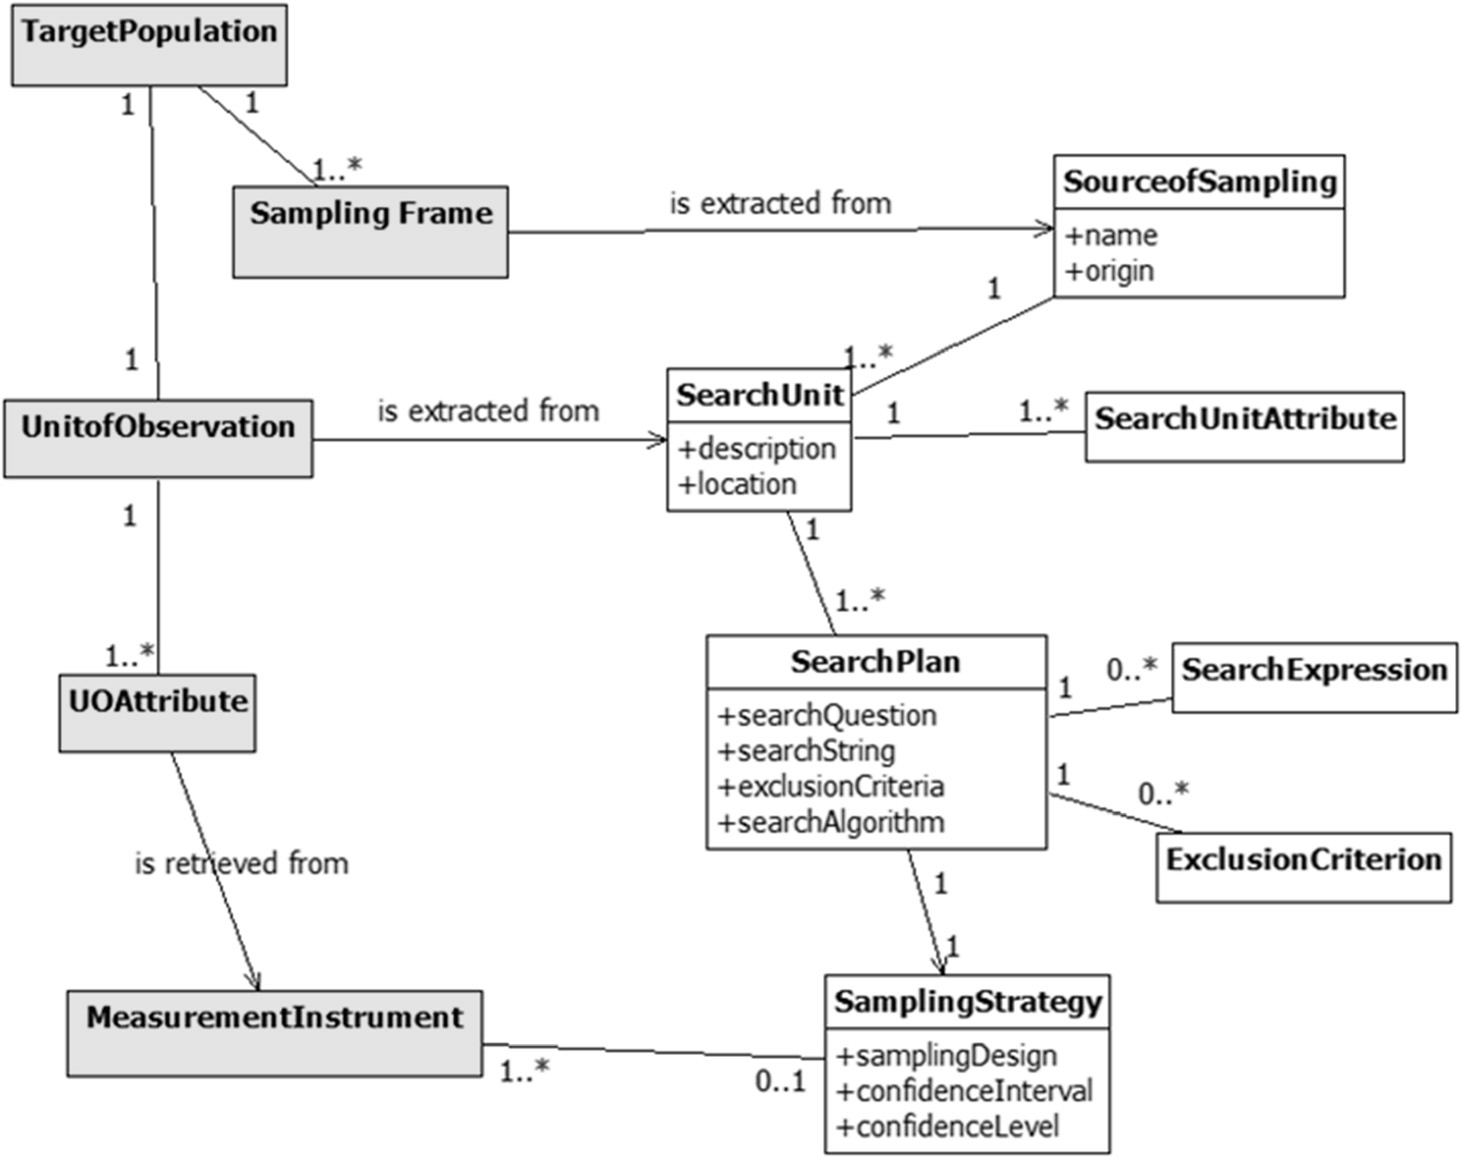
\includegraphics[width=0.6\linewidth]{./chapter-pesquisa-com-profissionais/img/framework-amostragem.png}
	\caption{Os conceitos que compõem o Arcabouço Conceitual proposto por de
		Mello. Extraído de~\cite{de2015investigating}}
\label{fig:framework-amostragem}
\end{figure}

A \textit{Unidade de Observação} é a entidade que é estudada em determinado
experimento~\cite{wohlin2012experimentation}. Uma Unidade pode ser produtos,
processos, recursos, modelos, métricas, teorias ou pessoas. Uma \textit{Unidade
	de Pesquisa} caracteriza como uma ou mais \textit{Unidade de Observação}
podem ser recuperadas de uma \textit{Fonte de Amostragem} específica. O
\textit{Plano de Pesquisa} descreve como \textit{Unidades de Pesquisa} serão
sistematicamente recuperadas de uma Fonte de Amostragem e avaliadas para compor
a amostragem da pesquisa. Finalmente, a Estratégia de Amostragem descreve as
etapas que devem ser seguidas para definição da amostragem e recrutamento de
indivíduos que participarão do estudo.

Uma \textit{Fonte de Amostragem} consiste de um banco de dados, que não
necessariamente é automatizado, em que um subconjunto válido do público-alvo
pode ser sistematicamente recuperado, além de permitir a extração aleatória de
amostras da população de interesse. Sendo assim, os autores~\cite{de2014towards}
afirmam que no caso de determinada Fonte de Amostragem ser considerada válida
para um contexto de pesquisa específico, pode-se concluir que as amostras podem
ser extraídas desta fonte a fim de serem utilizados no mesmo contexto de
pesquisa. Para ser considerada válida, uma Fonte de Amostragem deve satisfazer,
pelo menos, aos seguintes Requisitos Essenciais (Essential Requirements\@-\@ ER):

\begin{description}
	\item[ER1] Uma Fonte de Amostragem não deve representar intencionalmente um
		subconjunto segregado do público-alvo, ou seja, dado um público-alvo
		\textit{``X''}, não seria adequado pesquisar por unidades na Fonte
		intencionalmente desenhada para compor um subconjunto específico de
		\textit{``X''}.
	\item[ER2] Uma Fonte de Amostragem não deve apresentar qualquer viés em
		incluir na sua base de dados determinados subconjuntos do público-alvo.
		Critérios desiguais para inclusão de Unidades de Pesquisa significam
		oportunidades desiguais para oportunidades de amostragem.
	\item[ER3] Todas as Unidades de Pesquisa das amostras e suas Unidades de
		Observação devem identificados por de forma única.
	\item[ER4] Todas as amostragem de determinada Unidade de Pesquisa devem ser
		acessíveis. Se houver unidades de pesquisa ocultas, não é possível
		contextualizar a população.
\end{description}

O estudo realizado por de Mello~\cite{de2014towards} cita outros requisitos que
são definidos como desejáveis que estão relacionados com amostragem, clareza e
integridade da amostra. Contudo, neste trabalho, a Fonte de Amostragem foi
valiada apenas pelos ERs.

\subsection{Metodologia}
\label{subsec:pesq_metodologias}

No caso deste levantamento por questionário, o público-alvo é o conjunto de
profissionais que trabalham com manutenção de software. Naturalmente o perfil da
população de interesse é bastante geral, uma vez que as características e
práticas do profissional é bastante diverso e pode depender de questões como
processo de software e linguagem de programação utilizada, tipo de projeto no
qual está envolvido, dentre outras. Assim, todos os profissionais que trabalham
em projetos de software, sejam estes projetos de código aberto ou de empresas
privadas, podem potencialmente contribuir com esta investigação. É importante
destacar que coube ao Plano de Pesquisa avaliar sobre a inclusão de determinado
participante utilizando, por exemplo, o nível de experiência do respondente.

\subsubsection{Fonte de Amostragem, Unidade de Pesquisa e População}
\label{subsubsec:fontes_amostragem}

Utilizamos neste estudo as duas Fontes de Amostragem exibidas na
Tabela~\ref{tab:fontes-amostragens}. Estas fontes foram selecionadas de modo a
incluir profissionais de projetos de código aberto (Python) e aqueles que
possivelmente façam parte de empresas privadas de desenvolvimento\footnote{O
	nosso foco é com profissionais envolvidos com manutenção de software,
	contudo, não seria possível separar os que trabalham com desenvolvimento
	daqueles que se dedicam a manutenção de software.} e manutenção de software
(Stack Overflow). Para o primeiro grupo, escolhemos um projeto de código aberto
com as seguintes características: \textit{(i)} pelo menos 5 anos de existência;
\textit{(ii)} uma comunidade bem estabelecida, no sentido de um número relevante
e participativo de contribuidores e usuários; \textit{(iii)} que permita acesso
aos dados históricos de suas Requisições de Mudanças (RMs).  Para alcançarmos os
profissionais que trabalham em empresas privadas de desenvolvimento e manutenção
de software de software utilizamos uma rede social composto em sua maioria por
desenvolvedores (Stack Overflow). Este rede social foi selecionada por devido à
sua cobertura, que conta com mais de 6 milhões de usuários\footnote{Disponível
	em \url{http://stackexchange.com/sites}. Acessado em novembro de 2016.}.

\begin{table}[htpb]
\centering
\begin{tabular}{@{}llc@{}}
\toprule
\multicolumn{1}{c}{Fonte de Amostragem} & \multicolumn{1}{c}{URL} & \textbf\{Membros\} \\ 
\midrule
Python & https://bugs.python.org/ & $\sim$19 K \\
LinkedIn & https://www.linkedin.com/ & $\sim$347 M \\
\bottomrule
\end{tabular}%
\caption{Fontes de Amostragem utilizadas no levantamento com questionário.}
\label{tb:fonte-amostragens}
\end{table}

No escopo deste estudo, para o projeto de código aberto utilizado, a lista de
RMs disponível em sua respectiva FGRM\footnote{\url{http:bugs.python.com}} foi a
Unidade de Pesquisa considerada. No caso da rede social Stack Overflow
utilizamos as discussões propostas pelos usuários como a Unidade de Pesquisa. Em
todas as Fontes de Amostragem foram coletados os seguintes atributos:
\textit{Nome do Participante, E-mail do Participante, Data de Interação e Tipo
	de Interação}. No caso do Stack Overflow utilizamos um métrica adicional da
própria rede social conhecida como
reputação\footnote{\url{http://stackoverflow.com/help/whats-reputation}} que é
uma medida aproximada de quanto a comunidade poderia confiar em determinado
participante. A métrica é calculada com base nas ações do usuário e em como a
comunidade avalia tais ações. Neste trabalho a ela foi utilizada para verificar
a frequência de participação de determinado usuário em discussões sobre
manutenção de software. Em resumo, podemos considerar que as pessoas que fazem
parte do projeto Python e os participantes de discussões no Stack Overflow sobre
manutenção de software compõem a população a ser considerada.

Cabe ressaltar que as Fontes de Amostragem utilizadas atendem aos Requisitos
Essenciais propostos por de Mello~\cite{de2015investigating}. Neste sentido, é
possível construir um quadro de amostragem com base nos dados coletados.

\subsubsection{Unidade de Observação e Unidade de Análise}
\label{subsubsec:unidade_observacao}

Nesta pesquisa, a Unidade de Observação e a Unidade de Análise são a mesma
entidade, que são os membros do projeto de código aberto ou da rede social
utilizada. A fim de facilitar o processo de amostragem da população coletamos os
seguintes atributos de cada indivíduo da Unidade de Observação:

\begin{itemize}
	\item Nome do Participante
	\item E-mail do Participante
	\item Data de Ação
	\item Tipo de Ação
\end{itemize}

O Tipo de Ação representa a aquilo que o participante realizou na Fonte de
Amostragem, por exemplo relatar uma RM, finalizar uma RM, responder a uma
pergunta e etc. Estes atributos foram utilizados para avaliar se determinada
Unidade de Observação (indivíduo) seria incluído no quadro de amostragem, que é
o conjunto final de potenciais participantes do estudo. Além destes atributos
foram coletadas outras informações através do questionário de pesquisa
(instrumento de medição) de modo a conhecer cada Unidade de Observação que
participou do estudo tais como localização geográfica, tempo de experiência,
nome da função desempenhada, principais atribuições, dentre outros.

\subsubsection{Plano de Pesquisa}
\label{subsubsec:pesquisa_profissionais_plano_pesquisa}

De modo a construir as Unidades de Pesquisa que foram utilizadas neste estudo,
aplicamos estratégias para cada uma das Fontes de Amostragem. Para o projeto de
código aberto utilizamos os registros históricos das RMs ocorridos nos últimos
05 anos. Além disso, foi coletada a frequência que um participante teve algum
tipo de interação com projeto, como por exemplo abertura, solução ou comentários
em RMs.

No caso do Stack Overflow realizamos a busca de discussões que tinham relação
com as sentenças de busca descritas na Figura~\ref{fig:setencas-grupos}. Um
conjunto similar de sentenças de busca foi utilizado no mapeamento sistemático
descrito no Capítulo~\ref{ch:mapeamento-sistematico}. Para obtermos os dados
utilizamos a busca oferecida pelo próprio
site\footnote{\url{http://data.stackexchange.com/}}. Neste contexto, visando
restringir a seleção de grupos de participantes que estejam vinculados à
desenvolvimento e manutenção de software aplicamos as seguintes regras de
exclusão de participantes:

\begin{itemize}
	\item Proíbem expressamente a utilização dos seus dados, especialmente do
		seu endereço eletrônico, para a realização de estudos;
	\item A Fonte de Amostragem ao qual pertence não possui um mínimo de 05 anos
		de registros
	\item Para as discussões do Stack Overflow, aqueles que restringem
		explicitamente a mensagem individual entre seus membros;
    \item Utilizam uma língua diferente do inglês, tendo em vista que o idioma
		 é padrão em fóruns internacionais e apenas existiam uma versão em
		inglês e português para o questionário utilizados.
\end{itemize}

\begin{figure}[htpb]
	\centering
	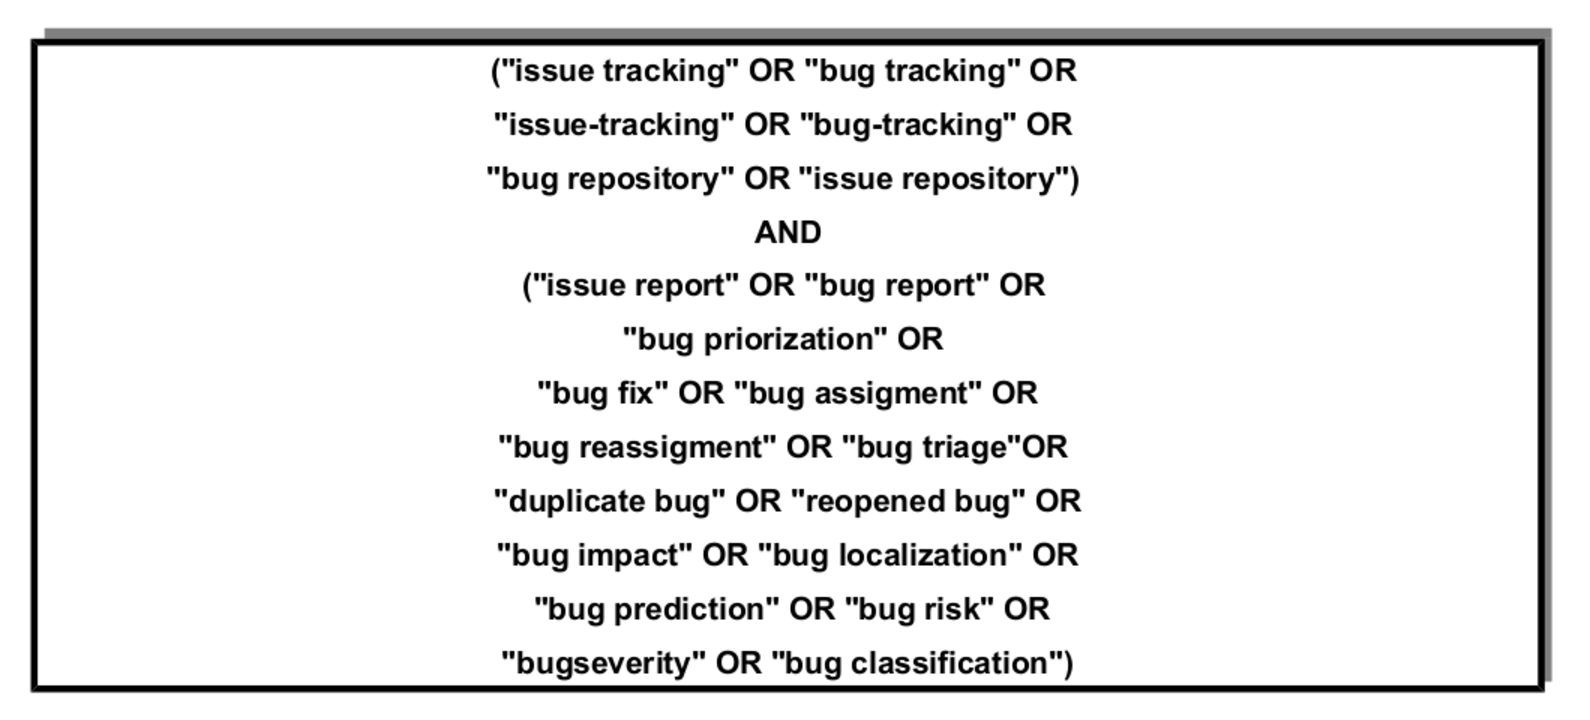
\includegraphics[width=0.8\linewidth]{./chapter-pesquisa-com-profissionais/img/setencas-grupos.pdf}
	\caption{Sentenças utilizadas para escolhas dos grupos do LinkedIn e de
		discussões no Stack Overflow}
\label{fig:setencas-grupos}
\end{figure}

\subsubsection{Estratégia de Amostragem}
\label{subsubsec:pesquisa_profissionais_estrategia_amostragem}

Apesar das Fontes de Amostragens terem sido extraídas de diferente locais, pode
ocorrer uma sobreposição de participantes, ou seja, alguém do projeto Python
pode ter participado determinada discussão no Stack Overflow. Para minimizar a
possibilidade da duplicação de participação de uma mesma unidade de observação
realizamos uma  desenho de amostragem conhecido como Agrupada. Uma Amostragem
agrupada pode ser aplicada quando grupos homogêneos (clusters) compostos por
unidades distintas podem ser identificados numa população. Como consequência,
devido a essa similaridade, apenas um subconjunto desta população pode ser
utilizado como amostra de forma aleatória, sem perda significativa de
confiança~\cite{thompson2012sampling}. Assim, a amostragem em agrupamentos é
comumente aplicada em pesquisas em larga escala nas quais os pesquisadores têm
restrições operacionais para recrutar e coletar
dados~\cite{roberts2004mortality}.

\subsubsection{Extração de Dados}
\label{subsubsec:pesquisa_profissionais_extracao_dados}

Para a extrairmos os dados da rede social Stack Overflow utilizamos sua
ferramenta web oficial que permite compartilhar, consultar e analisar os dados
de todos os sites da rede Stack
Exchange\footnote{\url{http://data.stackexchange.com/stackoverflow}}. A
ferramenta possibilita a utilização da linguagem SQL para acesso aos dados. A
Figura~\cite{fig:stack-exchange}. É possível ainda extrair os dados formato CSV
(Comma Separated Values) o qual foi posteriormente inserido em um banco de dados
para aplicação das regras de inclusão e exclusão.

\begin{figure}[htpb]
	\centering
	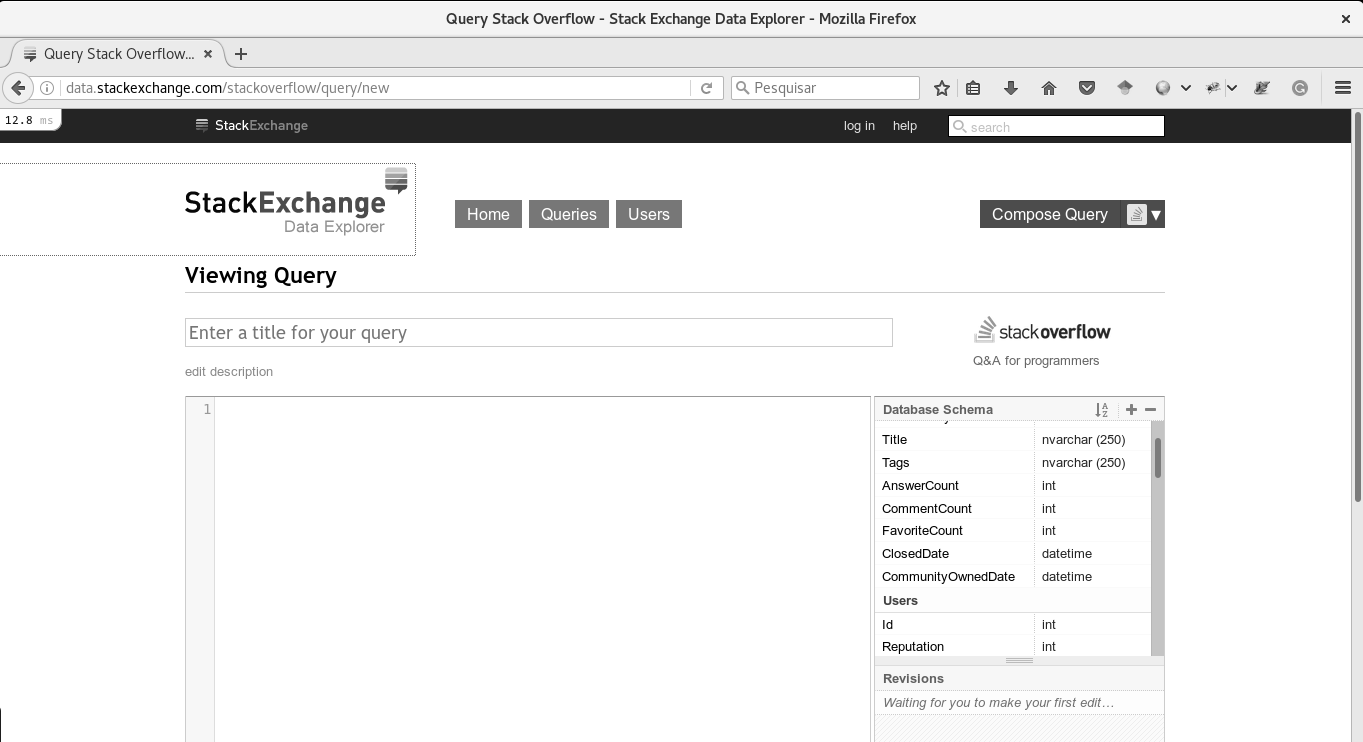
\includegraphics[width=0.8\linewidth]{./chapter-pesquisa-com-profissionais/img/stack-exchange.png}
	\caption{Ferramenta de coleta de dados da rede Stack Overflow}
\label{fig:stack-exchange}
\end{figure}

Para o projeto de código aberto foi desenvolvido um Web Crawler para coletar as
informações dos participantes. Um Web Crawler (rastreador web) é um programa de
computador que navega pela World Wide Web de uma forma metódica e automatizada.
A partir de uma lista de RMs previamente coletadas a ferramenta coletou os dados
dos participantes a partir do histórico de modificações da mesma. A
Figura~\cite{fig:historico-rm-python} apresenta o histórico de registros de uma
RM do projeto Python onde os dados dos participantes podem ser visualizados nos
quadros inseridos. A ferramenta utiliza uma marcação HTML e os seu valor de
classe (título, ou seja, nome de membro) para coletar os dados. Os dados
coletados também foram armazenadas em um banco de dados para posterior aplicação
de critérios de inclusão e exclusão.

\begin{figure}[htpb]
	\centering
	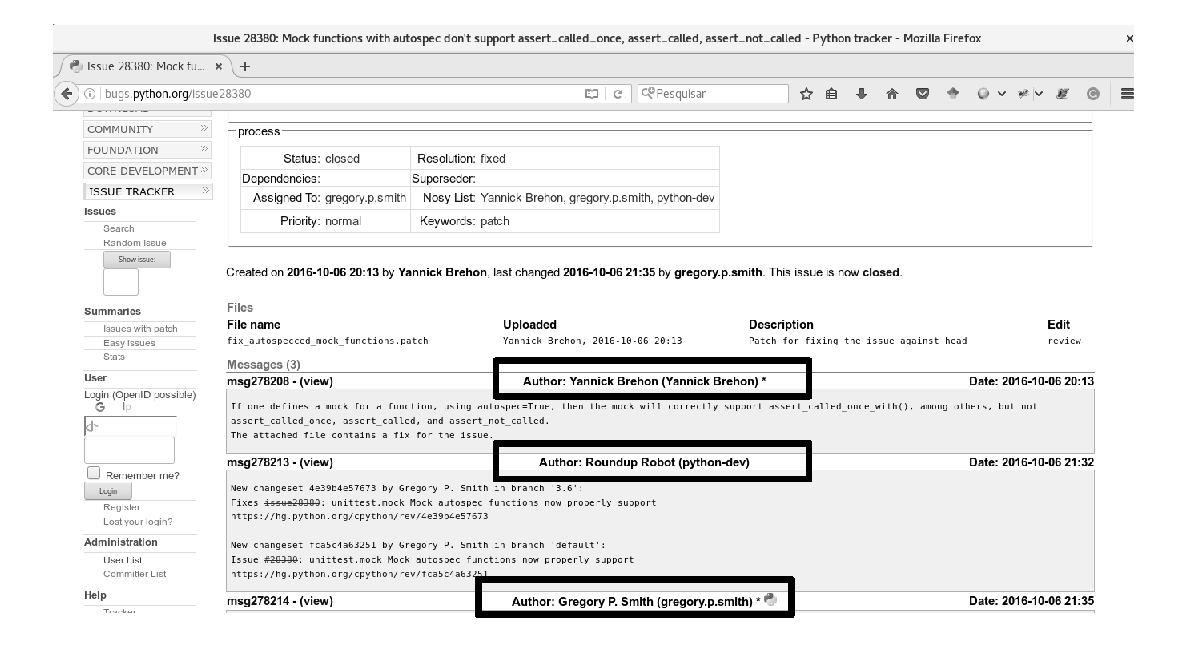
\includegraphics[width=0.6\linewidth]{./chapter-pesquisa-com-profissionais/img/historico-rm-python.pdf}
	\caption{Histórico de relatos de uma RM do projeto Python}
\label{fig:historico-rm-python}
\end{figure}

\subsubsection{Questionário}
\label{subsec:questionario}

O formulário enviado aos participantes foi estruturado em três parte, cada uma
com o objetivo de coletar um conjunto distinto de informações. Na primeira parte
estamos interessados na formação de base (background) dos profissionais. O
segundo conjunto de perguntas visa obter a percepção dos participantes sobre as
funcionalidades atualmente oferecidas pelas FGRM\@. A terceira parte é do
formulário contêm as perguntas sobre a percepção dos participantes sobre as
extensões propostas na literatura.

A fim de obtermos um formulário que conseguisse atingir os objetivos deste
estudo, realizamos um processo de avaliação em quatro etapas. O formulário
resultante de uma etapa anterior foi utilizado como entrada de uma etapa
posterior. Desta forma, utilizamos um processo iterativo para produzirmos o
formulário.
\begin{enumerate}[(i)]
	\item Avaliação por Pesquisadores: Nesta etapa o formulário inicialmente
		proposto foi enviado para dois pesquisadores experientes na área de
		manutenção de software.
	\item Avaliação por Profissionais O formulário resultante da análise
		anterior foi encaminhado a dois profissionais experientes envolvidos com
		manutenção de software.
	\item Piloto da Pesquisa O formulário obtido após a fase anterior foi
		utilizado em um piloto com
		dez profissionais envolvidos da manutenção de software de uma empresa
		pública de
		informática~-~PRODABEL\footnote{\url{{http://www.prodabel.pbh.gov.br}}}
	\item Tradução do Formulário Em cada uma das etapas de anteriores o
		formulário foi aplicado em
		português, tendo em vista que alguns profissionais envolvidos no
		processo de avaliação não
		ter fluência em língua inglesa, em especial na fase ``Piloto da
		Pesquisa'. Neste sentido, a última etapa  consistiu na tradução do
		formulário para a língua inglesa.  Esta etapa foi conduzida com  o
		suporte de um pesquisador experiente na área de Engenharia de Software.	
\end{enumerate}

\subsubsection{Envio da Mensagem}

A fim de viabilizar e mitigar os riscos operacionais do envio manual de
mensagens ao participantes foi desenvolvido um processo automatizado de envio de
mensagens ao participantes. O processo de envio seguiu uma política que consiste
em enviar uma mensagem ao participante com base em um modelo. Após um um prazo
de dois dias uma mensagem de lembrete. Foi construída uma lista para incluir os
participantes que gostariam de receber lembretes ou de participar da pesquisa de
modo a respeitar a privacidade do desenvolvedor. As mensagens foram preenchidas
(uma a uma) e enviadas através de correio eletrônico para cada um dos
participantes com base no seguinte modelo:

\fbox{\begin{minipage}{\textwidth}
Dear \{\{ nome do participante\}\}\!

I’m Vagner Clementino (\url{homepages.dcc.ufmg.br/~vagnercs}), Master Student at
Federal University of Minas Gerais, Brazil. I’m conducting a research,
supervised by Prof\. Rodolfo Resende \@-\@ \url{homepages.dcc.ufmg.br/~rodolfo}
concerned with improvements in Issue Tracking System. As part of them, we
planned and executed a survey aiming at to reach a large-scale population of
researchers/practitioners interested on to improve the features of the Issue
Tracking Systems. Based on your area of interest, we kindly invite you to take
part in the following survey:

\{\{url do formulario\}\}

You was chosen because your relevant participation/contribution in \{\{nome da
fonte de amostragem\}\}\@-\@ \{\{url da fonte de amostragem\}\}. Your opinion is
essential to strength our findings. Please, help us accordingly your
possibilities by answering this survey until \{\{data limite\}\}. As soon as we
conclude data analysis, we will share the results with all participants and the
software engineering community. If you have already fulfilled this
questionnaire, please ignore this email.

Thanks in advance,\\
Vagner Clementino\\

\end{minipage}}

\section{Resultados}
\label{sec:analise_dados}

Neste seção apresentamos os resultado obtidos da aplicação do questionário. Os
foram divididos pela questão de pesquisa ao qual visa responder. Começamos com
análise do perfil dos respondentes. Em seguida, avaliamos o nível de satisfação
que os participantes possuem com as ferramentas que eles utilizam.
Posteriormente verificamos a adoção das metodologias propostas pelos agilistas
no processo de desenvolvimento e manutenção de software. 
%Por se tratar de um estudo exploratório, no qual não foi proposta determinada
%tese a ser provada, a análise dos resultados é feita mediante o uso de gráficos
%representando a escala de Likert. Este tipo de grafo é recomendado para
%visualizar dados na escala de Likert tendo em vista que possibilita o
%entendimento da divergência entre as respostas dos
%participantes~\cite{robbins2011plotting}

\subsection{Perfil dos Participantes}
\label{sub:pesquisa_prof_perfil_dos_participantes}

Antes de apresentamos os resultado sobre as ferramentas, avaliamos o perfil dos
respondente do questionário. Como pode ser observado na
Figura~\ref{fig:grafico_melhorias_fgrm_funcao_particantes} a função mais
frequente é a de desenvolvedor. Todavia grande parte dos respondentes estão
diretamente vinculado ao desenvolvimento e manutenção de software, tanto que
mais de 80\% é formado por desenvolvedores, engenheiros de software, gerentes e
arquitetos. 

\begin{figure}[htpb]
	\centering
	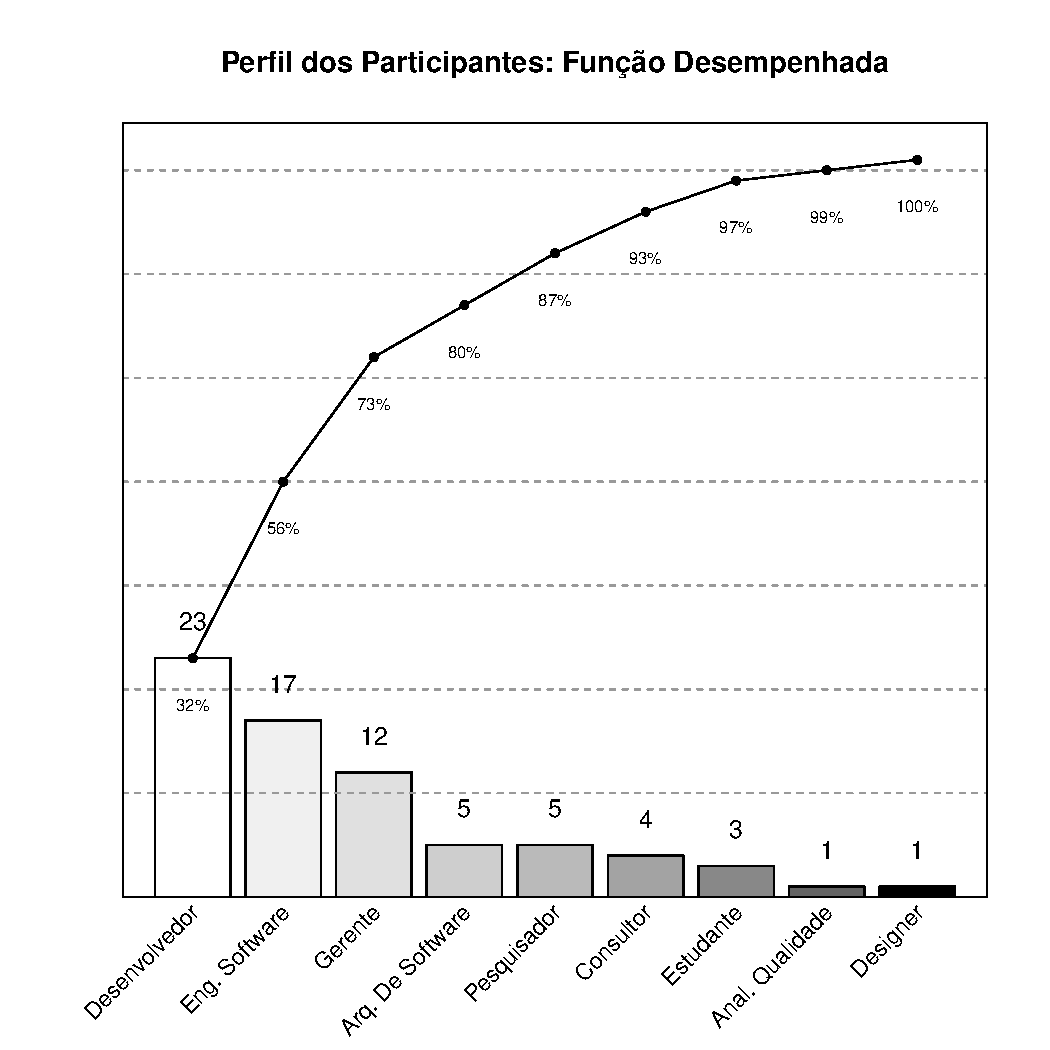
\includegraphics[width=0.8\linewidth]{./chapter-pesquisa-com-profissionais/img/grafico_melhoria_fgrm_funcao_participantes.pdf}
	\caption{Função dos Participantes}
\label{fig:grafico_melhorias_fgrm_funcao_particantes}
\end{figure}

A distribuição geográfica dos participantes pode ser visualizada na
Figura~\ref{fig:grafico_melhorias_fgrm_localizacao_geografica}. Há uma
proeminência de pessoas da Ásia e Europa e posteriormente das Américas. Esta
distribuição pode minimizar possíveis enviesamentos que por ventura algum nicho
geográfico possa apresentar. Todavia, não está no escopo deste estudo discutir
as diferenças que a localização do participante influencia aos resultados. 

\begin{figure}[htpb]
	\centering
	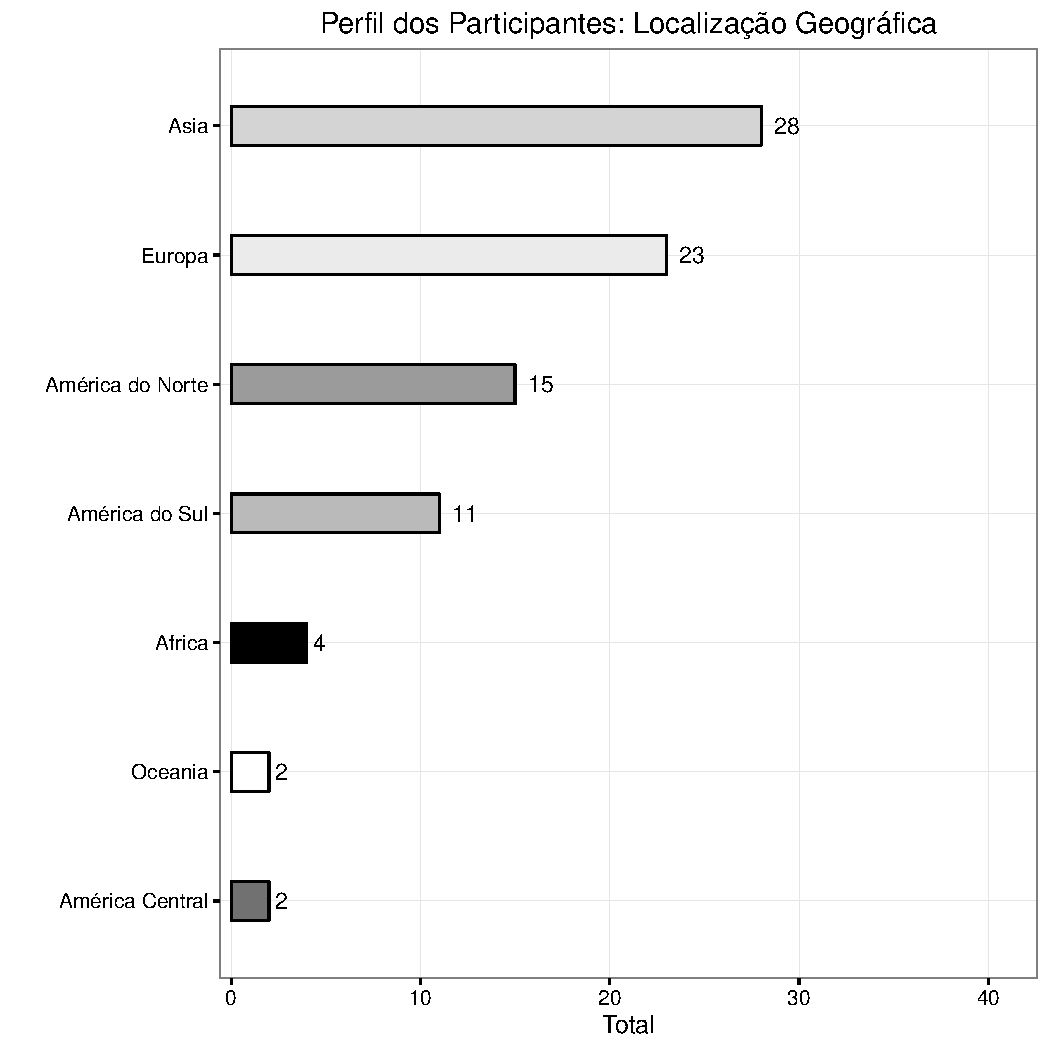
\includegraphics[width=0.8\linewidth]{./chapter-pesquisa-com-profissionais/img/grafico_melhorias_fgrm_localizacao_geografica.pdf}
	\caption{Localização Geográfica dos Participantes}
\label{fig:grafico_melhorias_fgrm_localizacao_geografica}
\end{figure}

Os respondentes trabalham em sua maioria em empresas privadas de software.
Existem também aqueles que participam de projetos de código aberto. A
distribuição do local do participante pode ser vista na
Figura~\cite{fig:grafico_melhorias_fgrm_local_trabalho}. É importante considerar
que grande parte dos respondentes pertencem à empresas privadas, onde os
processos e ferramentas não podem ser modificados pelo desenvolvedor. Esta
característica dos participantes pode afetar os resultados, especialmente quando
	avaliarmos o nível de satisfação com as FGRMs. 

\begin{figure}[htpb]
	\centering
	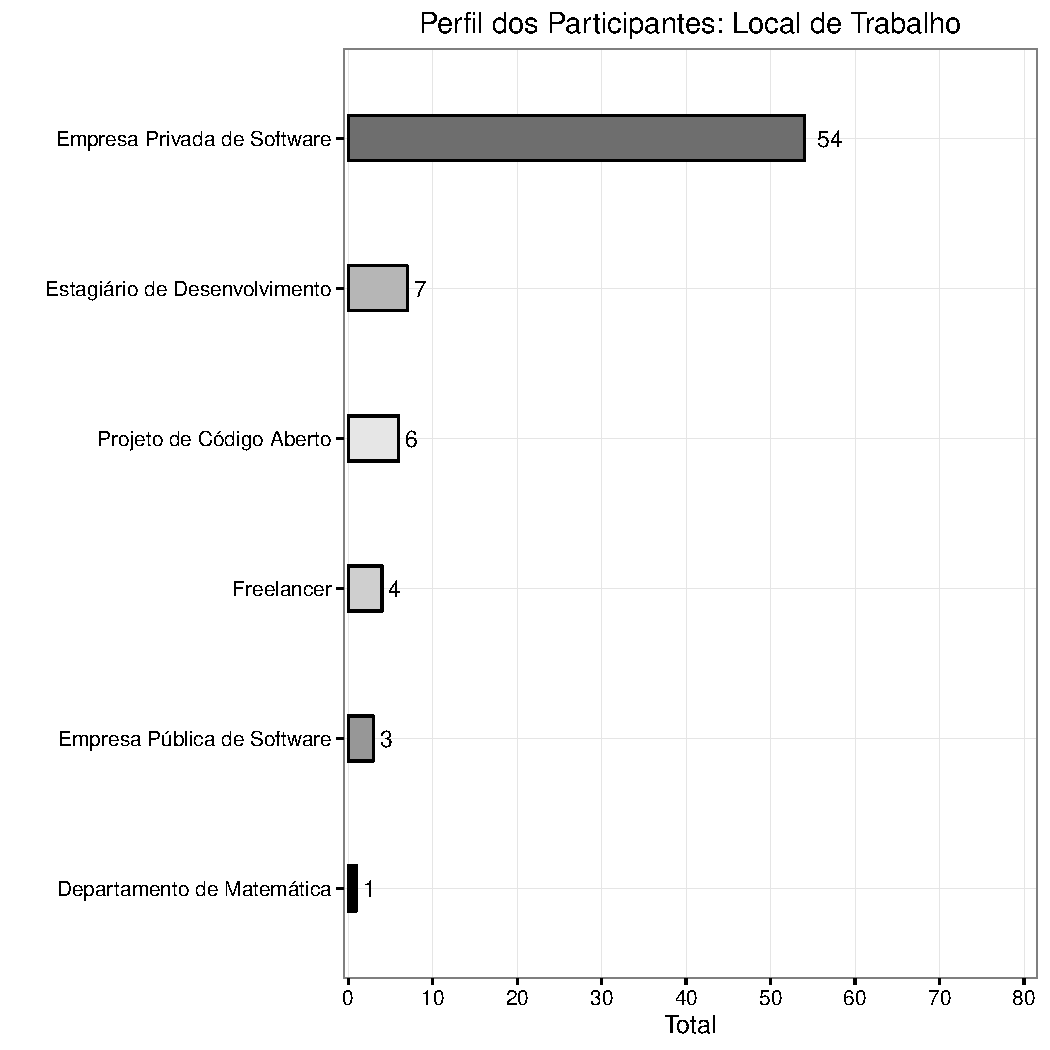
\includegraphics[width=0.8\linewidth]{./chapter-pesquisa-com-profissionais/img/grafico_melhorias_fgrm_local_trabalho.pdf}
	\caption{Local de Trabalho}
\label{fig:grafico_melhorias_fgrm_local_trabalho}
\end{figure}

No tocante ao tamanho da equipe ao qual o participante faz parte verificamos a
predominância de um número com mais de seis membros, conforme pode ser observado
na Figura~\ref{fig:grafico_melhorias_fgrm_tamanho_equipe}. Apesar da maior
frequência de respostas é para equipes de tamanho maior do que dez membros,
acreditamos que o número de membros não seja muito maior do que isso.

\begin{figure}[htpb]
	\centering
	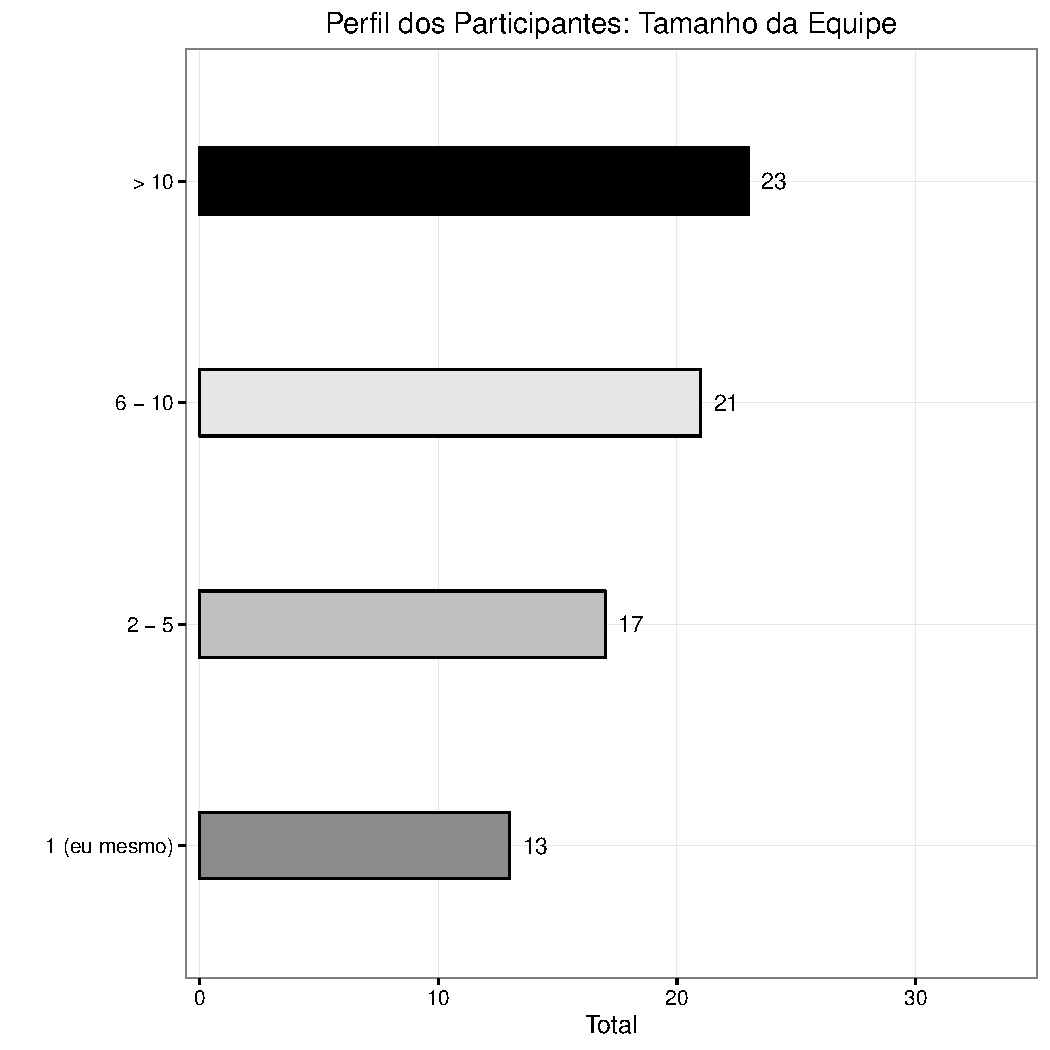
\includegraphics[width=0.8\linewidth]{./chapter-pesquisa-com-profissionais/img/grafico_melhorias_fgrm_tamanho_equipe.pdf}
	\caption{Tamanho da Equipe}
\label{fig:grafico_melhorias_fgrm_tamanho_equipe}
\end{figure}

Os participantes possuem com maior frequência entre três e dez anos. Existem
ainda um grupo significativo (09 participantes) que possuem mais de dez anos de
experiência. Em síntese, temos um grupo com significativa experiência o que pode
agregar valor aos resultados finais. A distribuição do tempo de experiência pode
ser visualizado na Figura~\ref{fig:grafico_melhorias_fgrm_tempo_experiencia}.

\begin{figure}[htpb]
	\centering
	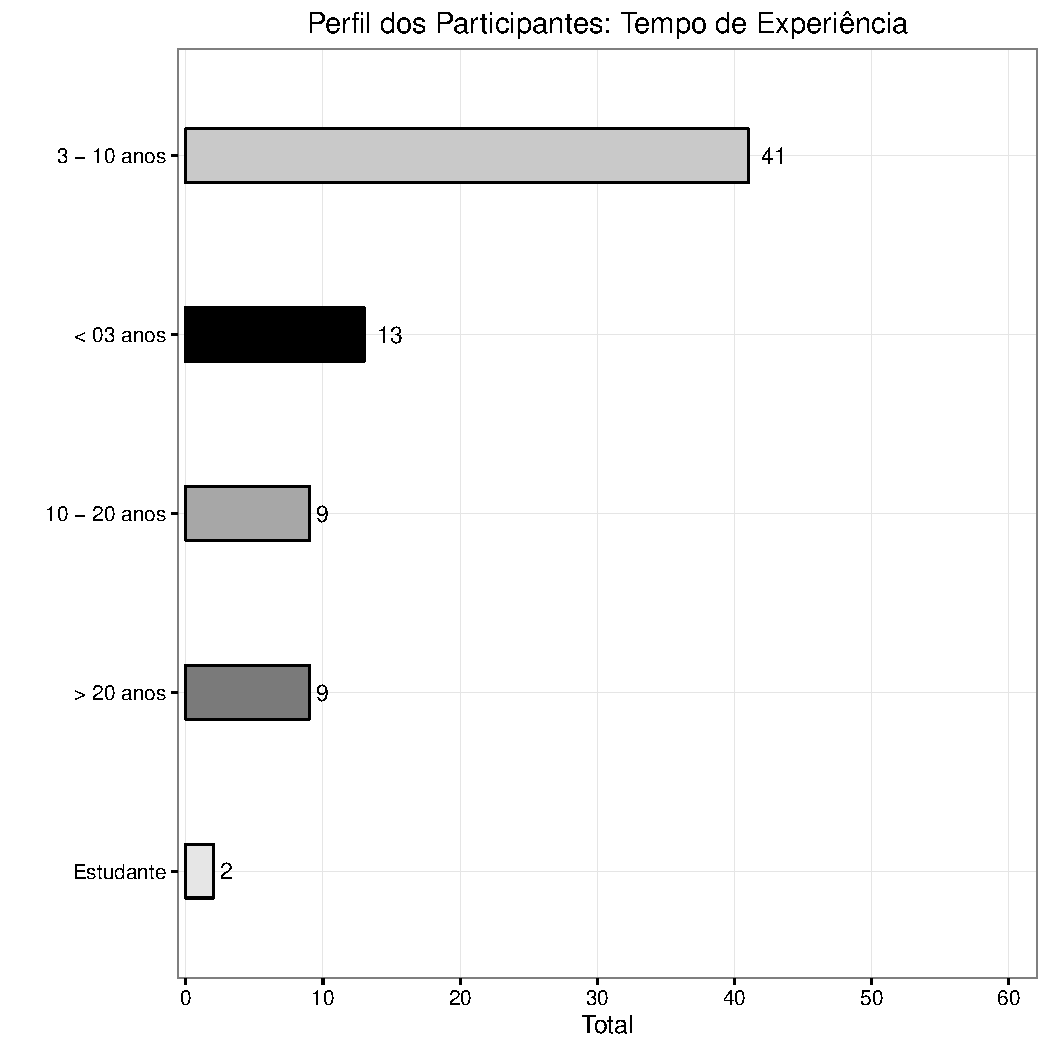
\includegraphics[width=0.8\linewidth]{./chapter-pesquisa-com-profissionais/img/grafico_melhorias_fgrm_tempo_experiencia.pdf}
	\caption{Tempo de Experiência}
\label{fig:grafico_melhorias_fgrm_tempo_experiencia}
\end{figure}

Em resumo as respostas vieram de desenvolvedores, localizados na Ásia e Europa,
com um tempo de experiência entre três e dez anos, trabalhando em uma equipe com
aproximadamente dez membros. A partir deste perfil entendemos que conseguimos
alcançar uma amostra com um perfil suficiente para responder as questões
propostas.

\subsection{Nível de Satisfação com as FGRM}
\label{sub:nivel_de_satisfação_com_as_fgrm}

Para respondermos a Questão de Pesquisa é importante analisarmos as ferramentas
utilizadas pelos profissional que respondeu a pesquisa. Esta informação é
importante tendo que vista que as opiniões dadas pelos participantes estão
diretamente relacionada com a versão utilizada, podendo os resultados se
mostrarem diferentes se a pesquisa fosse realizada com outra versão dos sistema.
A Figura~\ref{fig:grafico_melhorias_fgrm_ferramentas_utilizadas} exibe as
ferramentas utilizadas pelos profissionais que responderam ao questionário. A
maior frequência na ferramenta \textit{Jira} que é uma FGRM que integra em seu
processo de gestão das RMs métodos propostos pelos agilistas. Na segunda
posição visualizamos o Github que é um serviço de web para armazenamento para
projetos que usam o controle de versionamento \textit{Git} e possui uma FGRM
integrada.

\begin{figure}[htpb]
	\centering
	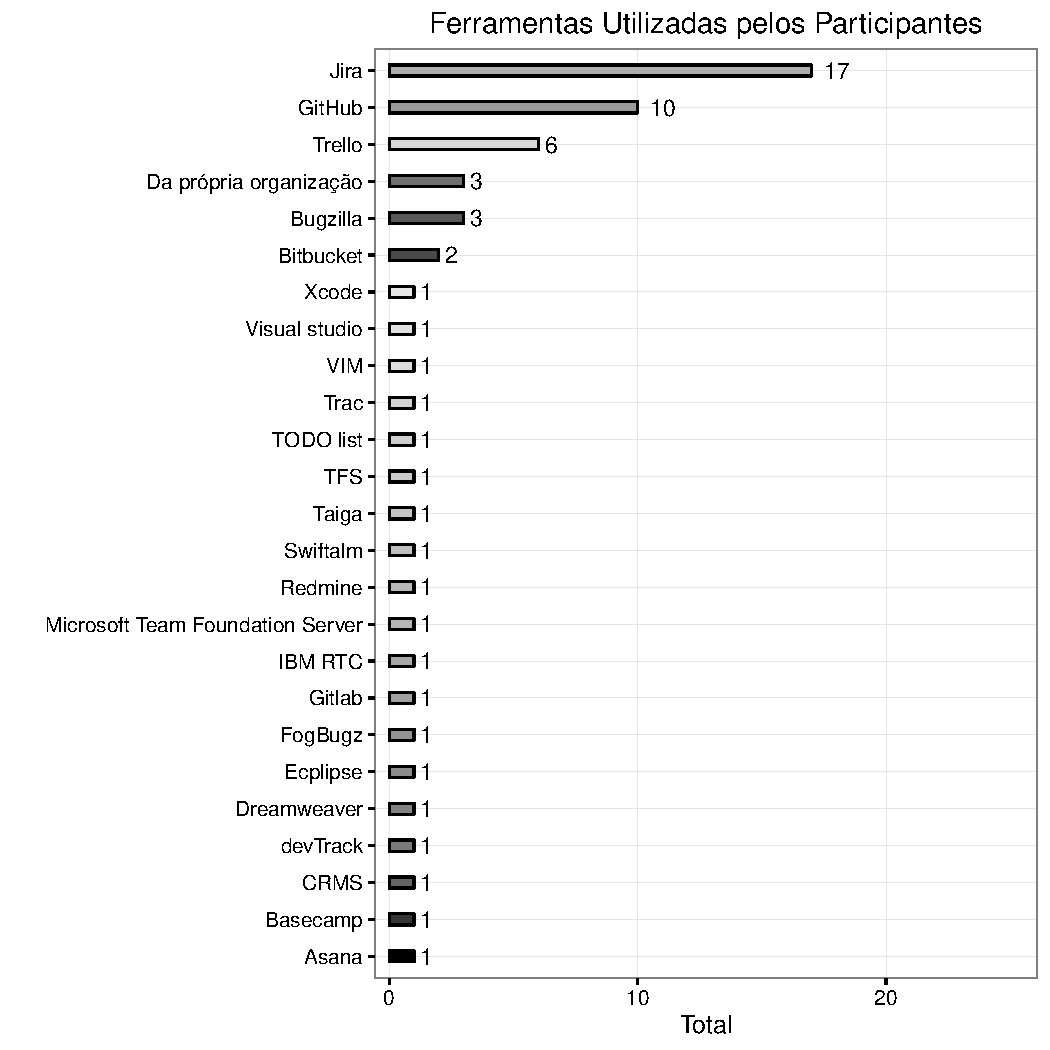
\includegraphics[width=0.8\linewidth]{./chapter-pesquisa-com-profissionais/img/grafico_melhorias_fgrm_ferramentas_utilizadas.pdf}
	\caption{Ferramentas utilizadas pelos participantes}
\label{fig:grafico_melhorias_fgrm_ferramentas_utilizadas}
\end{figure}

Inicialmente gostaríamos de saber qual o nível de satisfação com os participantes
com as funcionalidades pelas FGRM que ele utiliza atualmente. Esta medida pode
ser visualizada na Figura~\ref{grafico_melhorias_fgrm_nivel_satisfacao}. Em
grande parte os respondentes estão satisfeitos com as funcionalidades. A
resposta com maior frequência foi \textit{OK}, o que pode ser visto que este
tipo de software está atualmente atendendo as expectativas de seus usuários.
Este resultado não segue o que literatura da área discute, onde este tipo de
ferramenta é vista com necessidade de melhora, tomando com base a visão dos
profissionais. Esta aparente dicotomia pode ser justificada, possivelmente, pelo
desconhecimento dos profissionais de funcionalidades que estão sendo propostas
na literatura que podem melhorar as suas atividades diárias.
\begin{figure}[htpb]
	\centering
	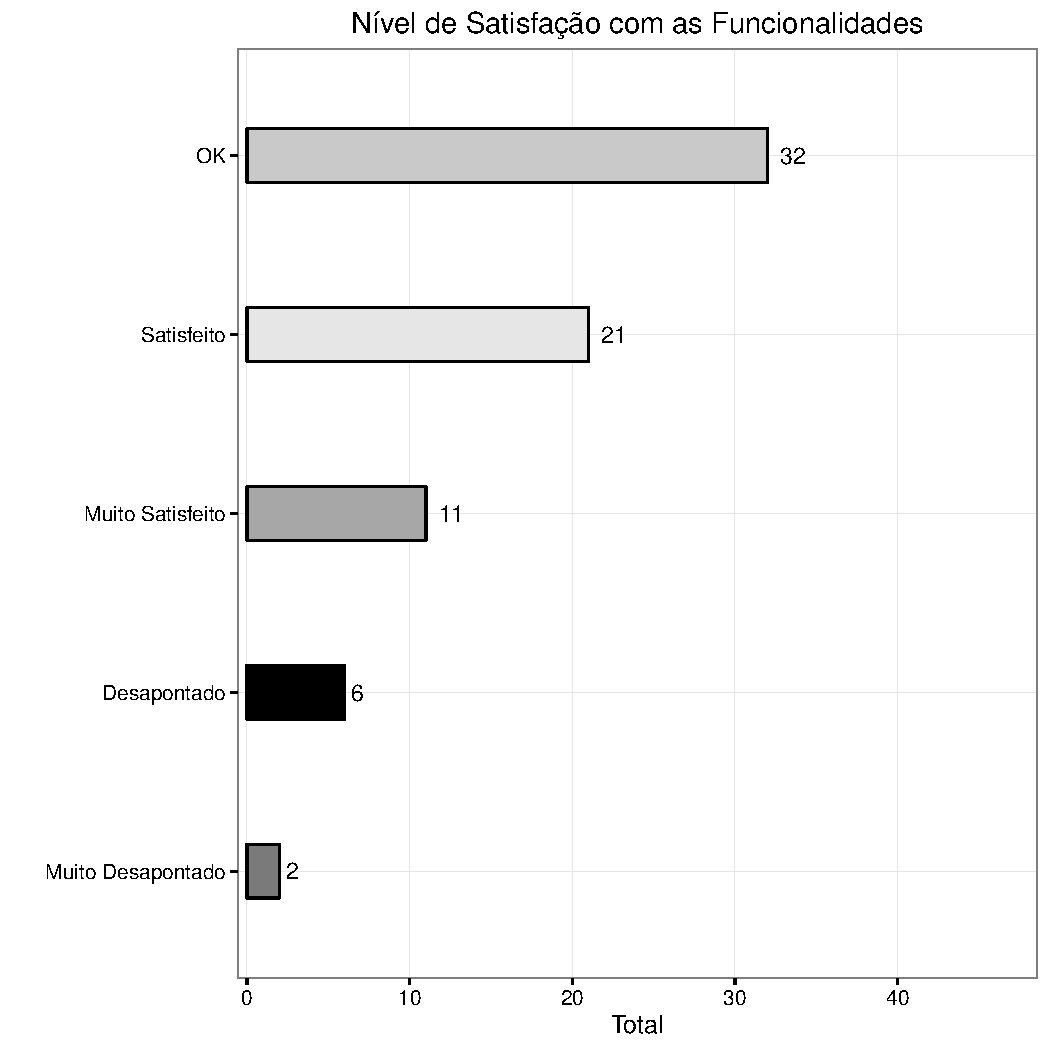
\includegraphics[width=0.8\linewidth]{./chapter-pesquisa-com-profissionais/img/grafico_melhorias_fgrm_nivel_satisfacao.pdf}
	\caption{Nível de satisfação com as Ferramentas}
\label{fig:grafico_melhorias_fgrm_nivel_satisfacao}
\end{figure}

No mesmo questionário verificamos junto aos profissionais se eles recomendariam
a ferramenta que utiliza atualmente para um outro projeto. A probabilidade de
recomendação é exibida na
Figura~\ref{fig:grafico_melhorias_fgrm_probabilidade_recomentacao}. De maneira
similar ao nível de satisfação grande parte dos participantes tendem a
recomendar a FGRM que utiliza para um novo projeto. Com base neste resultado
podemos deduzir que os profissionais estão realmente satisfeitos comas
funcionalidades da ferramenta que utiliza ao ponto de recomendá-la.

\begin{figure}[htpb]
	\centering
	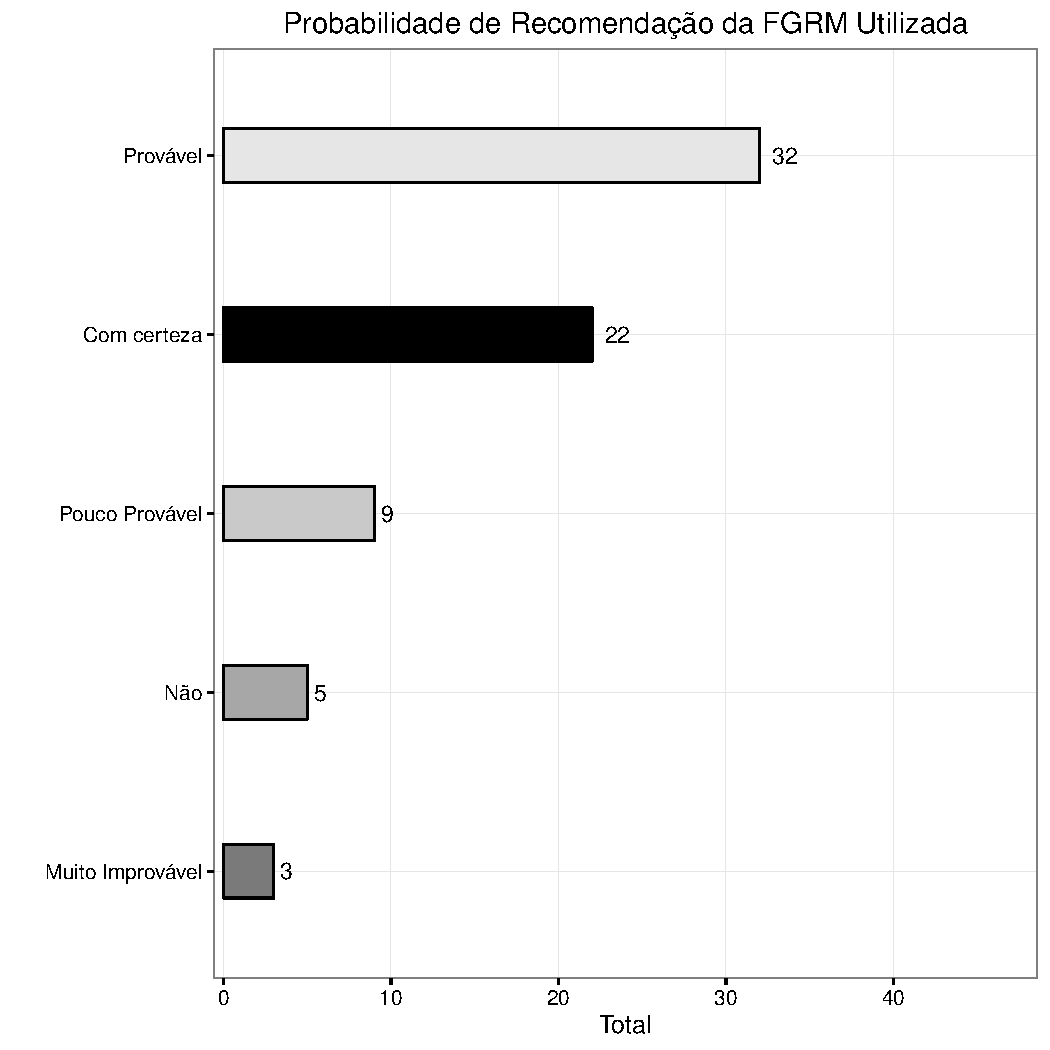
\includegraphics[width=0.8\linewidth]{./chapter-pesquisa-com-profissionais/img/grafico_melhorias_fgrm_probabilidade_recomentacao.pdf}
	\caption{Probabilidade de Recomendação da Ferramenta Utilizada}
\label{fig:grafico_melhorias_fgrm_probabilidade_recomentacao}
\end{figure}

\subsection{Avaliação das Funcionalidades Existentes}
\label{sub:avaliação_das_funcionalidades_existentes}

Nesta seção apresentamos a opinião dos profissionais envolvidos em Manutenção de
Software com relação as funcionalidades oferecidas atualmente pelas FGRM\@. Este
ponto de vista pode ser visualizado na
Tabela~\ref{tab:avaliacao_funcionalidades}. É possível verificar que os
profissionais avaliaram como importantes funções como \textit{Suporte ao
	Unicode, Múltiplos Projetos, Integração com Sistemas de Controle de Versão
	(VCS Integration)} como  funções importantes em sua atividades diárias. 

\begin{table}[htpb]
\centering
\resizebox{\textwidth}{!}{%
\begin{tabular}{@{}|l|ccccc|@{}}
\toprule
\multicolumn{1}{|c|}{\multirow{2}{*}{\textbf{Funcionalidade}}} & \multicolumn{5}{c|}{\textbf{Classificação}} \\ \cmidrule(l){2-6}
\multicolumn{1}{|c|}{} & \multicolumn{1}{c|}{\textbf{Not at all important}} & \multicolumn{1}{c|}{\textbf{Slightly Important}} & \multicolumn{1}{c|}{\textbf{Important}} & \multicolumn{1}{c|}{\textbf{Fairly Important}} & \textbf{Very Important} \\ \midrule
Documentation integration/generation, business reporting & 11 & 12 & 15 & 12 & 14 \\
Test planning integration & 11 & 13 & 13 & 13 & 9 \\
Customizable workflow & 9 & 14 & 21 & 14 & 15 \\
Unicode support & 9 & 9 & 21 & 16 & 24 \\
Custom fields & 5 & 17 & 25 & 22 & 8 \\
Support to Service Level Agreement & 14 & 22 & 15 & 13 & 10 \\
Plugin API to integration with other products & 8 & 14 & 21 & 19 & 16 \\
Multiple projects & 3 & 8 & 17 & 21 & 28 \\
Full-text search & 1 & 5 & 17 & 15 & 40 \\
File search & 4 & 15 & 18 & 17 & 24 \\
VCS integration & 7 & 16 & 16 & 13 & 21 \\
Multiples interfaces of notifications (E-mail, RSS, XMPP, etc) & 7 & 11 & 23 & 16 & 19 \\
Code Review Support & 2 & 2 & 0 & 0 & 5 \\
Ease of use & 0 & 2 & 2 & 0 & 1 \\
Integration with database \& app & 4 & 6 & 4 & 1 & 2 \\
Reviewing & 0 & 4 & 10 & 6 & 1 \\
User Experience and Ease of Use & 2 & 4 & 0 & 6 & 3 \\
Git branch style & 10 & 2 & 2 & 3 & 2 \\ \bottomrule
\end{tabular}%
}
\caption{My caption}
\label{my-label}
\end{table}

Por outro apresentamos aos profissionais funcionalidades que poderiam ser
integradas à FGRM que ele utiliza. A opinião dos participantes pode ser
visualizada na Figura~\ref{fig:ggrafico_melhorias_fgrm_melhorias}. Conforme pode
ser observado que melhorias na busca de busca de RMs, coleta de informações
para solucionar na resolução da RM e dar suporte ao registro de RMs como
funcionalidades que podem melhorar as atividades do desenvolvedor.

\begin{figure}[htpb]
	\centering
	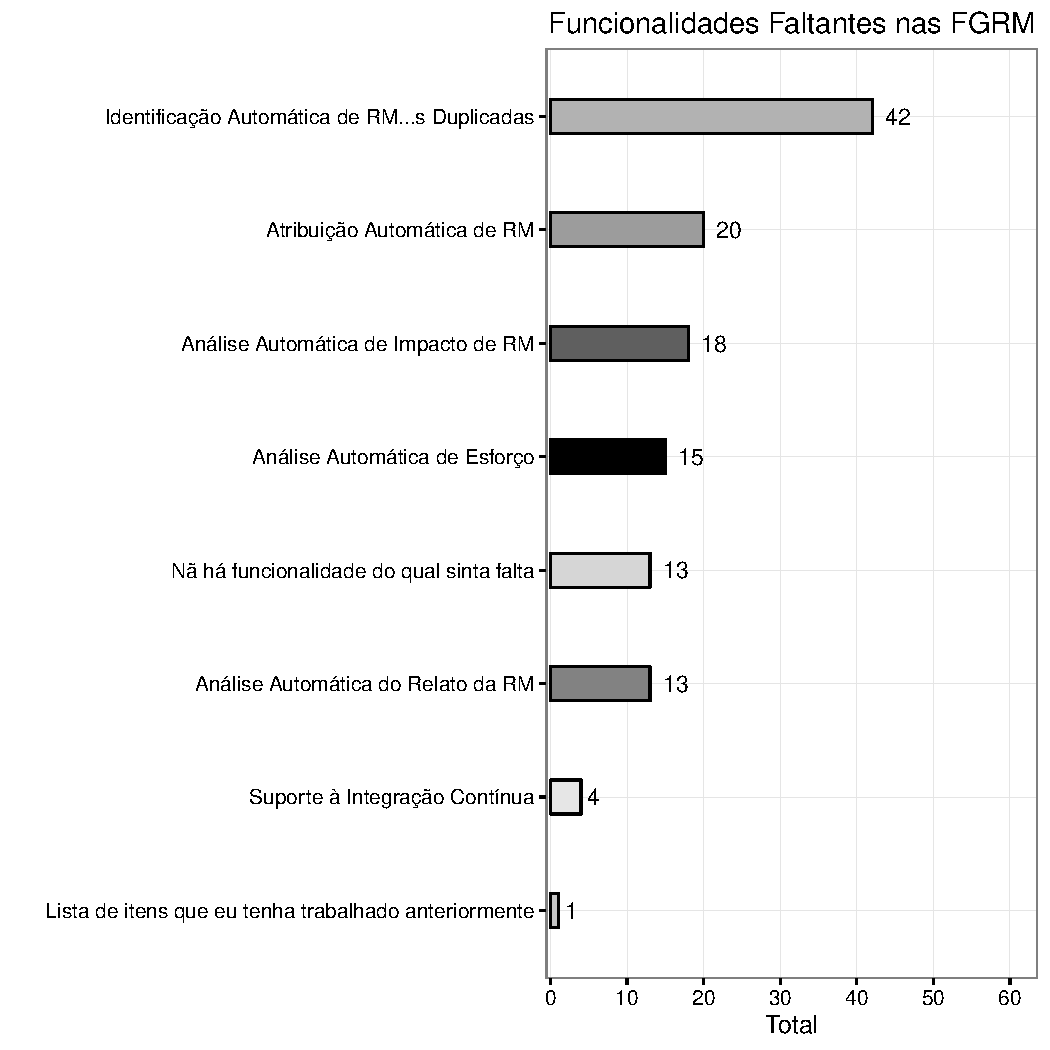
\includegraphics[width=0.8\linewidth]{./chapter-pesquisa-com-profissionais/img/grafico_melhorias_fgrm_funcionalidades_faltantes.pdf}
	\caption{Funcionalidades que o participantes sentem falta.}
\label{fig:grafico_melhorias_fgrm_funcionalidades_falantes}
\end{figure}

Por outro lado algumas das melhorias propostas na literatura se mostram de
interesse pelos profissionais. A
Figura~\ref{fig:grafico_melhorias_fgrm_funcionalidades_falantes} apresenta as
funcionalidades que os participantes sentem falta. Funções tais como
identificação automática de RMs duplicadas, atribuição automática de RM e
Análise de Impacto foram as mais frequentes. 

\begin{figure}[htpb]
	\centering
	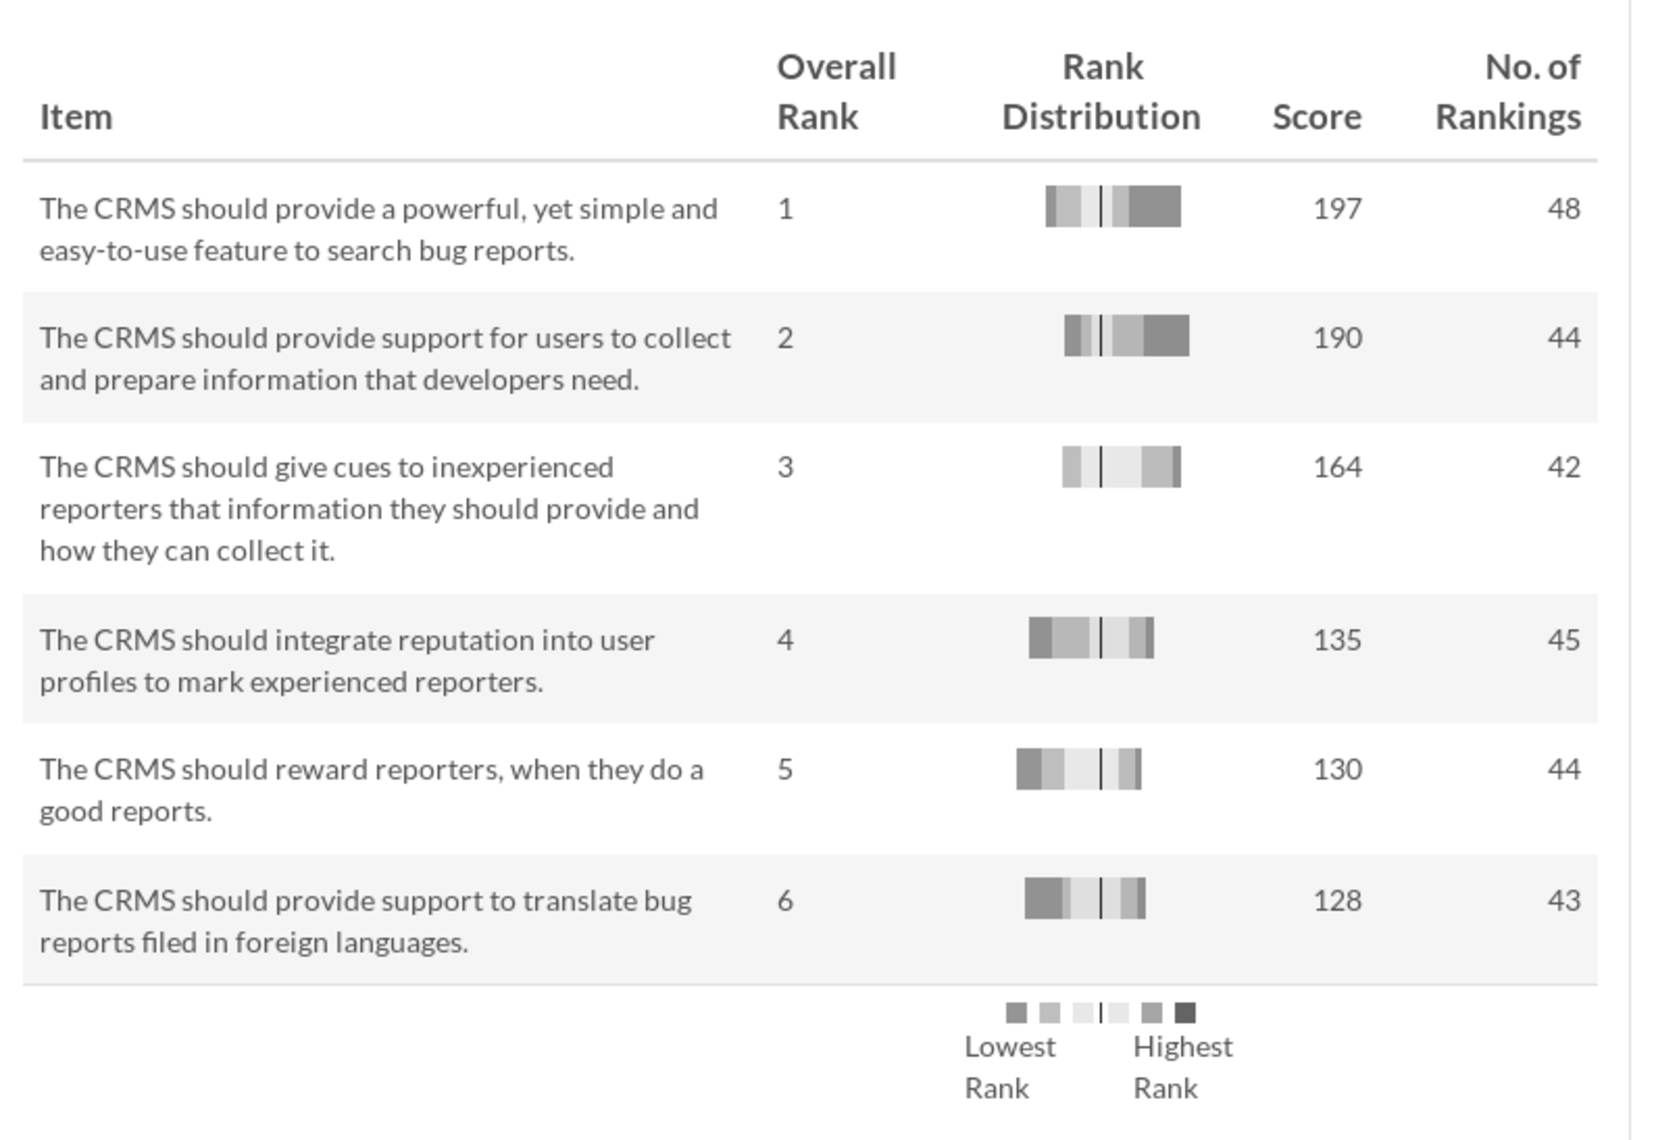
\includegraphics[width=0.8\linewidth]{./chapter-pesquisa-com-profissionais/img/grafico_melhorias_fgrm_melhorias.pdf}
	\caption{Novas funcionalidades para as FGRMs.}
\label{fig:ggrafico_melhorias_fgrm_melhorias}
\end{figure}


\subsection{Práticas Ágeis na Manutenção de Software}
\label{sub:práticas_ágeis_na_manutenção_de_software}

Nesta etapa deste estudos estamos interessados como as práticas propostas pelos
agilistas estão sendo utilizadas especialmente no processo de manutenção de
software. A Figura~\ref{fig:grafico_melhorias_fgrm_praticas_ageis_adotadas}
exibe as metodologias ágeis que estão sendo utilizadas durante o processo de
manutenção de software. As práticas mais adotadas são Integração Contínua,
Padrões de Programação e Refatoração são práticas adotadas quando da realização
desta pesquisa. 

\begin{figure}[htpb]
	\centering
	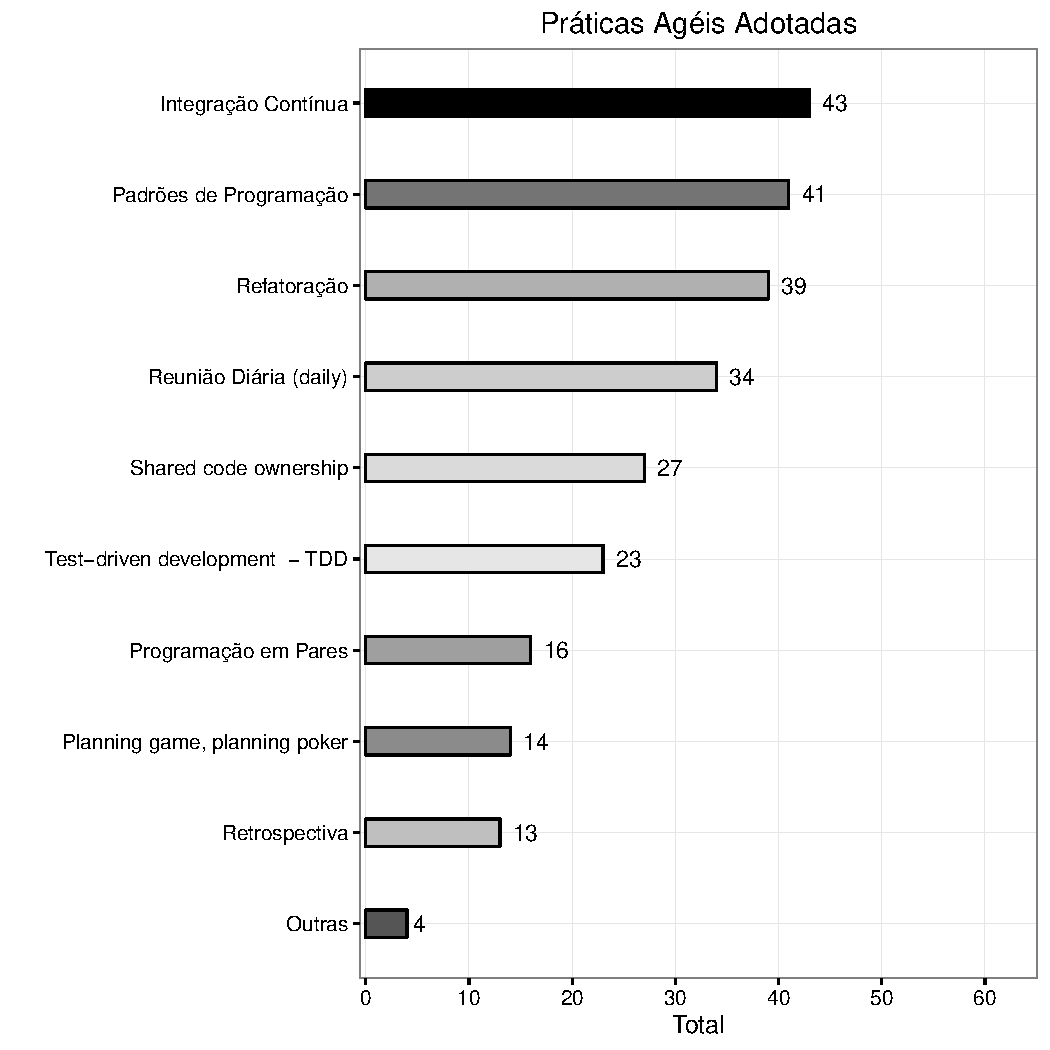
\includegraphics[width=0.8\linewidth]{./chapter-pesquisa-com-profissionais/img/grafico_melhorias_fgrm_praticas_ageis_adotadas.pdf}
	\caption{Metodologias propostas pelos agilistas que são adotadas pelos
		participantes.}
\label{fig:grafico_melhorias_fgrm_praticas_ageis_adotadas}
\end{figure}

A fim de avaliar como as FGRMs podem ajudar aos times devotados à manutenção de
software na prática adotada pelos agilistas apresentamos uma lista de possíveis
funcionalidades que este tipo de ferramenta poderia fornecer. A
Figura~\ref{fig:grafico_melhorias_fgrm_suporte_particas_ageis} apresenta a
opinião dos profissionais quais as funcionalidades seriam mais relevantes.
Segundo a opinião dos participantes a priorização automática de RMs urgente e
não esperadas, ajuda do desenvolvedor em sua reunião diária (daily) e o suporte
a tarefas compartilhadas foram as mais frequentes.

\begin{figure}[htpb]
	\centering
	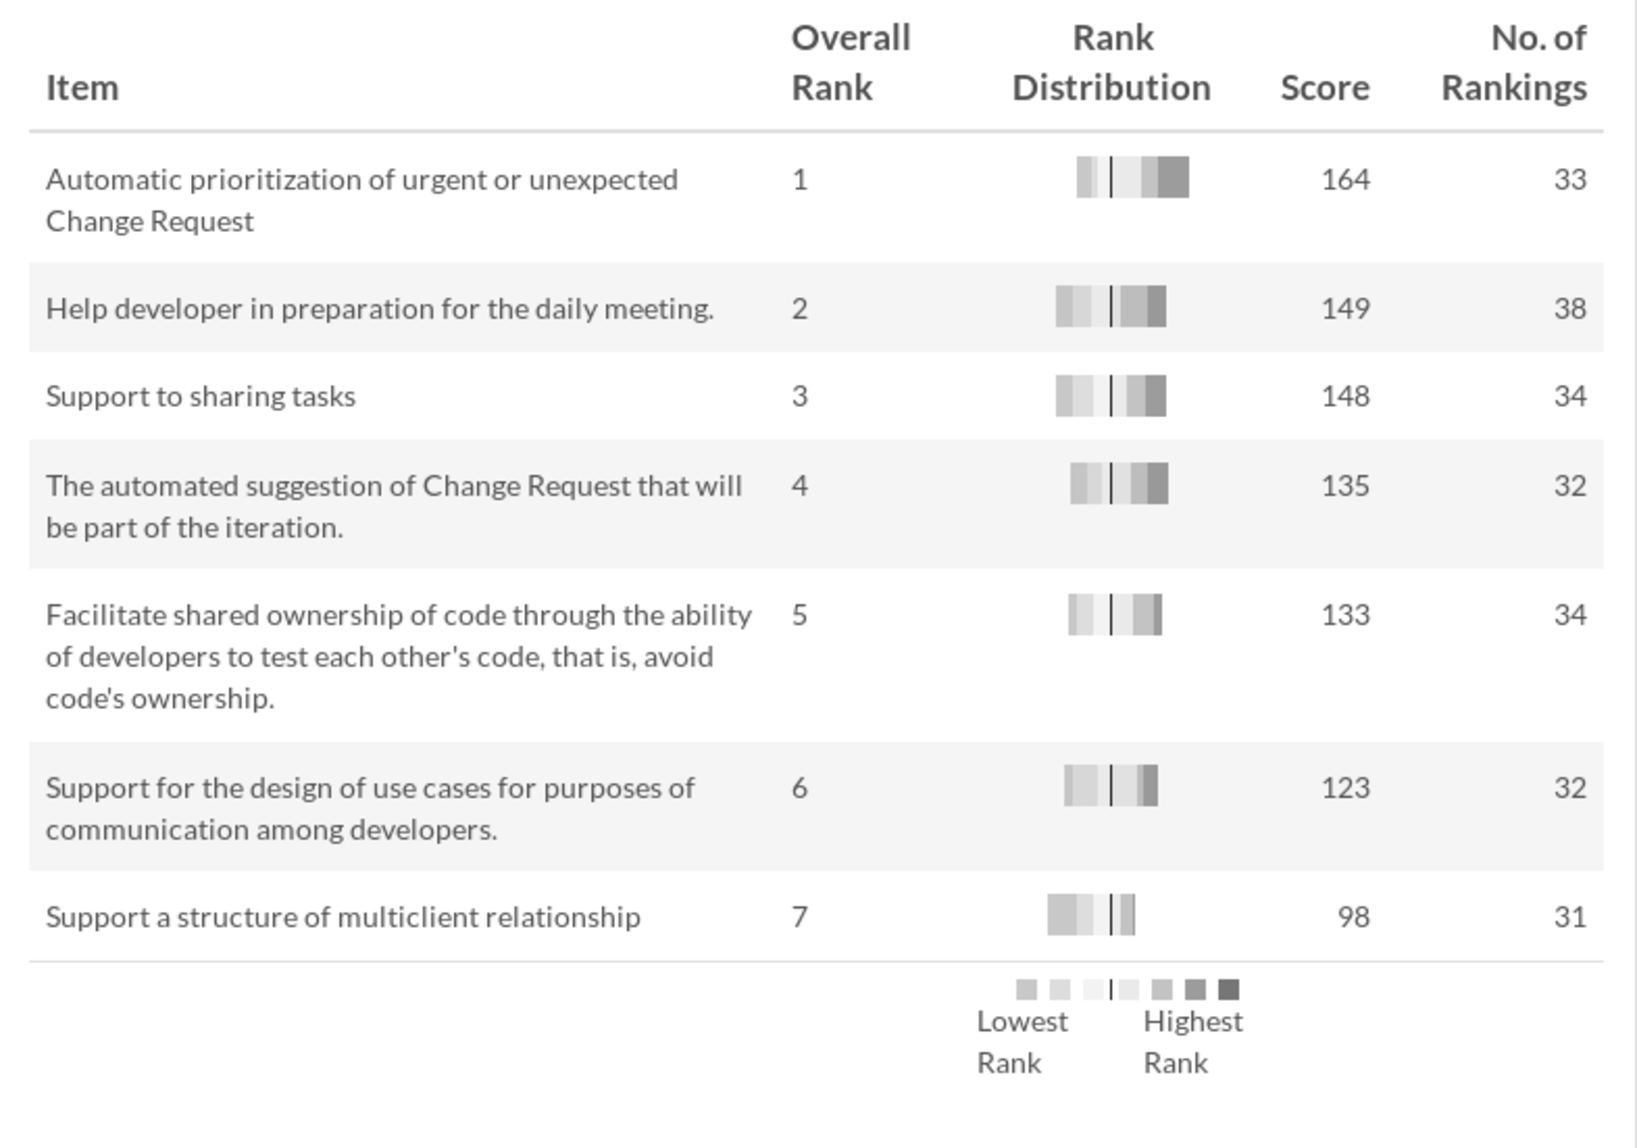
\includegraphics[width=0.8\linewidth]{./chapter-pesquisa-com-profissionais/img/grafico_melhorias_fgrm_suporte_particas_ageis.pdf}
	\caption{Classificação das funcionalidades que possam dar suporte ao uso das
	metodologias dos agilistas.}
\label{fig:grafico_melhorias_fgrm_suporte_particas_ageis}
\end{figure}

\section{Discussão}

\paragraph{Nível de Satisfação com a Ferramenta Utilizada.}
\label{par:pesq_profissionais_nivel_de_satisfação}

Em geral, o nível de satisfação com as funcionalidades oferecidas pelas FGRMs é
alto. Esta medida foi observada no
Figura~\ref{fig:grafico_melhorias_fgrm_nivel_satisfacao} no qual verificamos que
cerca de 90\% dos participantes estão de alguma forma satisfeito com a
ferramenta utilizada diariamente. Este mesmo sentimento pode ser observado pela
probabilidade de recomendação do sistema que utilizada para um novo projeto.
Naquela medida verificamos que o mesmo percentual de participantes pretendem
recomendar o software que utiliza.

\paragraph{Funcionalidades Faltantes.}
\label{par:pesq_profissionais_funcionalidades_faltantes}

\section{Ameças à Validade}
As ameaças à validade deste trabalho está principalmente no numero de
respondentes da pesquisa. Apesar de ter sido realizada uma seleção metodológica
de uma amostra representativa da população o número de participantes limita a
extrapolação do resultados obtidos. Da mesma forma, todas as opiniões coletadas
devem sempre levar em conta a ferramenta que o profissional utilize quando da
aplicação do questionário. Caso este mesmo estudo fosse realizado com outras
versões do mesmos sistemas os resultados poderiam ser diferentes. Neste sentido,
a generalização dos resultados também passa por esta característica do estudo.

\section{Resumo do Capítulo}
\label{sec:resumo_do_capitulo}


%Incluindo o fonte do Capítulo 06
%%%%%%%%%%%%%%%%%%%%%%%%%%%%%%%%%%%%%%%%%%%%%%%%%%%%%%%%%%%%%%%%%%%%%%%%%%%%%%%%
%Objetivo: Propor um conjunto de recomendações de melhorias para as
% 		   as funcionalidade das FGRMs
%Autores: Vagner Clementino <vagnercs@dcc.ufmg.br>
%		  Rodolfo Resende <rodolfo@dcc.ufmg.br>
%Criação: dom fev 26 12:49:27 BRT 2017
%Modificação: qui jul 20 20:46:30 -03 2017
%Revisão: dom abr 23 23:16:51 -03 2017
%%%%%%%%%%%%%%%%%%%%%%%%%%%%%%%%%%%%%%%%%%%%%%%%%%%%%%%%%%%%%%%%%%%%%%%%%%%%%%%%
\chapter{Sugestões de Melhorias para as FGRMs}\label{ch:sug_melhoria}

\section{Introdução}\label{sec:sug_melhoria_intro}

No levantamento por questionário descrito no
Capítulo~\ref{ch:pesquisa-profissionais} os profissionais consultados se
mostraram, em geral, satisfeitos com as funcionalidades disponibilizadas pelas
FGRMs. Cerca de 44\% dos par\-ti\-ci\-pan\-tes fizeram uma avaliação positiva
da ferramenta que utilizam, além disso, também cerca de 76\% dos participantes
disseram que recomendariam as FGRMs que utilizam para um novo projeto (opções
\textit{Provável} e \textit{Com certeza}).

Não obstante, naquela mesma pesquisa, apresentamos uma lista de possíveis novas
funcionalidades para as FGRMs e perguntamos ao participante quais
funcionalidades ele desejaria que fosse incluída  em sua FGRM\@. O resultado
desta pergunta foi que cerca de 85\% se mostraram interessados na inclusão de
pelo menos uma das funções propostas na FGRM que utiliza. A partir da análise
deste resultado é possível inferir que os desenvolvedores estão satisfeitos com
a ferramenta utilizada, contudo, \textit{não conhecem ou não têm acesso ao
    potencial de funcionalidades que este tipo de software pode oferecer}.

Diante do exposto, entendemos que podemos contribuir com o estado a\-tu\-al das
funcionalidades das FGRMs propondo um conjunto de melhorias. As sugestões foram
compiladas utilizando a literatura da área e os levantamentos realizados nesta
dissertação, especialmente com base nos
Capítulos~\ref{ch:mapeamento-sistematico} e~\ref{ch:pesquisa-profissionais}, na
Seção~\ref{sec:caracterizacao_ferramentas} e nos estudos que propõem melhorias
para as FGRM~\cite{zimmermann2009improving, zimmermann2010makes, singh2011bug}.
Estas recomendações podem ser utilizadas por pesquisadores interessados em
conduzir estudos sobre o avanço da produtividade dos desenvolvedores mediante o
uso das FGRMs. Além disso, os responsáveis pelo desenvolvimento deste tipo de
software, podem utilizar algumas das recomendações para a criação ou
aperfeiçoamento das funcionalidades da FGRM pelas quais são responsáveis. Na
mesma linha, os profissionais envolvidos com Manutenção de Software podem criar
extensões (\textit{plug-in}) com base no que foi proposto de modo a aplicar
essas melhorias em sua rotina de trabalho.

Este capítulo está organizado da seguinte forma: a
Seção~\ref{sec:sug_melhoria_melhorando_as_ferraementas} apresenta as sugestões
de melhorias propostas, cada sugestão é seguida de uma breve discussão de como
foi obtida e justificativa de sua consideração; na
Seção~\ref{sec:sug_melhoria_avaliacao_das_melhorias} realizamos uma avaliação do
que foi recomendado com base na opinião de profissionais que contribuem para
projetos relacionados ao desenvolvimento de FGRMs; os resultados do processo de
avaliação são apresentados na
Seção~\ref{sec:resultados_avaliacao_sug_de_melhorias}; na
Seção~\ref{sec:sug_melhoria_discussao} discutimos os resultados obtidos no
processo de avaliação; na Seção~\ref{sec:sug_melhoria_ameacas} apresentamos as
ameaças à validade; encerramos o capítulo com um resumo na
Seção~\ref{sec:sug_melhoria_resumo}.

\section{Sugestões de Melhorias para FGRMs}\label{sec:sug_melhoria_melhorando_as_ferraementas}

As sugestões propostas neste capítulo não estão vinculadas exclusivamente à
melhorias de funcionalidades existentes nas FGRMs. As recomendações podem
representar o desenvolvimento de um novo comportamento ou a melhoria de outros
já existentes. Cabe-nos ressaltar que o conjunto proposto não é exaustivo e é
baseado nos resultados desta dissertação.

É possível que algumas das recomendações propostas já estejam implementadas de
maneira parcial ou integral.  Infelizmente não tivemos como verificar isso em
função do esforço exigido pelo grande volume de ferramentas disponíveis quando
esta dissertação foi escrita. Além disso, o processo de validação descrito na
Seção~\ref{sec:sug_melhoria_avaliacao_das_melhorias} pôde nos alertar sobre a
eventual proposição de uma funcionalidade existente. Ao longo da elaboração das
sugestões verificamos que não conseguiríamos implementá-las e também não
conseguiríamos analisar a complexidade de estratégias de implementação.
Entretanto, como prova de conceito, a sugestão descrita na
Seção~\ref{sub:supote_a_qualidade_do_relato} foi implementada como extensão do
repositório de RMs da plataforma Github, conforme pode ser visto no
Capítulo~\ref{ch:implemtacao_extensao}. As sugestões realizadas foram
estruturadas como seções deste capítulo, em que apresentamos a
\textit{justificativa, o benefício gerado, as limitações e exemplos de
    utilização.}

\subsection{Suporte à Qualidade do Texto Relatado}\label{sub:supote_a_qualidade_do_relato}

\sugestao{01}{As FGRMs devem fornecer realimentação (\textit{feedback})
    relacionado à qualidade do texto relatado.}

\paragraph{Justificativa:}\label{par:justificativa_s01}

Conforme discutido na
Seção~\ref{subsec:man_visao_geral_papeis_na_manutencao_de_software} o
responsável por reportar uma RM pode ser tanto um usuário do sistema quanto um
membro da equipe de desenvolvimento ou manutenção. Por esta razão, podemos
encontrar Reportadores com diferentes níveis de conhecimento sobre o sistema.
Do ponto de vista dos desenvolvedores, um problema recorrente é a baixa
qualidade do texto no relato da RM, tipicamente a falta da informação necessária
à solução. Alguns estudos mostram que a ausência das etapas para reproduzir a
falha e a ausência da cadeia de registros de ativação dificultam mais o
andamento do projeto do que a ocorrência de RMs
duplicadas~\cite{zimmermann2010makes, bettenburg2007quality}. Neste sentido, as
FGRMs poderiam fornecer uma funcionalidade capaz de reduzir o número de relatos
de baixa qualidade através, por exemplo, de uma realimentação ao Reportador
envolvendo uma estimativa da qualidade do que foi informado no relato da RM\@.

\paragraph{Benefício Gerado:}\label{par:beneficio_s01}

Com este tipo de funcionalidade uma FGRM poderia reduzir o tempo de análise das
RMs uma vez que o responsável por criá-la estaria ciente das informações
necessárias à sua solução. Neste caso, o desenvolvedor seria diretamente
beneficiado já que teria a sua disposição um relato mais completo. Não
obstante, um trabalho adicional seria dado aos reportadores que em algumas
situações devem rever as informações incluídas na RM\@.

\paragraph{Limitações:}\label{par:limitacoes_s01}

Alguns estudos sobre a melhoria da qualidade do relato da RM focam
prioritariamente nas requisições que descrevem defeitos do software. Conforme
discutimos na Seção~\ref{sec:requisicao_de_mudanca}, uma RM pode também estar
relacionada com um pedido de melhoria. Uma dificuldade desta recomendação de
funcionalidade é separar de forma automatizada as duas dimensões das RMs. Da
mesma forma, seria importante definir padrões distintos para analisar a
qualidade do relato por conta de suas diferentes características e necessidades
de uma RM\@.

\paragraph{Exemplo de Utilização:}\label{par:exemplo_s01}

Após o usuário relatar um problema ou pedido de melhoria, a ferramenta poderia
avaliar o texto corresponde ao atributo \textit{relato} da RM gerada e
apresentar ao responsável realimentação sobre como a informação fornecida
poderia ser melhorada, como por exemplo através da inclusão de um arquivo com o
histórico de execução do software (log). Como prova de conceito foi
implementada uma extensão para uma FGRM com estas características no
Capítulo~\ref{ch:implemtacao_extensao}.

\subsection{Acesso Facilitado ao Código Fonte Incluído nas RMs}\label{sub:busca_por_código_fonte}

\sugestao{02}{As FGRMs deveriam fornecer busca pelo código fonte contido no
    relato, comentários ou anexos das RMs.}

\paragraph{Justificativa:}\label{par:justificativa_s02}

As RMs permitem a inclusão de fragmentos de código fonte em seu relato ou nos
comentários em diversas etapas do seu ciclo de vida. O código pode ser incluído
durante a criação das RMs, nas discussões realizadas para a sua solução ou
mesmo quando ela é concluída (fechada). Quando o código corresponde a uma
solução então recebe o nome de \textit{patch}. Os fragmentos de código podem
ser utilizados para descrever uma falha ou apresentar uma solução candidata.
Apesar de sua importância este tipo de informação não é facilmente recuperada
no contexto de uso de uma FGRM\@. O estudo de Damevski e
outros~\cite{damevski2016field}, que analisa o problema da localização de
funcionalidades no código fonte (feature location), ressalta a importância que
a facilidade de acesso ao código fonte pode propiciar a redução do tempo de
conclusão da tarefa de manutenção e o aumento da qualidade das alterações
realizadas. Este é um caso particular de uma sugestão de melhoria que envolve
generalizar ou especializar a interface de busca das FGRMs. Esta interface tem
relação com a sugestão \#06 porque pode ser só texto (Recuperação da
Informação) ou pode envolver elementos não textuais.

\paragraph{Benefício Gerado:}\label{par:beneficios_s02}

Com um fácil acesso ao código fonte um desenvolvedor pode obter exemplos de
solução para RMs similares. Este tipo de funcionalidade pode ser vantajosa em
comparação com a busca estruturada, presente em grande parte das FGRMs, por
permitir a recuperação com base em elementos específicos da linguagem de
programação utilizada pelo software que a FGRM suporta, como por exemplo
classes, funções, constantes e outros.

\paragraph{Exemplo de Utilização:}\label{par:exemplo_s02}

Em certas ocasiões, uma RM em análise pode ter similaridades com outras
solucionadas anteriormente. A similaridade pode ser devido a afetarem o mesmo
módulo do sistema, por exemplo. Um desenvolvedor poderia realizar uma busca por
código fonte na RM solucionada com o objetivo de encontrar fragmentos de código
que o ajudem no entendimento e solução do pedido atual.

\subsection{Ranqueamento pela Reputação do Reportador}\label{sub:diferenciacao_do_reportdor}

\sugestao{03}{As FGRMs deveriam permitir um ranqueamento das RMs de acordo com a
reputação do Reportador.}

\paragraph{Justificativa:}\label{par:justificativa_s03}

Um problema recorrente em diversos projetos de software é a definição da ordem
que o conjunto de RMs deve ser analisado. Conforme discutido na
Seção~\ref{ssub:melhorias_dim_processo} alguns estudos vêm se dedicando em
classificar as RMs sob determinados critérios. Por outro lado, é possível
observar que determinados \textit{Reportadores} têm por hábito relatar pedidos
que possuem um maior grau de relevância no projeto. Por exemplo, existem certos
usuários que geralmente relatam RMs relativas a questões de segurança do
sistema. Neste contexto, seria interessante se as FGRMs aplicassem algum tipo
de métrica de relevância aos seus usuários, em especial aos reportadores. Em um
segundo momento, esta mesma medida poderia ser utilizada com a finalidade de
ranquear as RMs. Neste sentido, conforme a conveniência, um desenvolvedor
poderia priorizar as requisições de reportadores com um maior grau de
reputação.

\paragraph{Benefício Gerado:}\label{par:papéis_afetados_s03}

Uma das possíveis atividades desempenhadas pelo \textit{Agente de Triagem} é
definir o desenvolvedor mais apto para determinada RM\@. Ele pode utilizar
diversos critérios no exercício desta atividade, como por exemplo a prioridade
do que foi relatado. Segundo a nossa proposta, o \textit{Agente de Triagem} pode
previamente ordenar uma lista de RMs pelo grau de reputação de quem as redigiu.
A partir disso, ele poderia atribuir primeiro as RMs de Reportadores com maior
grau de reputação. Com base nesta estratégia, é possível que RMs com maior
relevância sejam analisadas primeiro. O conceito de relevância pode variar em
diferentes projetos. Contudo, uma RM poderia ser classificada como relevante
caso descreva um problema que afete um grande número de usuários ou represente
uma falha de segurança do software. Além disso, deve ser redigida de forma clara
e fornecer as informações necessárias para sua solução.

\paragraph{Exemplo de Utilização:}\label{par:exemplo_de_utilização_s03}

Conforme descrito anteriormente, um \textit{Agente de Triagem} poderia ordenar
uma lista de RMs pelo grau de reputação do \textit{Reportador}. Em seguida daria
início ao processo de atribuição analisando primeiro as RMs mais bem ranqueadas.
Caso as elas sejam relevantes o profissional poderia realizar a atribuição.

\subsection{Atalhos para filtros e classificação (\textit{rankings}) das RMs}\label{sub:histórico_das_ùltimas_rm_s}

\sugestao{04}{As FGRMs deveriam fornecer atalhos para filtros
    per\-so\-na\-li\-zá\-veis e classificações (rankings).}

\paragraph{Justificativa:}\label{par:justificativa_s04}

As RMs atribuídas a determinado desenvolvedor podem estar em diferentes estados.
Existem aquelas que não foram analisadas, que estão aguardando informações
adicionais ou que estejam aguardando o Analista de Qualidade, por exemplo. Em
geral, conforme discutido na Seção~\ref{sec:caracterizacao_ferramentas}, as
FGRMs permitem visualizar a situação das RMs de um desenvolvedor mediante
relatórios pré-definidos. Contudo, no levantamento mediante questionário,
apresentado no Capítulo~\ref{ch:pesquisa-profissionais}, identificamos que uma
parte dos profissionais solicitou um acesso mais facilitado a este tipo de
informação. Por exemplo, na questão em que deixamos livre ao profissional
sugerir uma nova funcionalidade, obtivemos a seguinte respostas:  \textit{``The
    ability to clearly visualize how many tickets are at the to do, in
    progress, to validate or done steps.''}. Desta forma, sugerimos uma
alteração nas interfaces das FGRMs de modo a fornecer acesso facilitado a
filtros personalizáveis e outros tipos de classificações.

% \begin{itemize}
% 	\item Conforme relato dos participantes eles gostariam:
% 	\begin{itemize}
% 		\item \textit{``The ability to clearly visualize how many tickets are at
% 				the to do, in progress, to validate or done steps.''}.
% 		\item \textit{``History tracking, commenting, attachments, priority
% 				setting, task assignment, tie in with deployment systems.''}
% 	\end{itemize}
% \end{itemize}

\paragraph{Benefício Gerado:}\label{par:papéis_afetados_s04}

Com um acesso mais rápido às últimas RMs analisadas o desenvolvedor poderia ter
uma noção geral do trabalho desenvolvido. Este panorama poderia ajudá-lo no
planejamento de suas atividades diárias.

\paragraph{Exemplo de Utilização:}\label{par:exemplo_de_utilização_s04}

Ao acessar a FGRM o desenvolvedor tem acesso as últimas $n$ RMs que ele
analisou. Além disso, ele poderia criar filtros para acessar outras informações
que julgar importante no desenvolvimento de suas atividades.

\subsection{Suporte a Processos de Integração Contínua}\label{sub:suporte_integracao_continua}

\sugestao{05}{As FGRMs deveriam fornecer suporte a Processos de Integração
    Contínua.}

\paragraph{Justificativa:}\label{par:justificativa_s05}

A solução de determinada RM pode levar a resultados não esperados em outros
módulos do sistema mantido. Para tomar conhecimento dos possíveis problemas
recomenda-se a avaliação do impacto da RM\@. A Análise de Impacto estima o que
será afetado no software e na documentação relacionada caso uma mudança proposta
seja feita~\cite{arnold1996software}. A literatura sobre RMs discute algumas
soluções com o objetivo de realizar a Análise de Impacto. Alguns exemplos de
trabalhos nesta linha são apresentados na
Seção~\ref{ssub:melhorias_dim_processo}. Dentro das propostas feitas pelos
agilistas uma das possibilidades de reduzir os efeitos colaterais de uma mudança
é periodicamente realizar a construção (\textit{build}) do sistema. A
\textit{Integração Contínua} (IC) é a prática de construir e implantar
(\textit{deploy}) imediatamente após um desenvolvedor compromissar
(\textit{commit}) o código fonte~\cite{aiello2010configuration}. Neste sentido,
as FGRMs poderiam vincular a solução de uma RM com a execução do processo de
IC\@. Desta forma, seria possível associar uma versão do sistema com o conjunto
de RMs solucionadas até a sua geração. Este tipo de integração foi descrita
como uma funcionalidade ausente nas FGRMs por alguns participantes do
levantamento por questionário descrito no
Capítulo~\ref{ch:pesquisa-profissionais}.

\paragraph{Benefício Gerado:}\label{par:papéis_afetados_s05}

A integração de uma FGRM com processos de IC traria para as atividades de
manutenção os benefícios desta prática, tais como a redução de riscos e a
facilidade de encontrar e remover falhas~\cite{fowler2006continuous}.  Além
disso, segundo o nosso entendimento, o fato de associar a solução de uma RM com
determinada versão de um sistema, pode minimizar problemas levantados no
Mapeamento Sistemático descrito no Capítulo~\ref{ch:mapeamento-sistematico}, por
exemplo a Localização do Problema (Seção~\ref{ssub:melhorias_dim_ferramenta}) e
a Estimativa de Esforço da RM (Seção~\ref{ssub:melhorias_dim_processo}). Em
ambos os casos é possível aproveitar a facilidade que a IC propicia em fornecer
a localização de uma falha que, por exemplo, pode ter sido causada pela solução
de uma RM\@.

\paragraph{Limitações:}\label{par:limitacoes_s05}

Algumas vezes a mudança de situação de uma RM para \textit{Fechada} pode não
representar a sua efetiva solução. Por exemplo, a falha descrita pode ser
definida como de baixo impacto e desta maneira não ser tratada, ou ainda o
conjunto de fatores que geraram o problema descrito na RM deixa de existir.
Nestas situação não faz sentido que responsável por fechar a RM engatilhe um
processo de Integração Contínua.

\paragraph{Exemplo de Utilização:}\label{par:exemplo_de_utilização_s05}

Após um desenvolvedor solucionar determinada RM, mudando a sua situação para
\textit{Fechada}, por exemplo, a FGRM dispara o processo de compilação do
sistema. O resultado da compilação poderia ser exibido em um painel de controle
incluindo o responsável pela mudança mais recente no sistema e as compilações
que resultaram em falhas. O painel poderia incluir ainda dados da RM que
engatilhou o processo de compilação como por exemplo o seu número e título.

\subsection{Suporte além do Texto Simples}\label{sub:suporte_linguagem_marcacao}

\sugestao{06}{As FGRMs deveriam dar suporte além da especificação de texto
    simples.}

\paragraph{Justificativa:}\label{par:justificativa_s06}

Quando uma nova RM é registrada as informações mais relevantes estão no texto
correspondente ao atributo \textit{relato}. Além do problema da falta de
informação no relato da RM, discutido na
Seção~\ref{sub:supote_a_qualidade_do_relato}, o Reportador enfrenta a
dificuldade de expressar a falha ou o pedido de melhoria do software. A baixa
expressividade do texto do relato pode estar relacionada com o fato que algumas
ferramentas analisadas utilizam texto simples (vide
Seção~\ref{sec:caracterizacao_ferramentas}). A possibilidade de usar linguagens
com semântica de apresentação, como por exemplo Rich Text Format \@-\@
RTF\footnote{\url{https://msdn.microsoft.com/en-us/library/aa140280(office.10).aspx}},
ou que permitam realce da sintaxe do código, poderia ajudar ao Reportador a
expressar com maior qualidade a falha ou pedido de melhoria.

\paragraph{Benefício Gerado:}\label{par:papéis_afetados_s06}

Em um trabalho sobre a transcrição de materiais de estudo, Voegler e
outros~\cite{voegler2014markdown} mostraram que o uso da linguagem Markdown pode
melhorar a qualidade técnica e a acessibilidade do documento resultante. As
FGRMs poderiam se apropriar destas facilidades com o objetivo de melhorar a
legibilidade do texto contido na RM\@. Diante do uso deste tipo de formato, os
Reportadores poderiam, por exemplo, incluir no próprio relato uma parte do
código fonte onde eles supõem que esteja localizada a falha.

\paragraph{Limitações:}:\label{par:limitacoes_s06}

Considerando que os responsáveis por reportar uma RM possuem diferentes níveis
de conhecimento sobre o sistema. Neste sentido, é possível que nem todos os
Reportadores consigam fazer uso de todas as facilidades oferecidas por um novo
formato de texto para o relato da RM\@. Além disso, a utilização de uma
linguagem que exija conhecimento prévio pode inibir o desejo de reportar uma
RM\@.

\paragraph{Exemplo de Utilização:}
\label{par:exemplo_de_utilização_s06}

Conforme discutido na Seção~\ref{sec:caracterizacao_ferramentas}, algumas FGRMs
permitem a utilização de linguagens com semântica de apresentação no processo de
relato. No Github o módulo para a criação de uma RM (\textit{issue} no contexto
da plataforma), permite o uso da linguagem Markdown como um dos formatos
disponíveis.

\subsection{Classificação Automática pela Urgência da RM}
\label{sub:priorizacao_automatica_rms}

\sugestao{07}{As FGRMs deveriam fornecer uma classificação automática em termos
    da urgência da RM.}

\paragraph{Justificativa:}
\label{par:justificativa_s07}

Conforme discutido na Seção~\ref{sub:diferenciacao_do_reportdor} a escolha das
RMs que serão analisadas é um problema recorrente nas equipes de manutenção.
Algumas equipes estão adotando práticas propostas pelos agilistas em suas
rotinas de manutenção de software~\cite{svensson2005introducing}. Um problema
comum, é que as iterações (\textit{sprint}) estão sujeitas a interrupções por
demandas urgentes de clientes~\cite{bennett2000software}. Uma possível solução
é a utilização de uma reserva de tempo (\textit{buffer}) que não é alocada no
planejamento da iteração de modo a atender eventuais demandas não
esperadas~\cite{schwaber2002agile}. Para apresentação da solução proposta ainda
é necessário definir quais RMs devem ser priorizadas durante a iteração, o que
geralmente é realizado manualmente. As FGRMs poderiam dar suporte à priorização
automática de RMs urgentes.

\paragraph{Benefício Gerado:}\label{par:papéis_afetados_s07}

Ao realizarmos a priorização automática estamos reduzindo o esforço desempenhado
por alguns membros da equipe de manutenção, em especial pelo Agente de Triagem.
No caso em que as RMs forem corretamente classificadas como urgentes, elas
poderão ser solucionadas em um prazo mais curto. Para as equipes que organizam
as suas atividades em iterações (\textit{sprints}) pode ocorrer a redução de
iterações interrompidas o que pode evitar algum tipo de frustração e
desmotivação com relação ao planejamento e objetivos da iteração.

\paragraph{Limitações:}
\label{par:limitacoes_s07}

A priorização automática pode ser vista como um problema de
\textit{Classificação de RM}, conforme discutido na
Seção~\ref{ssub:melhorias_dim_processo}. Em geral, são utilizadas técnicas de
Mineração de Dados com o objetivo de classificar uma RM, o que possui diversas
limitações. Neste sentido, o uso de técnicas supervisionadas, ou seja, com
suporte de membros da equipe de manutenção, pode ajudar na melhoria dos
resultados.

\paragraph{Exemplo de Utilização:}
\label{par:exemplo_de_utilização_s07}

Após uma nova RM ser criada, a FGRM dispara um processo para determinar se ela
deve ser classificada como urgente conforme critérios previamente definidos.
Caso positivo, a ferramenta realiza a priorização da RM através, por exemplo, da
atribuição automatizada para um desenvolvedor disponível.

\subsection{Suporte à tarefas compartilhadas}
\label{sub:suporte_tarefas_compartilhadas}

\sugestao{08}{As FGRMs deveriam suportar tarefas compartilhadas, permitindo o
    trabalho colaborativo.}

\paragraph{Justificativa:}
\label{par:justificativa_s08}

Dentro do que é proposto pelos agilistas, o compartilhamento de código é visto
como uma boa prática~\cite{meyer2014agile}. Por outro lado, mantenedores tendem
a se tornarem especialistas nos sistemas que são
responsáveis~\cite{singer1998practices}. A propriedade compartilhada de tarefas
permite que a carga de trabalho seja distribuída de forma mais flexível,
permitindo que os mantenedores sejam capazes de ajudar uns aos outros. No
contexto das FGRMs, as tarefas compartilhadas poderiam ser representadas com a
``propriedade'' de uma RM por dois ou mais desenvolvedores. A literatura sobre
o tema apresenta uma abordagem semelhante em que os autores construíram uma
comunidade de desenvolvedores baseada nos comentários realizados nas
RMs~\cite{banitaan2013decoba}. Cada RM criada era atribuída para uma
comunidade. Os resultados mostraram que a abordagem atingiu uma precisão
razoável de atribuição de RMs, além de construir um conjunto de desenvolvedores
com experiência em solucionar determinadas RMs.

\paragraph{Benefício Gerado:}
\label{par:papéis_afetados_s08}

A atribuição de uma RM a mais de um desenvolvedor flexibiliza a carga de
trabalho e pode aumentar a moral da equipe. Em algumas situações os
desenvolvedores deixam de ser especialistas em determinados sistemas para se
tornarem generalistas, trabalhando com outros projetos. Esses benefícios são
discutidos na literatura sobre o desenvolvimento e a manutenção que adotam as
práticas propostas pelos agilistas~\cite{dybaa2008empirical,rudzki2009agile}.

\paragraph{Limitações:}
\label{par:limitacoes_s08}

Uma funcionalidade com suporte ao compartilhamento de tarefas tem os mesmos
desafios e problemas do processo de atribuição automatizada de RMs, conforme
discutido na Seção~\ref{ssub:melhorias_dim_processo}. Além disso, a RM deve
permitir a divisão atômica de tarefas de modo que cada atividade fique com um
único desenvolvedor, o que nem sempre é possível.

\paragraph{Exemplo de Utilização:}
\label{par:exemplo_de_utilização_s08}

Quando uma nova RM é criada um processo automatizado define dois ou mais
desenvolvedores como responsáveis. Posteriormente, a RM pode ser dividida em
tarefas que serão compartilhadas entre os desenvolvedores.

\section{Avaliação das Melhorias Propostas}
\label{sec:sug_melhoria_avaliacao_das_melhorias}

Este capítulo apresentou um conjunto de sugestões que foram construídas tomando
como base a literatura da área e os levantamentos desta dissertação. Com o
objetivo de avaliar a relevância e o grau de facilidade de implementação das
recomendações propostas, conduzimos um levantamento mediante questionário com
profissionais que contribuem em projetos de código aberto hospedados no Github.
O processo de seleção dos participantes, o desenho do questionário e como foi
realizada a aplicação estão descritos a seguir.

\subsection{Seleção dos Participantes}
\label{ssub:sug_melhoria_selecao_participantes}

O público-alvo deste questionário é o conjunto de profissionais que estejam
ligados ao processo de desenvolvimento e manutenção de algum projeto de FGRMs.
Esta escolha se deu em função de envolver a avaliação da relevância das
sugestões propostas e verificar a viabilidade de implementação do que foi
recomendado. Neste sentido, optamos por um amostra de conveniência composta por
profissionais que atuam como \textit{contribuidores} em projetos de código
aberto hospedados no Github. Com cerca de 38 milhões de
repositórios\footnote{Disponível em \url{https://github.com/features}. Acesso
    em junho/2016. Uma definição do conceito de repositório no contexto da
    plataforma Github é realizada no Capítulo~\ref{ch:implemtacao_extensao}}, o
Github é atualmente o maior repositório de código na Internet. Sua popularidade
e a disponibilidade de metadados, acessíveis através de uma API, têm tornado
Github bastante atrativo para a realização de pesquisas na área de Engenharia
de Software.

A seleção dos participantes iniciou com a escolha dos projetos através da
interface de busca avançada oferecida pela plataforma Github. Ela permite
recuperar projetos utilizando critérios tais como data de criação, linguagem
utilizada no desenvolvimento e proprietário do repositório, dentre outros. O
fato de utilizarmos apenas o Github como a única fonte para seleção de
participantes implica em certas ameaças à validade do estudo que são discutidas
na Seção~\ref{sec:sug_melhoria_ameacas}. Os critérios de seleção dos projetos
inclui os seguintes requisitos:

\begin{itemize}
	\item Os projetos devem representar o desenvolvimento de uma FGRM\@.
    \item Os projetos devem ter no mínimo seis meses de desenvolvimento, para
        evitar aqueles que não tenham passado por um tempo de manutenção
        relevante.
	\item Os projetos devem  ter  no  mínimo  200  revisões (commits)  pelos
		mesmos motivos  da restrição anterior.
    \item Os projetos obtidos devem estar entre os 50 mais populares que atendam
        aos demais critérios e estejam entre os melhores classificados pela
        ordenação via a opção ``most stars'', que representa o número de usuário
        do Github que mostraram apreciação sobre o trabalho desenvolvido no
        repositório.
\end{itemize}

Após aplicação destes critérios descritos obtivemos os projetos retratados no
Anexo~\ref{ch:app-tb-lista-projetos-sug-melhorias}. Com base nos projetos
selecionados ficou definido que a amostra a ser utilizada no levantamento seriam
os respectivos contribuidores. Um contribuidor é alguém que participa
efetivamente do desenvolvimento de um projeto, tendo o privilégio de acesso para
alterar o código fonte. A solicitação de participação foi realizada por meio de
correio eletrônico. O atributo foi coletado de forma automatizada apenas dos
usuários da plataforma que disponibilizam esta informação como pública, de modo
a preservar a privacidade dos contribuidores. A
Figura~\ref{fig:redmine_contribuidores} exibe uma página do projeto com seus
respectivos colaboradores.

\begin{figure}[htpb]
	\centering
	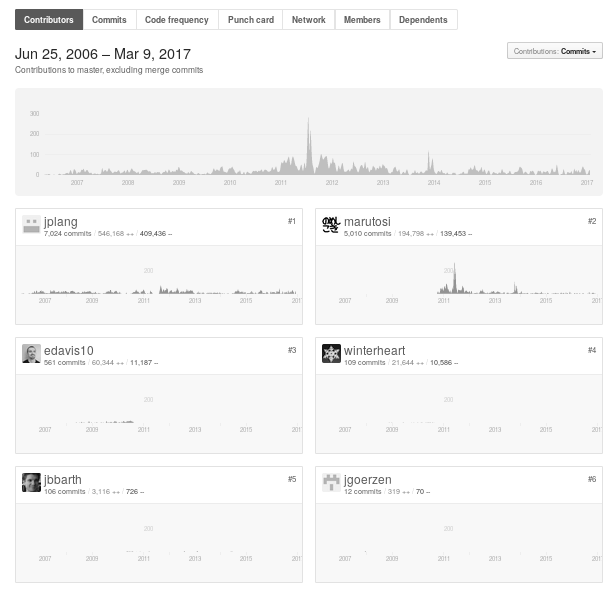
\includegraphics[width=0.8\linewidth]{./chapter-sugestoes-melhorias-fgrm/img/redmine_contribuidores.png}
	\caption{Lista de contribuidores do projeto Redmine}
\label{fig:redmine_contribuidores}
\end{figure}

\subsection{Desenho do Questionário}
\label{ssub:sug_melhoria_desenho_questionario}

A fim de coletar a opinião dos participantes foi utilizado um questionário
eletrônico. O formulário foi desenhado com a premissa de ser respondido em um
prazo curto, de preferência entre 5 e 10 minutos. Neste sentido, as perguntas
foram organizadas em dois grupos principais. As questões do primeiro grupo têm
por objetivo coletar a opinião dos profissionais sobre a relevância da
recomendação proposta e o grau de dificuldade em implementá-la. As perguntas
foram estruturadas de maneira a permitir respostas na forma de uma escala de
Likert em que o respondente deveria fornecer o seu nível de concordância para as
declarações que lhe foram apresentadas. No segundo grupo estamos interessados na
formação dos profissionais. Optamos por definir algumas das questões como não
obrigatórias por entendermos que a impossibilidade ou falta de interesse em
responder determinada pergunta não deveria impedir o participante de enviar os
dados de outras questões respondidas. A versão final do questionário pode ser
visualizado no Anexo~\ref{ch:app-form-sug-melhorias}.

\subsection{Processo de Aplicação}
\label{ssub:processo_de_aplicação}

O questionário foi encaminhado à amostra de interesse através de correio
eletrônico. O endereço foi coletado diretamente do projeto hospedado no Github.
Foi desenvolvido um \textit{script} na linguagem Python que permite coletar o
endereço de e-mail e automatizar o processo de envio. As mensagem foram
personalizadas de modo a identificar o nome do usuário e o projeto do Github
com base no template exibido a seguir. O pedido de participação foi enviado
para um total de 121 contribuidores no período de 28/04/2017 a 01/05/2017. A
mensagem enviada pode ser visualizada no
Anexo~\ref{ch:app-template-msg-avaliacao-sug-melhorias}.

% \fbox{\begin{minipage}{\textwidth}
% Dear \{\{real\_name \}\}!

% I’m conducting a research supervised by Rodolfo Resende \@-\@
% homepages.dcc.ufmg.br/~rodolfo and we want to evaluate a collection of
% recommendations to new features in Issue Tracking System. As part of them, we
% planned and executed a survey aiming at to reach a large-scale population of
% practitioners interested in to improve the features of that type of tool. Based
% on your area of interest, we kindly invite you to take part in the following
% survey:

% \{\{url\_formulario\}\}

% You were chosen because your contribution in the project \{\{nome\_grupo\}\}
% \@-\@ \{\{url\_grupo\}\} hosted on the Github platform. Your opinion is
% essential to strength our findings. Please, help us answering this survey until
% May 05th. It takes 05 minutes. As soon as we conclude the data analysis, we will
% share the results with all participants and the software engineering community.
% If you have already fulfilled this questionnaire, please ignore this email.

% Thanks in advance,
% Vagner Clementino.

% \end{minipage}}

O processo de envio consistia ainda de uma segunda mensagem de ``lembrete'' após
dois dias. Esta estratégia foi adotada com base em estudos que discutem os
resultados de que o reenvio pode ser um dos fatores que aumenta a taxa de
participação em levantamentos por questionários realizados através da
web~\cite{fan2010factors}.

\section{Resultados da Avaliação das Sugestões de Melhorias}
\label{sec:resultados_avaliacao_sug_de_melhorias}

Após o envio do formulário aos participantes obtivemos um total de 29 respostas.
Como algumas das questões do formulário não eram de preenchimento obrigatório
algumas perguntas não totalizam 29 respostas. O nível de participação foi
similar ao observado em outros estudo em Engenharia de Software que utilizam o
levantamento por questionário (survey) como método de coleta de
dados~\cite{fan2010factors}. Nas próximas seções apresentamos o perfil dos
participantes, a relevância das sugestões propostas e o grau de facilidade de
implementação das mesmas.

\subsection{Perfil dos Participantes}
\label{sub:sug_melhorias_resultados_perfil_dos_participantes}

No levantamento realizado incluímos uma questão sobre qual sistema o
desenvolvedor contribui. Esta informação é importante porque contribuidores que
trabalham com ferramentas que são consideradas mais famosas e poderosas podem
ter uma maior resistência quanto à inclusão de novas funcionalidades. A
Tabela~\ref{tab:projetos_participantesmy-label} exibe o nome dos projetos que
tiveram contribuidores que preencheram o nosso formulário. Verificamos nas
primeiras posições ferramentas tradicionais como Mantis, Trac e Debbugs. As
FGRMs que tiveram menos de duas participações foram agrupados sob o termo
``OUTROS''.

\begin{table}[htpb]
\centering
\resizebox{.3\textwidth}{!}{%
\begin{tabular}{@{}cc@{}}
\toprule
\textbf{Projeto} & \textbf{Participantes} \\ \midrule
DEBBUGS & 4 \\
MANTISBT & 4 \\
TRAC & 4 \\
FOSSIL & 3 \\
BUGZILLA & 2 \\
REDMINE & 2 \\
OUTROS & 6 \\
\bottomrule
\end{tabular}%
}
\caption{Projetos que os participantes contribuem.}
\label{tab:projetos_participantesmy-label}
\end{table}

Com relação à função desempenhada mais da metade dos participantes são
desenvolvedores (53\%). O segundo grupo de cargo com maior frequência são
aqueles ligados ao gerenciamento de equipes (Gerentes de Projetos,
\textit{Chief Technical Officer} e etc.). Verificamos ainda a participação de
Engenheiros e Arquitetos de Software. Sobre o tempo de experiência, o
percentual de 45\% dos respondentes tem entre dez e vinte anos de experiência.
A maior parte desempenha suas atividades em equipes com 2 a 5 pessoas ou com
mais do 10 membros. Quando questionamos sobre qual o tipo de atividade
desempenhada pelo participante, cerca de 85\% trabalham com desenvolvimento ou
manutenção de software. Com base no perfil apurado entendemos que os
participantes são adequados para efetuar a análise das sugestões de melhorias
desta dissertação.

\subsection{Relevância das Sugestões}
\label{sub:sug_melhorias_resultados_relevancia}

As sugestões de melhorias foram apresentadas aos participantes e eles
respondiam se achavam as sugestões pertinentes mediante uma escala do tipo
Likert. A Tabela~\ref{tab:freq_percentual_avaliacao_sug_melhorias} apresenta a
frequência e o percentual de escolha para cada sugestão de melhoria. A
Figura~\ref{fig:plot_likert_avaliacao_sug_melhorias} exibe o nível de aceitação
das sugestões propostas. Em uma primeira análise verificamos que a maioria das
recomendações tiveram uma avaliação positiva dos participantes (Concordo ou
Concordo Fortemente). A exceção foi para a Sugestão \#3 \@-\@ \textit{As FGRMs
    deveriam permitir um ranqueamento das RMs de acordo com a reputação do
    Reportador} que trata da possibilidade de ordenar as RMs a serem analisadas
pela reputação do Reportador. Por outro lado, as Sugestões \#6 \@-\@ \textit{As
    FGRMs deveriam dar suporte além da especificação de texto simples}  e \#8
\@-\@ \textit{As FGRMs deveriam suportar tarefas compartilhadas, permitindo o
    trabalho colaborativo}  tiveram uma boa aceitação dos participantes.

\begin{table}[htpb]
\centering
\resizebox{.9\textwidth}{!}{%
\begin{tabular}{@{}cccccc@{}}
\toprule
\textbf{Sugestão} & \textbf{Discordo Fortemente} & \textbf{Discordo} & \textbf{Não concordo e nem discordo} & \textbf{Concordo} & \textbf{Concordo Fortemente} \\ \midrule
\textit{Sugestão \#1} & 1 (3,4\%) & 3 (10,3\%) & 10 (34,5\%) & 13 (44,9\%) & 2 (6,9\%) \\
\textit{Sugestão \#2} & 0 (0,0\%) & 2 (6,9\%) & 7 (24,1\%) & 13 (44,9\%) & 7 (24,1\%) \\
\textit{Sugestão \#3} & 3 (10,3\%) & 9 (31,0\%) & 13 (44,9\%) & 2 (6,9\%) & 2 (6,9\%) \\
\textit{Sugestão \#4} & 0 (0,0\%) & 1 (3,4\%) & 6 (20,7\%) & 12 (41,4\%) & 10 (34,5\%) \\
\textit{Sugestão \#5} & 1 (3,4\%) & 0 (0,0\%) & 5 (17,2\%) & 10 (34,5\%) & 13 (44,9\%) \\
\textit{Sugestão \#6} & 0 (0,0\%) & 1 (3,4\%) & 2 (6,9\%) & 6 (20,7\%) & 20 (69,0\%) \\
\textit{Sugestão \#7} & 1 (3,4\%) & 5 (17,2\%) & 8 (27,7\%) & 6 (20,7\%) & 9 (31,0\%) \\
\textit{Sugestão \#8} & 0 (0,0\%) & 1 (3,4\%) & 1 (3,4\%) & 15 (51,7\%) & 12 (41,4\%) \\ \bottomrule
\end{tabular}%
}
\caption{Frequência e percentual das respostas sobre a relevância das sugestões de melhorias}
\label{tab:freq_percentual_avaliacao_sug_melhorias}
\end{table}

\begin{figure}[htpb]
    \centering
    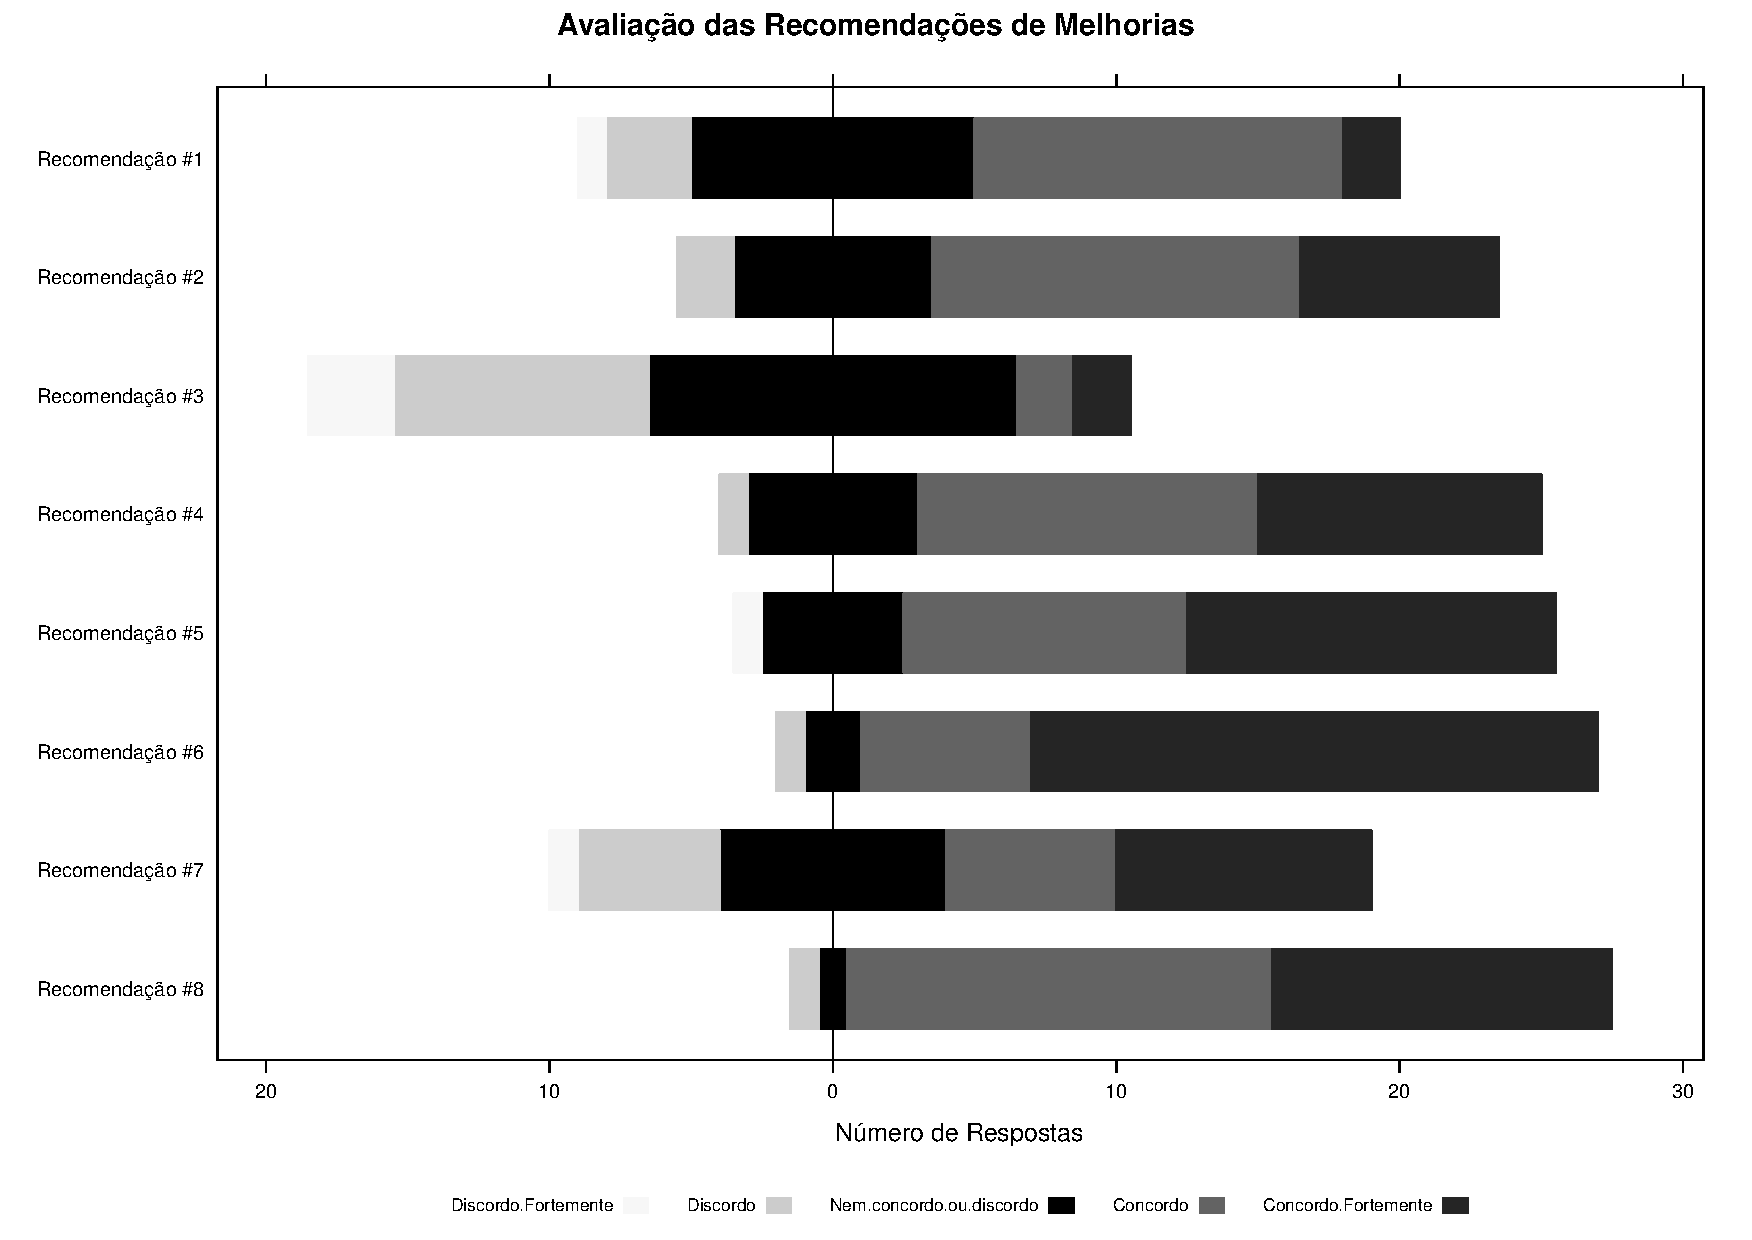
\includegraphics[width=.9\linewidth]{chapter-sugestoes-melhorias-fgrm/img/plot_likert_avaliacao_sug_melhorias_grayscale.pdf}
    \caption{Avaliação das Sugestões de Melhorias}\label{fig:plot_likert_avaliacao_sug_melhorias}
\end{figure}

Para avaliar quais sugestões tiveram maior aceitação definimos um ranqueamento.
O ordenamento consistiu em aplicar pesos para cada item da escala de Likert
conforme a Tabela~\ref{tab:pesos_rank_sug_melhorias}. O valor é obtido
multiplicando a frequência de determinado item da escala pelo seu respectivo
peso. A Tabela~\ref{fig:plot_likert_avaliacao_sug_melhorias} exibe as
recomendações ordenadas pelo nível de aceitação dos participantes, conforme o
valor atribuído a cada opção da escala Likert. É possível visualizar o número
de respostas que cada item recebeu.

\begin{table}[htpb]
\centering
\resizebox{.3\textwidth}{!}{%
\begin{tabular}{@{}lc@{}}
\toprule
\multicolumn{1}{c}{\textbf{Item da Escala}} & \textbf{Peso} \\ \midrule
Discordo Fortemente & -2 \\
Discordo & -1 \\
Nem concordo ou discordo & 0 \\
Concordo & 1 \\
Concordo Fortemente & 2 \\ \bottomrule
\end{tabular}%
}
\caption{Pesos utilizados para ordenar as sugestões propostas.}
\label{tab:pesos_rank_sug_melhorias}
\end{table}

Com base na Tabela~\ref{tab:ranking-sugestoes-melhorias} verificamos que
recomendações que sobressaíram: utilização nas FGRMs de uma linguagem além do
texto simples para redigir uma RM (\#3), suporte à tarefas colaborativas (\#8)
e incorporação de processos de Integração Contínua (\#5). Por outro lado as
sugestões de diferenciar as RMs pela reputação do Reportador (\#3) e avaliar a
qualidade do relato (\#1) não foram avaliadas como as mais relevantes pelos
participantes. É importar notar que as recomendações que ficaram nas últimas
posições tiveram a opção ``Não concordo nem discordo'' selecionadas com maior
frequência. Este fato pode indicar que não houve uma rejeição pelos
participantes, mas possivelmente, uma baixa compreensão do que estava sendo
proposto, ou ainda que não tinham opinião formada.

\begin{table}[htpb]
\centering
\resizebox{\textwidth}{!}{%
\begin{tabular}{@{}lcccccc@{}}
\toprule
\multicolumn{1}{c}{\textbf{Sugestão}} & \textbf{Discordo Fortemente} &
\textbf{Discordo} & \textbf{Não concordo e nem discordo} & \textbf{Concordo} &
\textbf{Concordo Fortemente} & \textbf{Ranking} \\ \midrule
\textit{Sugestão \#6} & 0 & 1 & 2 & 6 & 20 & 45 \\
\textit{Sugestão \#8} & 0 & 1 & 1 & 15 & 12 & 38 \\
\textit{Sugestão \#5} & 1 & 0 & 5 & 10 & 13 & 34 \\
\textit{Sugestão \#4} & 0 & 1 & 6 & 12 & 10 & 31 \\
\textit{Sugestão \#2} & 0 & 2 & 7 & 13 & 7 & 25 \\
\textit{Sugestão \#7} & 1 & 5 & 8 & 6 & 9 & 17 \\
\textit{Sugestão \#1} & 1 & 3 & 10 & 13 & 2 & 12 \\
\textit{Sugestão \#3} & 3 & 9 & 13 & 2 & 2 & -9 \\ \bottomrule
\end{tabular}%
}
\caption{Ranking das sugestões propostas}
\label{tab:ranking-sugestoes-melhorias}
\end{table}

\subsection{Implementação das Sugestões}
\label{sub:sug_melhorias_resultados_implementacao}

Neste etapa do estudo estávamos interessados em avaliar o nível de dificuldade
para implementar as sugestões propostas. A frequência e o percentual das
respostas para cada sugestão de melhoria estão disponíveis na
Tabela~\ref{tab:freq_percent_aval_sug_melhorias_implementacao} e podem ser
visualizados na Figura~\ref{fig:plot_likert_avaliacao_implementacao_melhorias}

\begin{table}[htpb]
\centering
\resizebox{\textwidth}{!}{%
\begin{tabular}{@{}cccccc@{}}
\toprule
\textbf{Sugestão} & \textbf{Discordo Fortemente} & \textbf{Discordo} & \textbf{Não concordo e nem discordo} & \textbf{Concordo} & \textbf{Concordo Fortemente} \\ \midrule
\textit{Sugestão \#1} & 1 (3,4\%) & 3 (10,3\%) & 10 (34,5\%) & 13 (44,9\%) & 2 (6,9\%) \\
\textit{Sugestão \#2} & 0 (0,0\%) & 2 (6,9\%) & 7 (24,1\%) & 13 (44,9\%) & 7 (24,1\%) \\
\textit{Sugestão \#3} & 3 (10,3\%) & 9 (31,0\%) & 13 (44,9\%) & 2 (6,9\%) & 2 (6,9\%) \\
\textit{Sugestão \#4} & 0 (0,0\%) & 1 (3,4\%) & 6 (20,7\%) & 12 (41,4\%) & 10 (34,5\%) \\
\textit{Sugestão \#5} & 1 (3,4\%) & 0 (0,0\%) & 5 (17,2\%) & 10 (34,5\%) & 13 (44,9\%) \\
\textit{Sugestão \#6} & 0 (0,0\%) & 1 (3,4\%) & 2 (6,9\%) & 6 (20,7\%) & 20 (69,0\%) \\
\textit{Sugestão \#7} & 1 (3,4\%) & 5 (17,2\%) & 8 (27,7\%) & 6 (20,7\%) & 9 (31,0\%) \\
\textit{Sugestão \#8} & 0 (0,0\%) & 1 (3,4\%) & 1 (3,4\%) & 15 (51,8\%) & 12 (41,4\%) \\ \bottomrule
\end{tabular}%
} \caption{Frequência e percentual das respostas sobre a dificuldade de
    implementação das
    sugestões de melhoria}\label{tab:freq_percent_aval_sug_melhorias_implementacao} \end{table}

\begin{figure}[htpb]
    \centering
    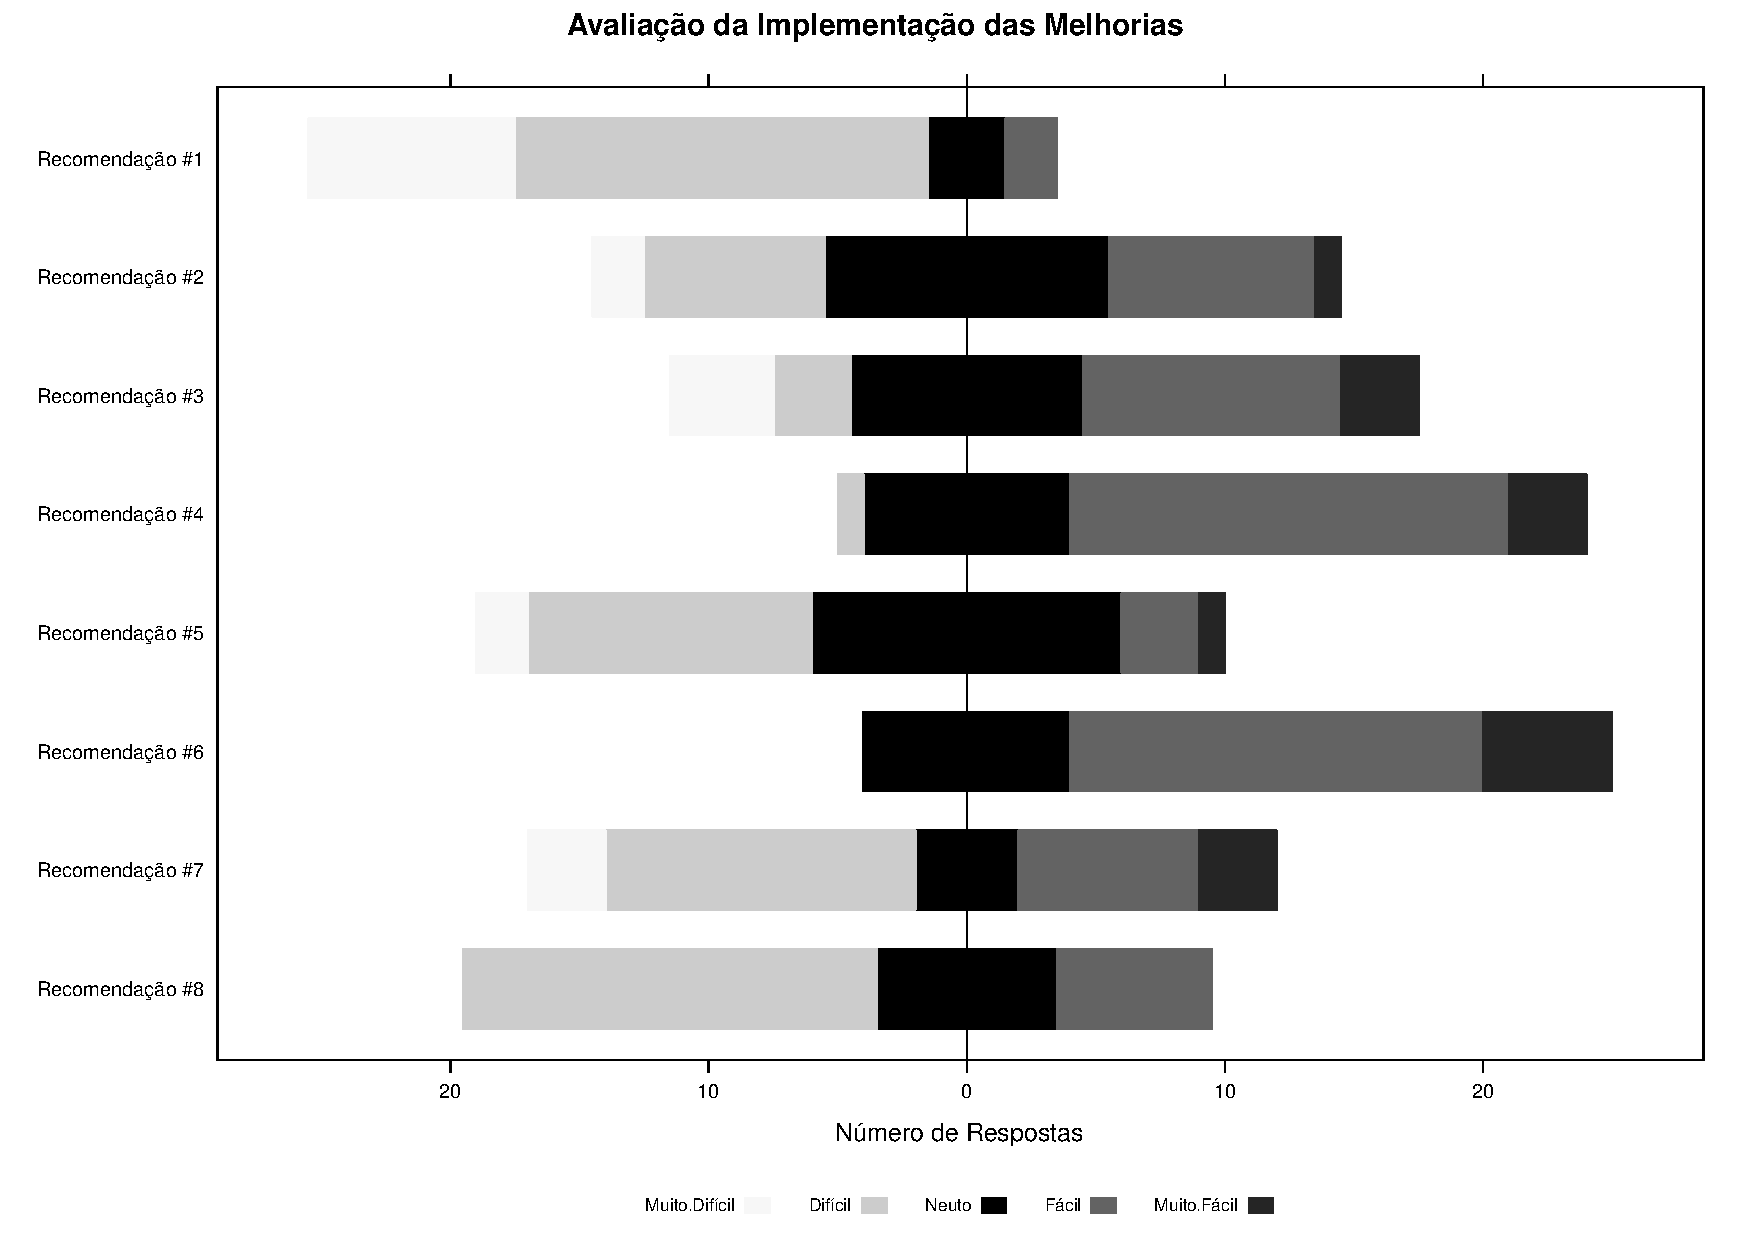
\includegraphics[width=1.1\linewidth]{chapter-sugestoes-melhorias-fgrm/img/plot_likert_avaliacao_implementacao_melhorias_grayscale.pdf}
    \caption{Avaliação sobre a  implementação das sugestões propostas.}
\label{fig:plot_likert_avaliacao_implementacao_melhorias}
\end{figure}

As sugestões foram ordenadas pelo grau de dificuldade de implementação.
Utilizamos um mecanismo similar ao descrito na
Seção~\ref{sub:sug_melhorias_resultados_relevancia} em que o valor é obtido
multiplicando a frequência de um item da escala por valor previamente definido,
que chamamos de peso. Os pesos estão apresentados na
Tabela~\ref{tab:pesos-implementacao-sug-melhorias}.

\begin{table}[htpb]
\centering
\resizebox{.2\textwidth}{!}{%
\begin{tabular}{@{}ll@{}}
\toprule
Item da Escala & Peso \\ \midrule
Muito Difícil & -2 \\
Difícil & -1 \\
Neutro & 0 \\
Fácil & 1 \\
Muito Fácil & 2 \\ \bottomrule
\end{tabular}%
}
\caption{Pesos utilizados no ranqueamento das sugestões de melhorias}
\label{tab:pesos-implementacao-sug-melhorias}
\end{table}

Foram consideradas ser de fácil implementação: o suporte do relato de uma RM
além do texto simples (\#6), a criação de atalhos e filtros personalizáveis
(\#4) e o ranqueamento das RMs pela reputação do Reportador (\#3). Segundo os
participantes funções como o suporte a tarefas compartilhadas (\#8) e análise
da qualidade do relato (\#1) foram consideradas de um maior grau de dificuldade
de implementação. O fato interessante é que a Sugestão \#3 foi considerada como
uma das mais fáceis de implementar, entretanto, está entre aquelas que tiveram
menor aceite entre os participantes. Este fato pode sugerir que sua possível
rejeição não estaria ligada à sua complexidade de desenvolvimento, mas a
fatores como não haver interesse em classificar aqueles que reportam uma RM\@.
Em geral, ao analisarmos a
Figura~\ref{fig:plot_likert_avaliacao_implementacao_melhorias} é possível
verificar que os participantes entenderam que metade das sugestões propostas
possuem uma dificuldade que pode ser considerada mediana. Contudo, as sugestões
\#1, \#5 e \#8 parecem ter sido consideradas difíceis.

\begin{table}[htpb]
\centering
\resizebox{\textwidth}{!}{%
\begin{tabular}{@{}ccccccc@{}}
\toprule
\multicolumn{1}{l}{\textbf{Recomendações}} & \multicolumn{1}{l}{\textbf{Muito
        Difícil}} & \multicolumn{1}{l}{\textbf{Difícil}} &
\multicolumn{1}{l}{\textbf{Neutro}} & \multicolumn{1}{l}{\textbf{Fácil}} &
\multicolumn{1}{l}{\textbf{Muito Fácil}} & \multicolumn{1}{l}{\textbf{Ranking}}
\\ \midrule
Sugestão \#6 & 0 & 0 & 8 & 16 & 5 & 26 \\
Sugestão \#4 & 0 & 1 & 8 & 17 & 3 & 22 \\
Sugestão \#3 & 4 & 3 & 9 & 10 & 3 & 5 \\
Sugestão \#2 & 2 & 7 & 11 & 8 & 1 & -1 \\
Sugestão \#7 & 3 & 12 & 4 & 7 & 3 & -5 \\
Sugestão \#5 & 2 & 11 & 12 & 3 & 1 & -10 \\
Sugestão \#8 & 0 & 16 & 7 & 6 & 0 & -10 \\
Sugestão \#1 & 8 & 16 & 3 & 2 & 0 & -30 \\
\bottomrule
\end{tabular}%
}
\caption{Ordenamento das sugestões pelo grau de dificuldade.}
\label{tab:ranking_implementacao_sug_melhorias}
\end{table}

\section{Discussão}
\label{sec:sug_melhoria_discussao}

Em geral podemos considerar que as sugestões propostas tiveram uma boa
aceitação dos participantes. Em média 32\% dos participantes avaliaram as
recomendações ``Concordo'' ou ``Concordo Fortemente''.  Além disso, por volta
de 22\% em média selecionaram a opção ``Nem concordo ou discordo''. Uma questão
a ser futuramente investigada é se as as respostas poderiam ser alteradas para
uma visão mais positiva, com por exemplo ``Concordo'' ou ``Concordo
Fortemente'', caso fossem fornecidos mais detalhes ao participantes. Com este
objetivo um estudo do tipo entrevista poderia ser conduzido.

Com relação às recomendações propostas, verificamos que a utilização de uma
linguagem além do texto simples, como por exemplo o Markdown, foi muito bem
aceita. Este tipo de sugestão tem como principal objetivo aumentar o poder
de expressão do relato, tal como a possibilidade do destaque da sintaxe do
código fonte. Conforme pode ser observado na
Seção~\ref{sec:caracterizacao_ferramentas} trata-se de uma funcionalidade
encontrada em uma das FGRMs analisadas. Entretanto, o nosso resultado demonstra,
com base na amostra utilizada, que deveria ser estendida para outras
ferramentas.

O suporte a tarefas compartilhadas (sugestão \#8) também foi muito bem aceita.
Esta recomendação surgiu das tentativas de implantação das propostas dos
agilistas~\cite{svensson2005introducing}. A sugestão defende que uma
determinada RM não tenha um único ``dono'', mas que a responsabilidade seja
dividida entre dois ou mais membros da equipe. Esta divisão de tarefas pode
resultar na melhor distribuição do conhecimento entre a equipe. A prevalência
deste tipo de funcionalidade pode estar relacionada com o desejo das equipes de
manutenção de utilizar algumas das práticas dos agilistas. Seria necessário um
aprofundamento da opinião dos participantes para confirmamos esta hipótese.
Apesar da sua popularidade entre os participantes, esta sugestão ficou entre
aquelas com maior grau de dificuldade de implementação.

Por outro lado, as sugestões que têm algum tipo de relação com a interface das
FGRMs (sugestões \#6, \#4, e \#2) foram consideradas como mais ``fácil'' de
implementar com mais frequência. Entretanto, a sugestão sobre a qualidade do
relato (\#1) ficou entre aquelas com maior grau de dificuldade. Esta
classificação pode ser decorrente do caráter subjetivo que a qualidade do
relato pode ter. Em cada projeto a qualidade do relato pode ter características
distintas o que pode dificultar o seu suporte.

\section{Ameaças à Validade}
\label{sec:sug_melhoria_ameacas}

Para avaliarmos as sugestões propostas utilizamos um levantamento empregando
uma amostra de conveniência. Apesar da taxa de resposta estar dentro da faixa
observada na literatura, o total de participantes não nos permite extrapolar os
resultados para todos os contextos em que as FGRMs estão inseridas.
Adicionalmente, os critérios utilizados para seleção, como por exemplo, seis
meses de desenvolvimento ou ter no mínimo duzentas revisões, não nos permite
afirmar que foram escolhidos os projetos mais representativos para o nosso
público-alvo. A utilização de apenas projetos públicos hospedados no Github
pode ter causado algum tipo de direcionamento, como por exemplo foco em
projetos de código aberto.

A estrutura das perguntas do formulário pode ter causado impacto na quantidade
de respostas ou na opção escolhida pelos participantes. Esta situação pode ter
ocorrido especialmente quando apresentamos as sugestões. No caso de escrevermos
de maneira extensa a explicação corremos o risco do respondente desistir do
item. Entretanto, se o texto fosse escrito de forma ``concisa'' corremos o
risco de ficar vago, o que pode ter impacto nas respostas. O ideal seria uma
descrição concisa associada com uma explicação detalhada. A opção por apenas
uma descrição concisa pode fazer com que a pesquisa ficasse superficial. A
Tabela~\ref{tab:projetos_participantesmy-label} detalha os projetos que os
participantes contribuem. É possível observar que os participantes trabalham
com ferramentas que são mais famosas e portanto têm o viés de visão mais
``tradicional''.

Em um dos comentários um dos participantes citou que algumas das sugestões
propostas podem ter funcionalidades similares em outras FGRMs. Acreditávamos
que a escolha destas 08 sugestões envolveria as principais melhorias para as
funcionalidades das FGRMs, mas existia a possibilidade de alguma sugestão
existir de forma parcial ou completa em determinada ferramenta. A condução da
avaliação das sugestões melhorias foi realizada também para identificar este
tipo de situação.

\section{Resumo do Capítulo}\label{sec:sug_melhoria_resumo}

O objetivo do levantamento foi avaliar as sugestões de melhorias de
funcionalidades das FGRMs. A avaliação foi realizada com base na opinião de
desenvolvedores que contribuem para projetos de código aberto deste tipo de
software. Em geral, as sugestões de melhorias foram bem avaliadas. Das 8
sugestões propostas 5 foram avaliadas de forma positiva (``Concordo'' ou
``Concordo Fortemente''). Quanto à dificuldade de implementação, metade delas
foi considerada de fácil implementação. No próximo capítulo discutimos aspectos
de implementação da Sugestão \#1 na plataforma Github.


%Incluindo o fonte do Capítulo 07
%\chapter{Avaliação das Extensões para Ferramentas de Gerenciamento de Requisição de Mudança}

\section{Introdução}

\section{Resumo do Capítulo}


%Incluindo o fonte do Capítulo 07
\chapter{Conclusão}
\label{ch:conclusao_trab_futuros}

A Manutenção de Software é um processo complexo e caro e, portanto, merece
atenção da comunidade científica e da indústria. Neste contexto, surge a
necessidade do desenvolvimento de técnicas, processos e ferramentas que reduzam
o custo e o esforço envolvidos nas atividades de manutenção e evolução de
software. Neste contexto, as Ferramentas de Gerenciamento de Requisição de
Mudança desempenham um papel fundamental que ultrapassa a simples função de
registrar as falhas e os pedidos de melhoria dos softwares. Este estudo se
propôs a avaliar as funcionalidades das FGRMs de modo a melhorá-las.

Com base no estudo descrito na Seção~\ref{sec:caracterizacao_ferramentas}
verificamos que as FGRM dispõem de funcionalidades para gerenciar a criação,
consulta, atualização e destruição de uma RM\@. Entretanto, em algumas
plataformas, tais como o Github e o Gitlab, não há clara separação entre o
gerenciamento das RMs e o controle de versão de código. Uma possível
desdobramento desta dissertação é avaliar o impacto desta abordagem na
Manutenção de Software. Este tipo de análise poderia modificar o desenvolvimento
de futuras versões deste tipo de software.

No Capítulo~\ref{ch:mapeamento-sistematico}, ao revisarmos a literatura sobre
melhorias nas FGRMs, recuperamos estudos que discutem diversos aspectos dos
problemas e desafios do gerenciamento das RMs. Apesar do foco em temas como
atribuição automática e RMs duplicadas, outros estudos discutem que alguns
desenvolvedores estariam mais interessados em propostas que melhorem a qualidade
do relato da RM\@. Este é um exemplo do desacoplamento entre as necessidades dos
desenvolvedores e o que está sendo proposto na literatura. Verificamos que a
literatura da área tem se dedicado a melhoria das funções das FGRMs, contudo,
tais avanços ainda não chegaram aos desenvolvedores. Apesar deles se mostrarem
satisfeitos com as funcionalidades oferecidas, ainda existem muito outras que
poderiam se acopladas a este tipo de software de modo a melhorar as atividades
de manter e evoluir um software. Transversalmente as metodologias propostas
pelos agilistas vêm sendo adotadas por algumas equipes de manutenção de
software. Neste contexto, as FGRM podem implantar funcionalidade de modo a
suportar algumas destas práticas.

De maneira relacionada, em uma das classificações feitas no Mapeamento
conduzido, os estudos foram agrupados pelo tipo de papel desempenhado na
Manutenção de Software o qual daria suporte. Utilizamos uma classificação
proposta por Polo e outros~\cite{Polo1999} construída em 1999. Em nossas
pesquisas não identificamos uma discussão mais recente sobre os papéis
desempenhados na Manutenção de Software. Entendemos que seria importante a
realização de um novo trabalho com o objetivo de descreve e avaliar os papéis
desempenhados no processo de manter um software. Este estudo poderia avaliar
como as práticas propostas pelos agilistas podem ter alterado esta estrutura de
trabalho.

O nível de satisfação com as funcionalidades das FGRMs dos profissionais
envolvidos com Manutenção de Software pode ser considerado como alto. Esta
percepção foi obtida mediante um levantamento por questionário apresentado no
Capítulo~\ref{ch:pesquisa-profissionais}. Entretanto, o mesmo estudo demonstrou
que os participantes desconhecem o potencial deste tipo de software. No
questionário, ao apresentarmos propostas de melhorias que eram discutidas na
literatura o grau de aceitação foi bastante elevado. Neste sentido, observamos
um distanciamento entre o estado da arte e o estado da prática das melhorias das
FGRMs. Apesar deste distanciamento ser algo esperado, por diversas razões,
estudos devem ser conduzidos afim de diminuir estas diferenças. Entendemos que
esta dissertação contribuiu neste sentido ao apresentar para os profissionais
algumas das melhorias discutidas na literatura. Este conhecimento pode ser
utilizado pelos desenvolvedores para exigir ferramentas que atendam às suas
demandas. Ao mesmo tempo o nosso trabalho conseguiu coletar, discutir e
apresentar algumas da necessidades dos desenvolvedores. Da mesma forma,
pesquisadores podem usar esta informação para propor trabalhos com o intuito de
propor melhorias para as FGRMs.

Esta dissertação contribuiu para o estudo das FGRMs com a apresentação de um
conjunto de melhorias no Capítulo~\ref{ch:sug_melhoria}. Considerando a sua boa
aceitação, estas recomendações podem ser utilizadas por pesquisadores, pelos
responsáveis por desenvolver e manter projetos de FGRMs e por os profissionais
envolvidos com Manutenção de Software. Um possível desdobramento desta
dissertação é a avaliação do impacto da implantação destas sugestões. Esta
análise poderia ser realizada mediante um Estudo de Caso, por exemplo.

No Capítulo~\ref{ch:implemtacao_extensao} implementamos uma das sugestões como
uma extensão para o módulo de \textit{issues} da plataforma Github. Por ser
tratar de uma Prova de Conceito, não foi realizada uma avaliação com membros dos
projetos selecionados. Por esta razão não é possível extrapolar os resultados.
Gostaríamos de futuramente conduzir um trabalho em uma configuração em que seja
possível avaliar a opinião de alguém envolvido no projeto estudado.  A
contribuição deste trabalho de dissertação está na proposição de melhorias para
as FGRMs tomando como base a literatura em Manutenção de Software e a opinião de
profissionais envolvidos em Manutenção de Software.

% O gerenciamento das RMs formam as funcionalidades centrais de uma FGRM\@.
% Estas funções podem ser agrupadas em um termo único denominado
% \textit{Operações de
% CRUD} (acrônimo de Create, Read, Update e Delete na língua Inglesa). As
% principais categorias de funcionalidades que foram encontradas para a dimensão
% de \textit{Gestão da RM} estão descritas a seguir.

% Realmente utilizar a justificativa esforço necessário é fazer como você mesmo
% disse aumenta superfície de ataque. Acho que o ideal é colocar que no momento de
% decisão qual ferramenta analisar optamos por um número menor, não pelo esforço,
% mas por entendermos que as escolhidas poderiam caracterizar o conjunto de
% ferramentas disponíveis. Posteriormente, verificamos que a escolha não se
% mostrou ideal já que no survey induziu a alguns erros na proposição das
% melhorias.


% Incluindo bibliografia:
\ppgccbibliography{../bib/bibliografia}

% apêndices, se bhouver
\begin{appendices}

\chapter{Lista de Ferramenta de Gerenciamento de Requisição de mudanças}
\label{ch:app-lista-fgrm}
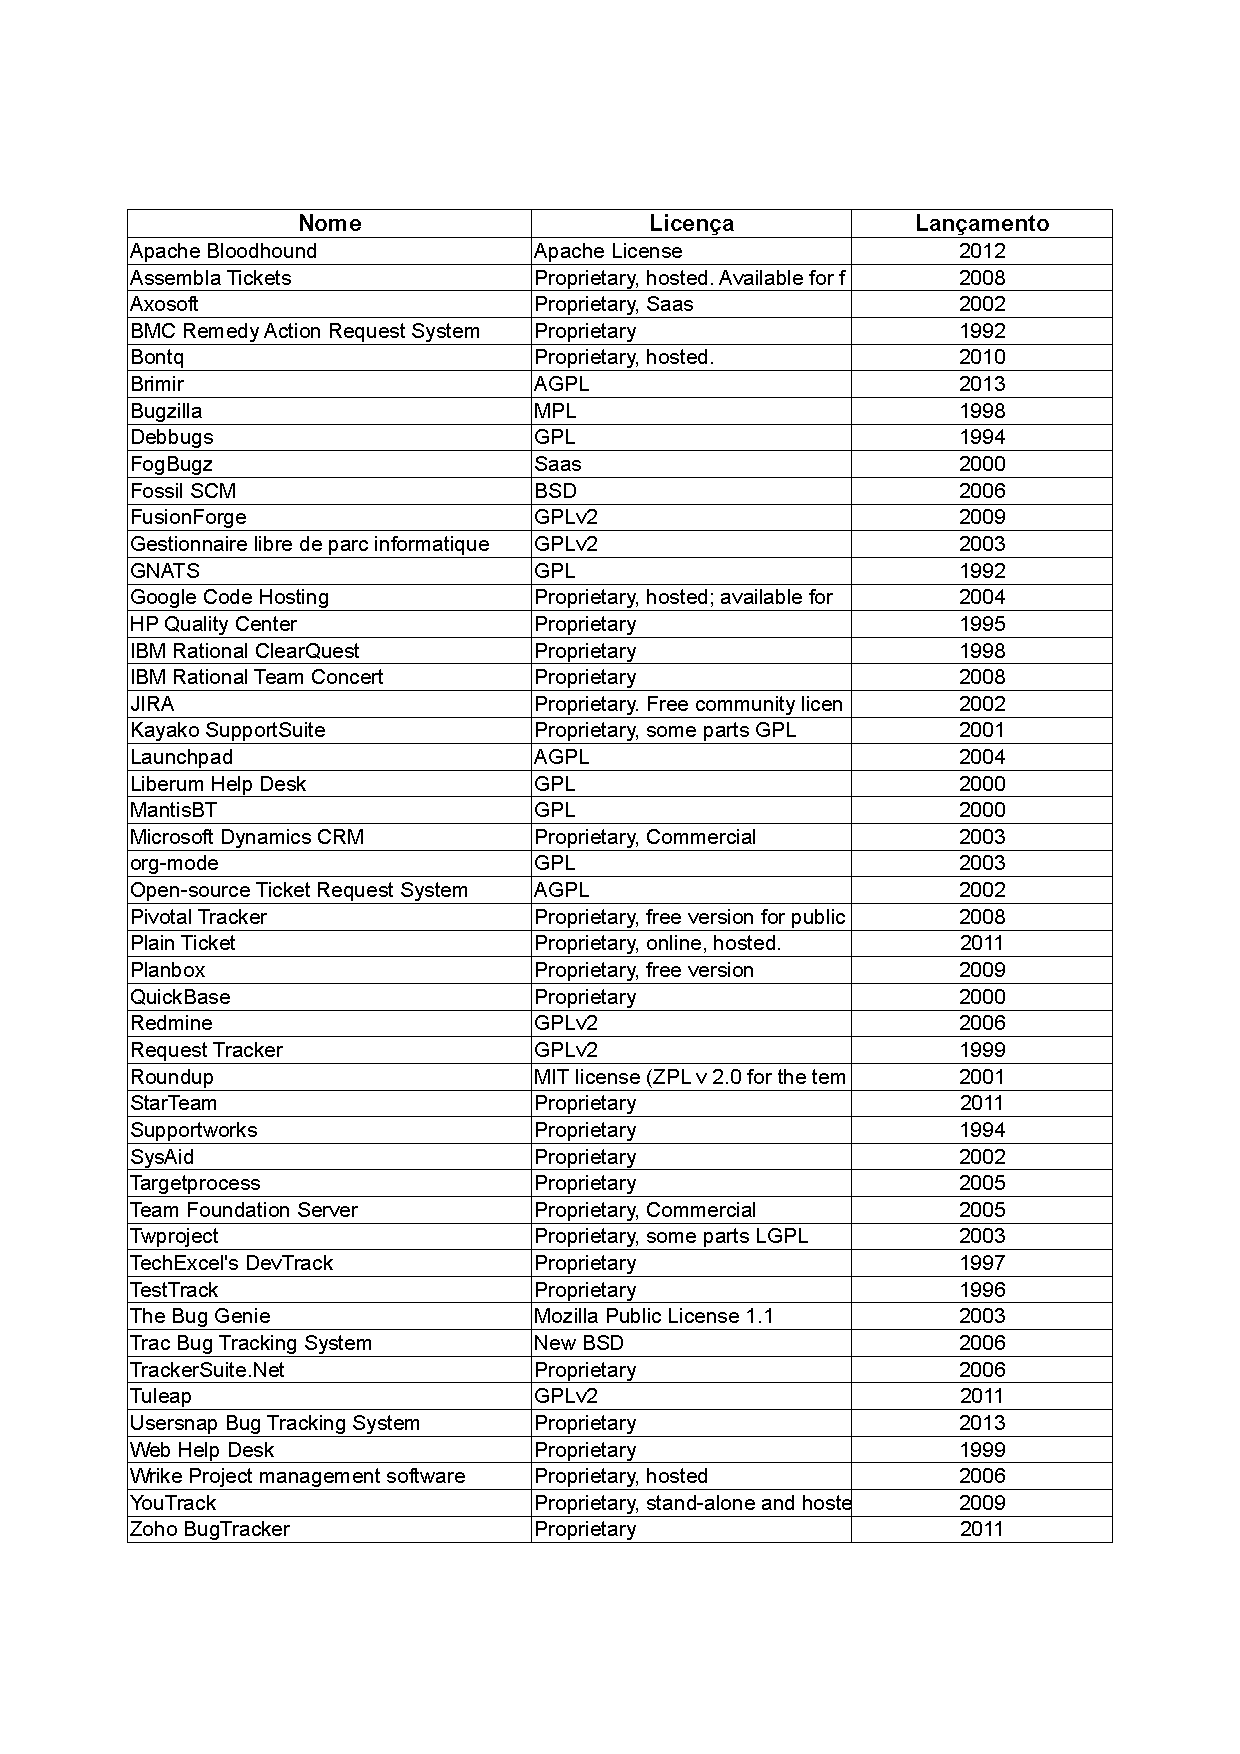
\includepdf[pages=-,scale=.8,linktodoc=true]{./apendices/img/Lista_ITS_Wikipedia.pdf}

\chapter{Formulário Aplicado para Seleção de Ferramentas}
\label{ch:app-form-selecao-ferramentas}
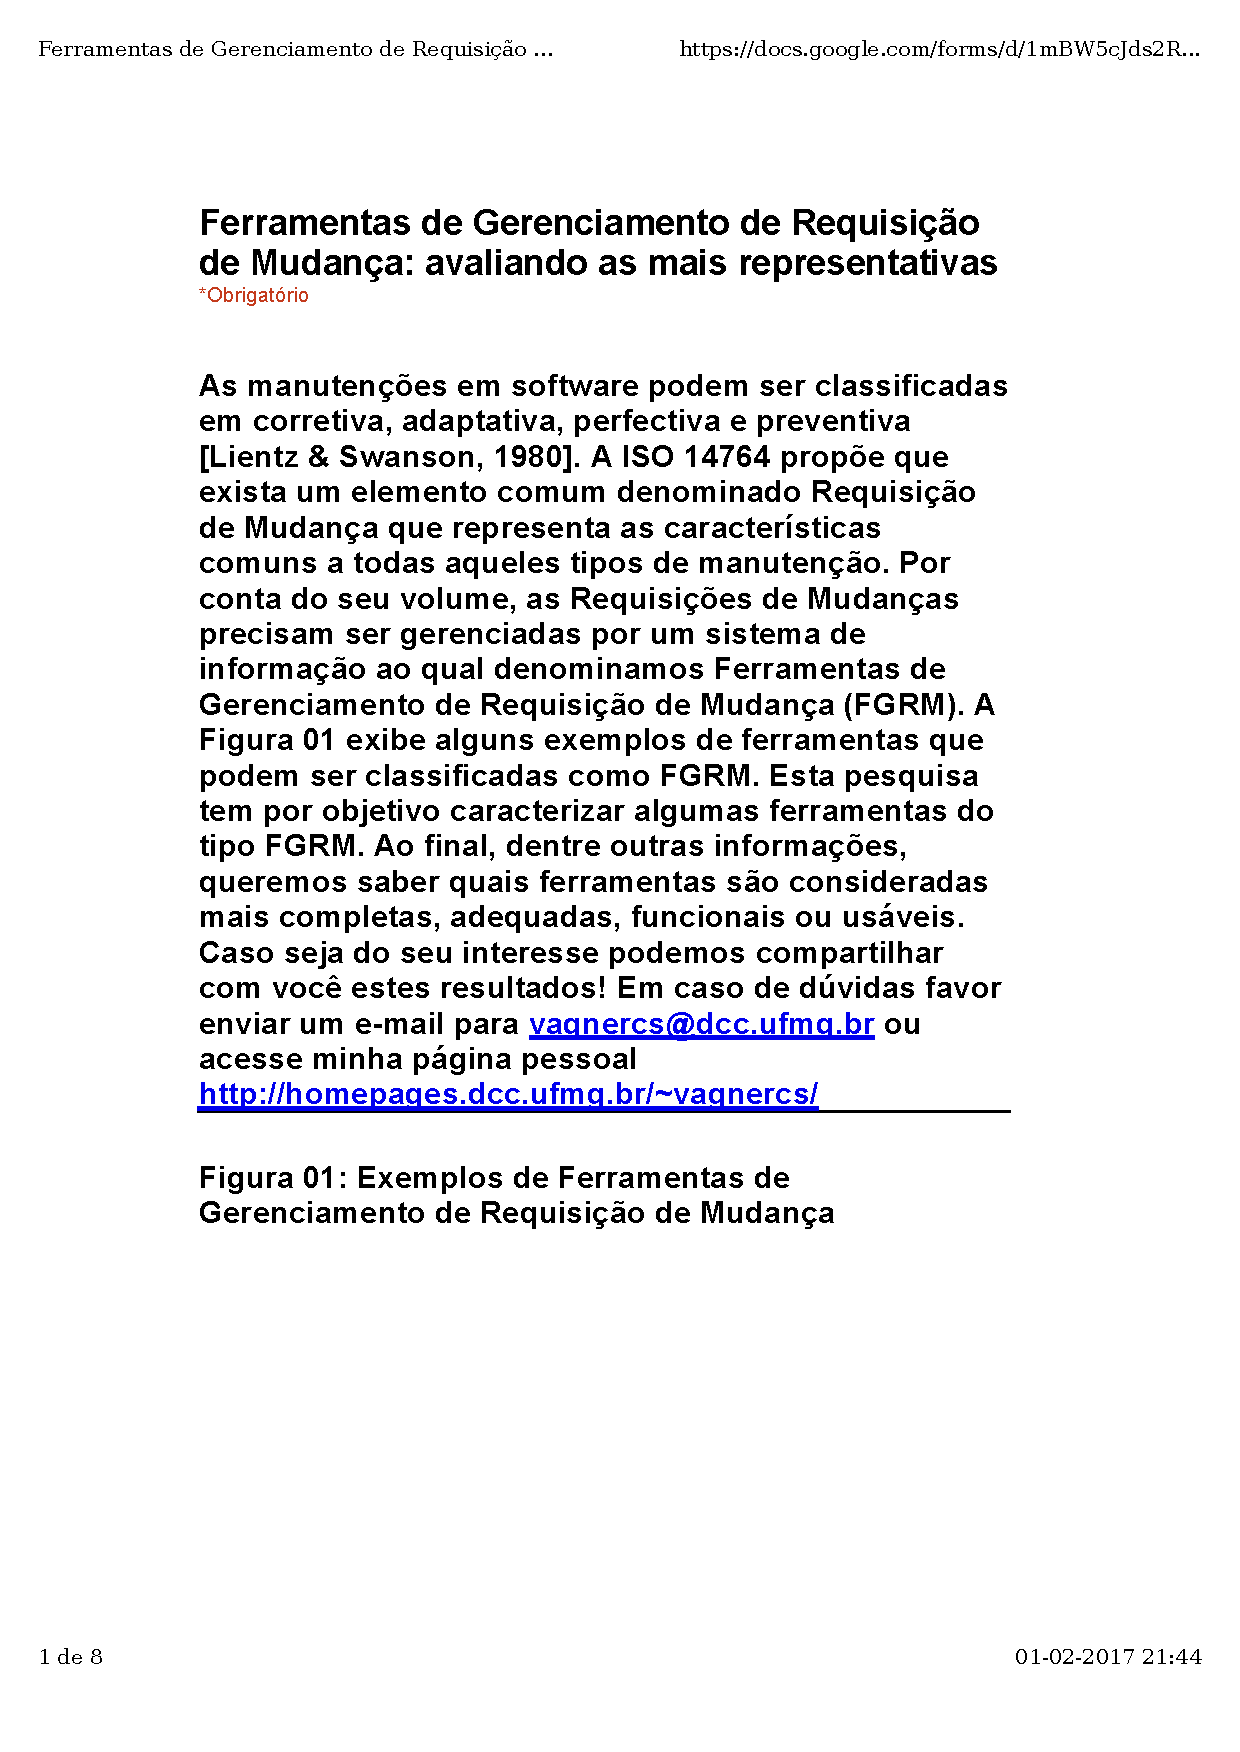
\includepdf[pages=-,scale=.8,linktodoc=true]{./apendices/img/form-avalicao-ferramentas-pt-br.pdf}

\chapter{Formulário dos Cartões Ordenados}
\label{ch:app-form-cartoes-ordenados}
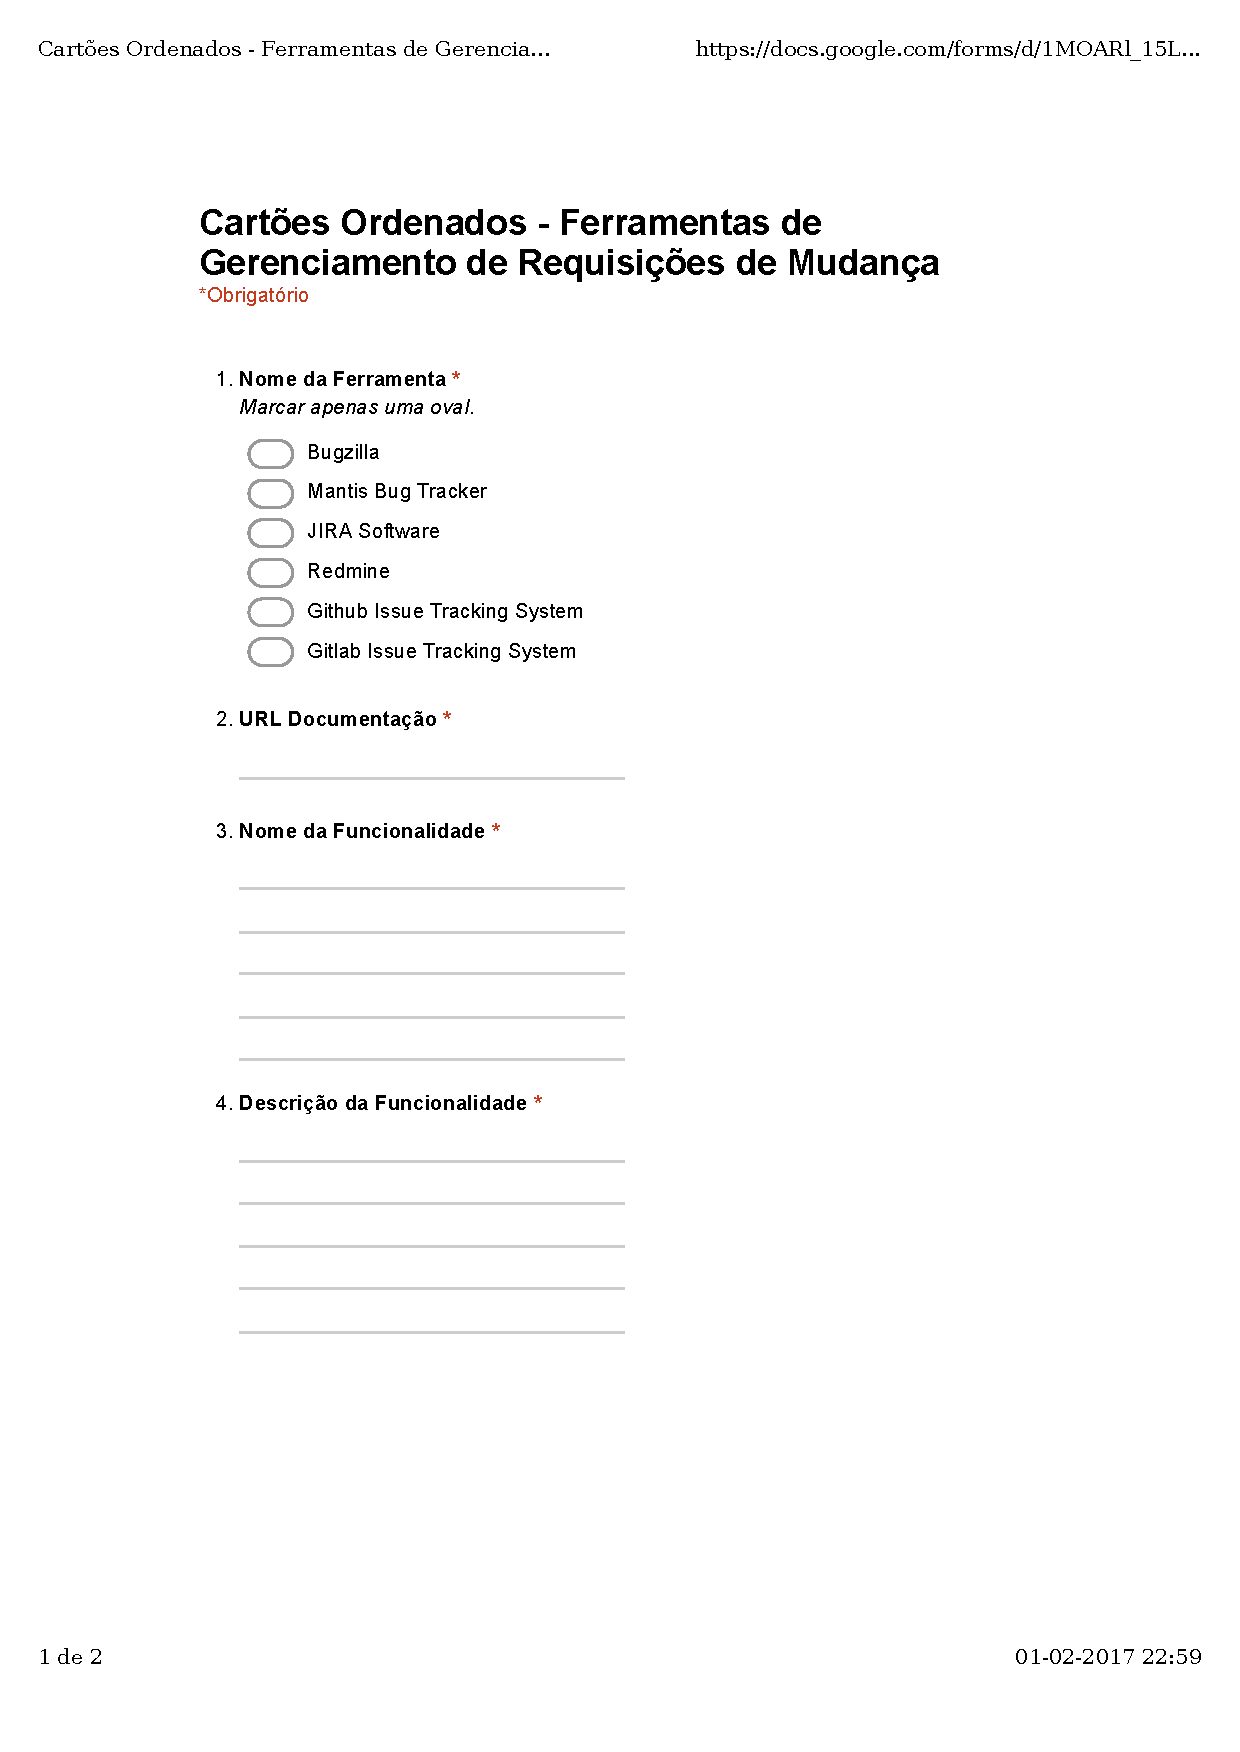
\includepdf[pages=-,scale=.8,linktodoc=true]{./apendices/img/form-cartoes-ordenados.pdf}

\chapter{Sentenças de Busca por Base de Dados}
\label{ch:app-setenca-de-busca-base-dados}
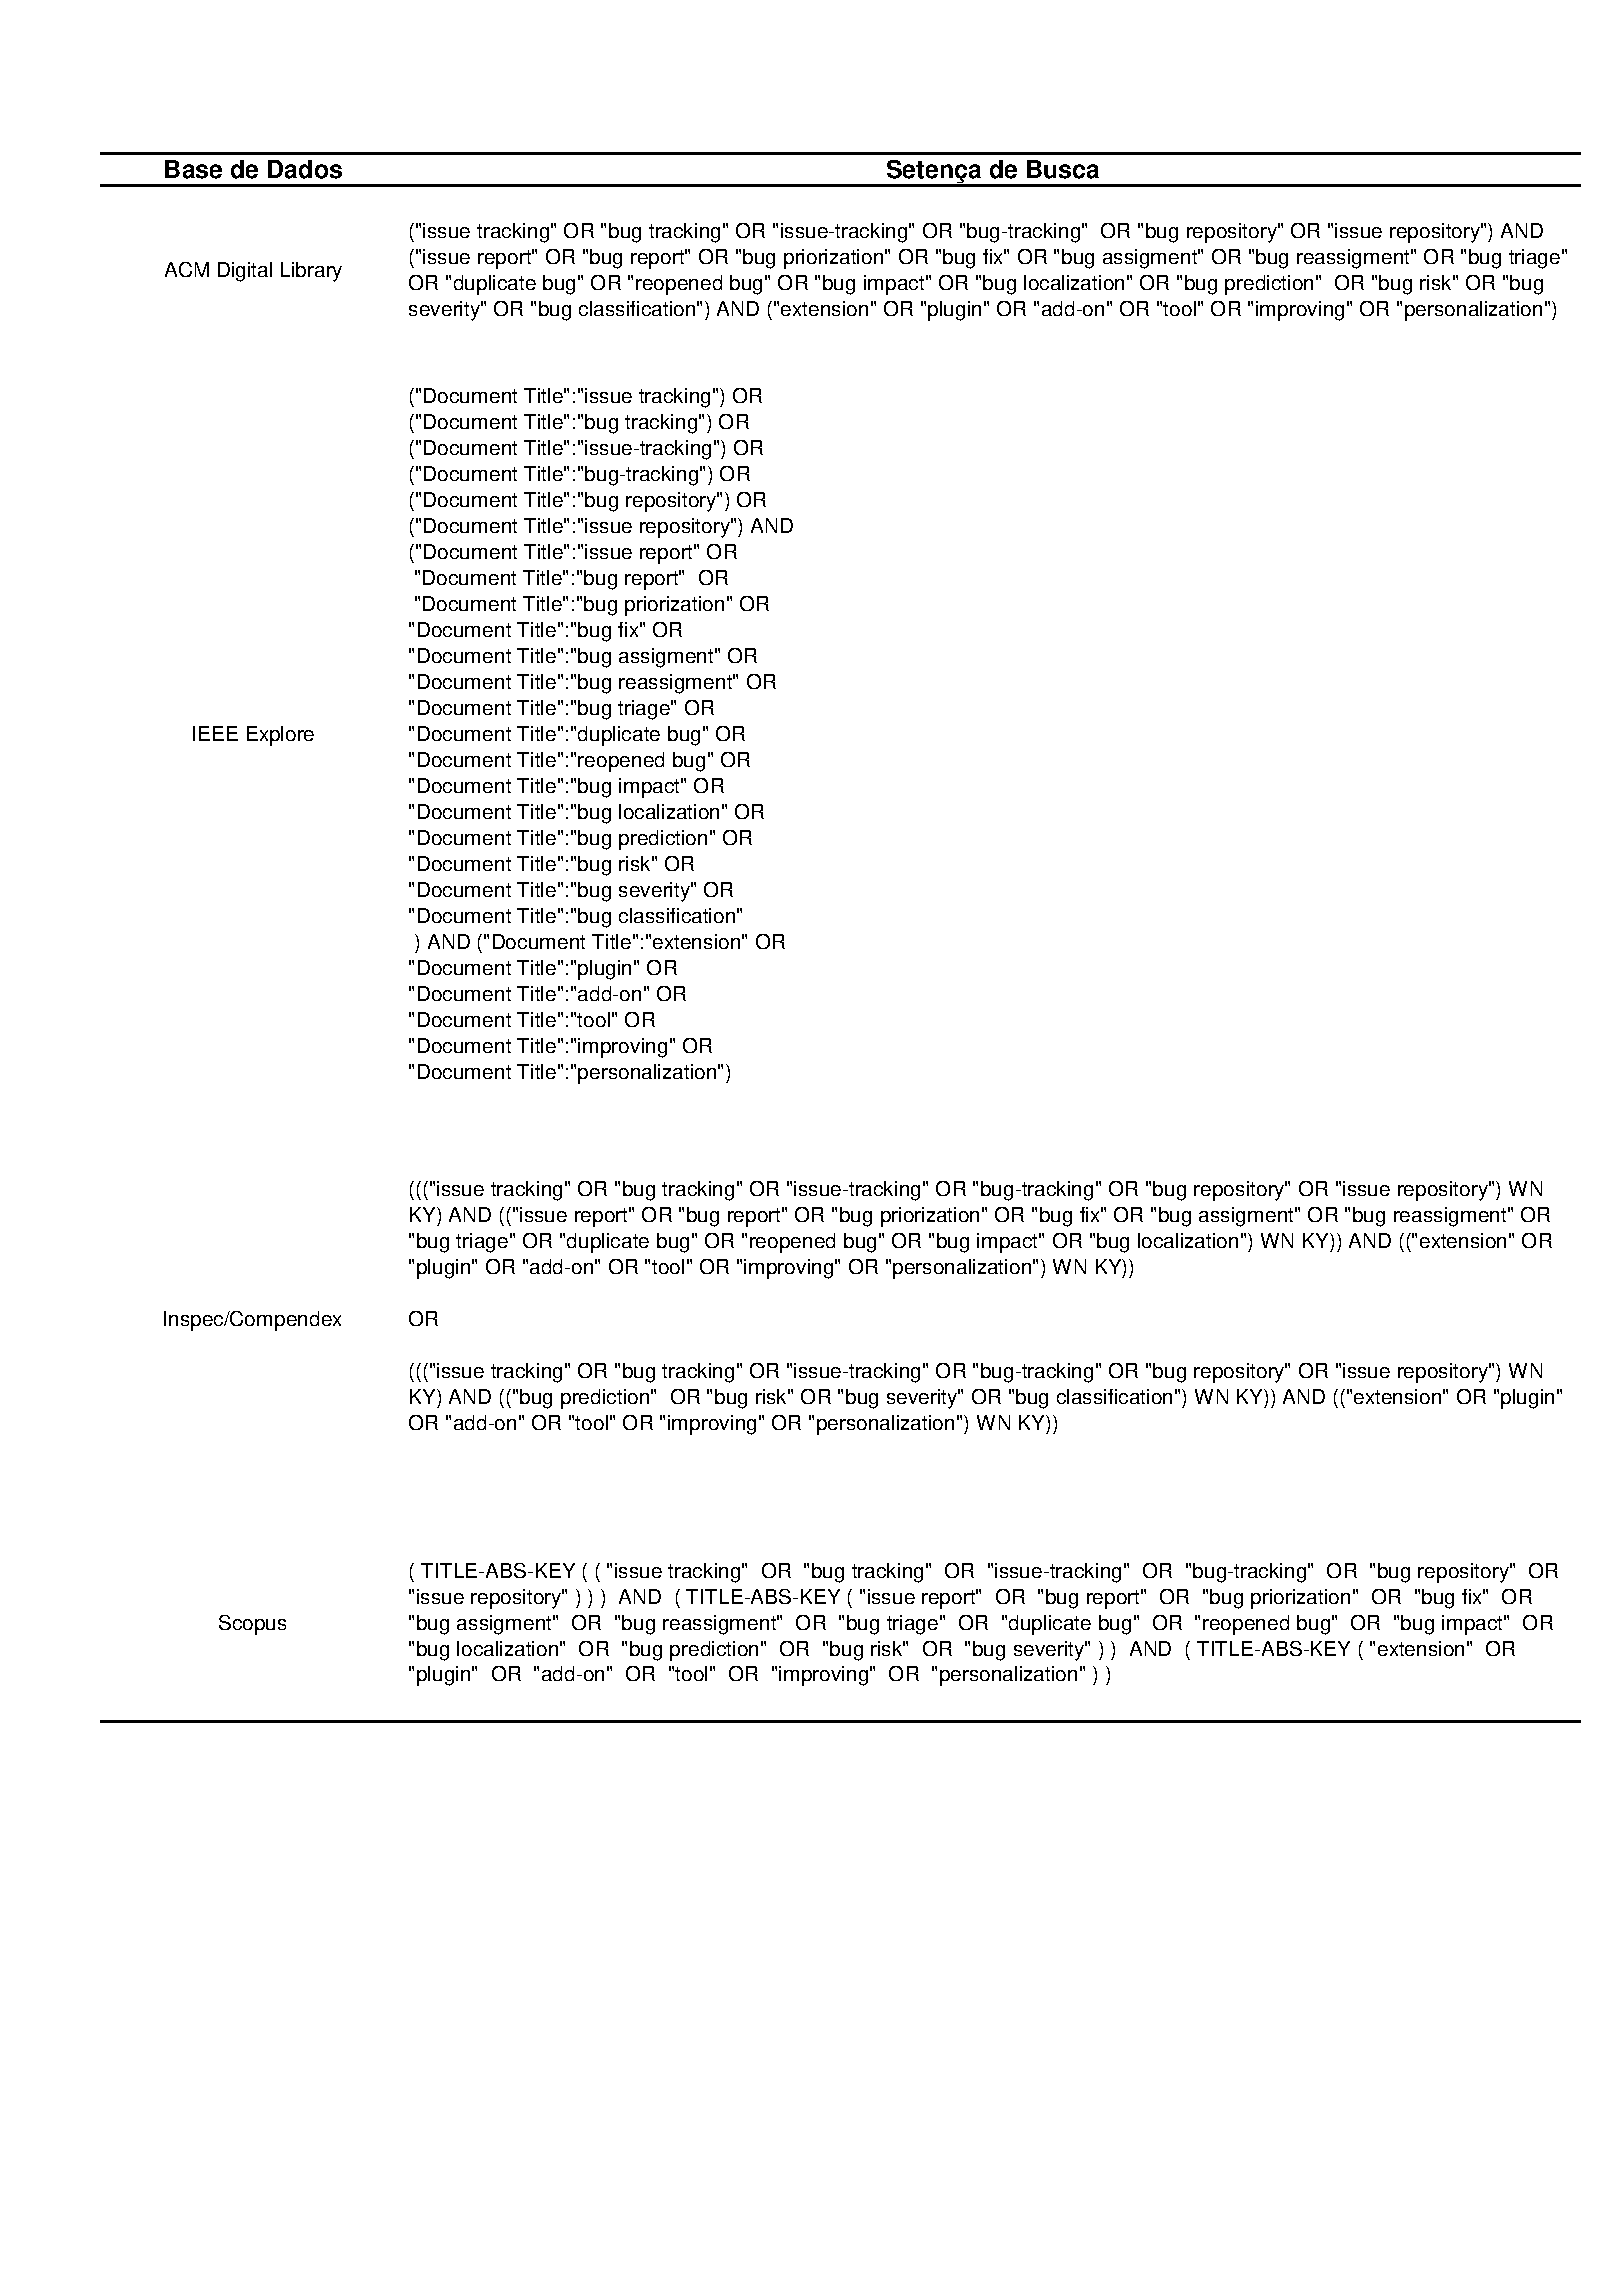
\includepdf[pages=-,scale=.8,linktodoc=true]{./apendices/img/setenca-de-busca-por-base-dados.pdf}

\chapter{Formulário Aplicado na Pesquisa com Profissionais}
\label{ch:app-form-pesq-profissionais}
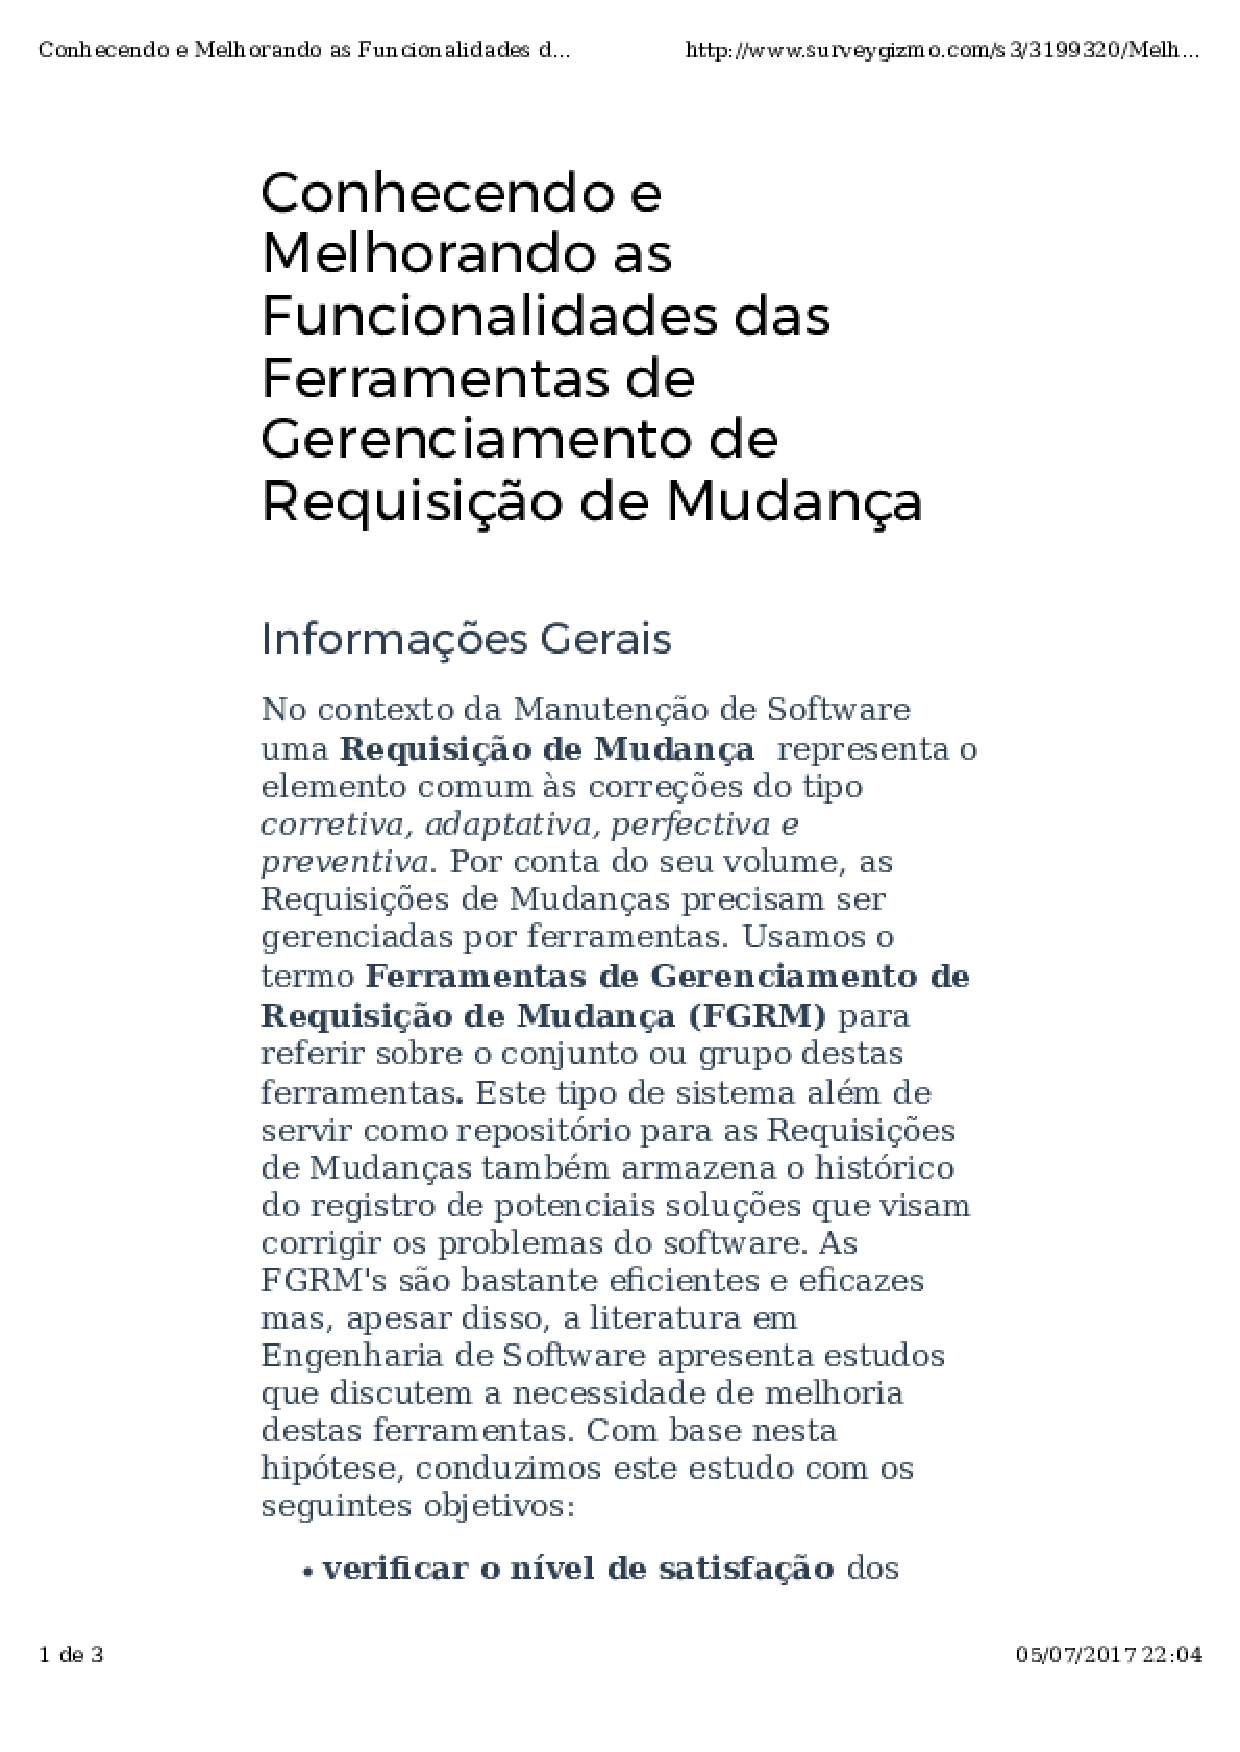
\includepdf[pages=-,scale=.8,linktodoc=true]{./apendices/img/form-melhorias-funcionalidades.pdf}

\chapter{Lista de Projetos Avaliação Sugestões de Melhorias}
\label{ch:app-tb-lista-projetos-sug-melhorias}
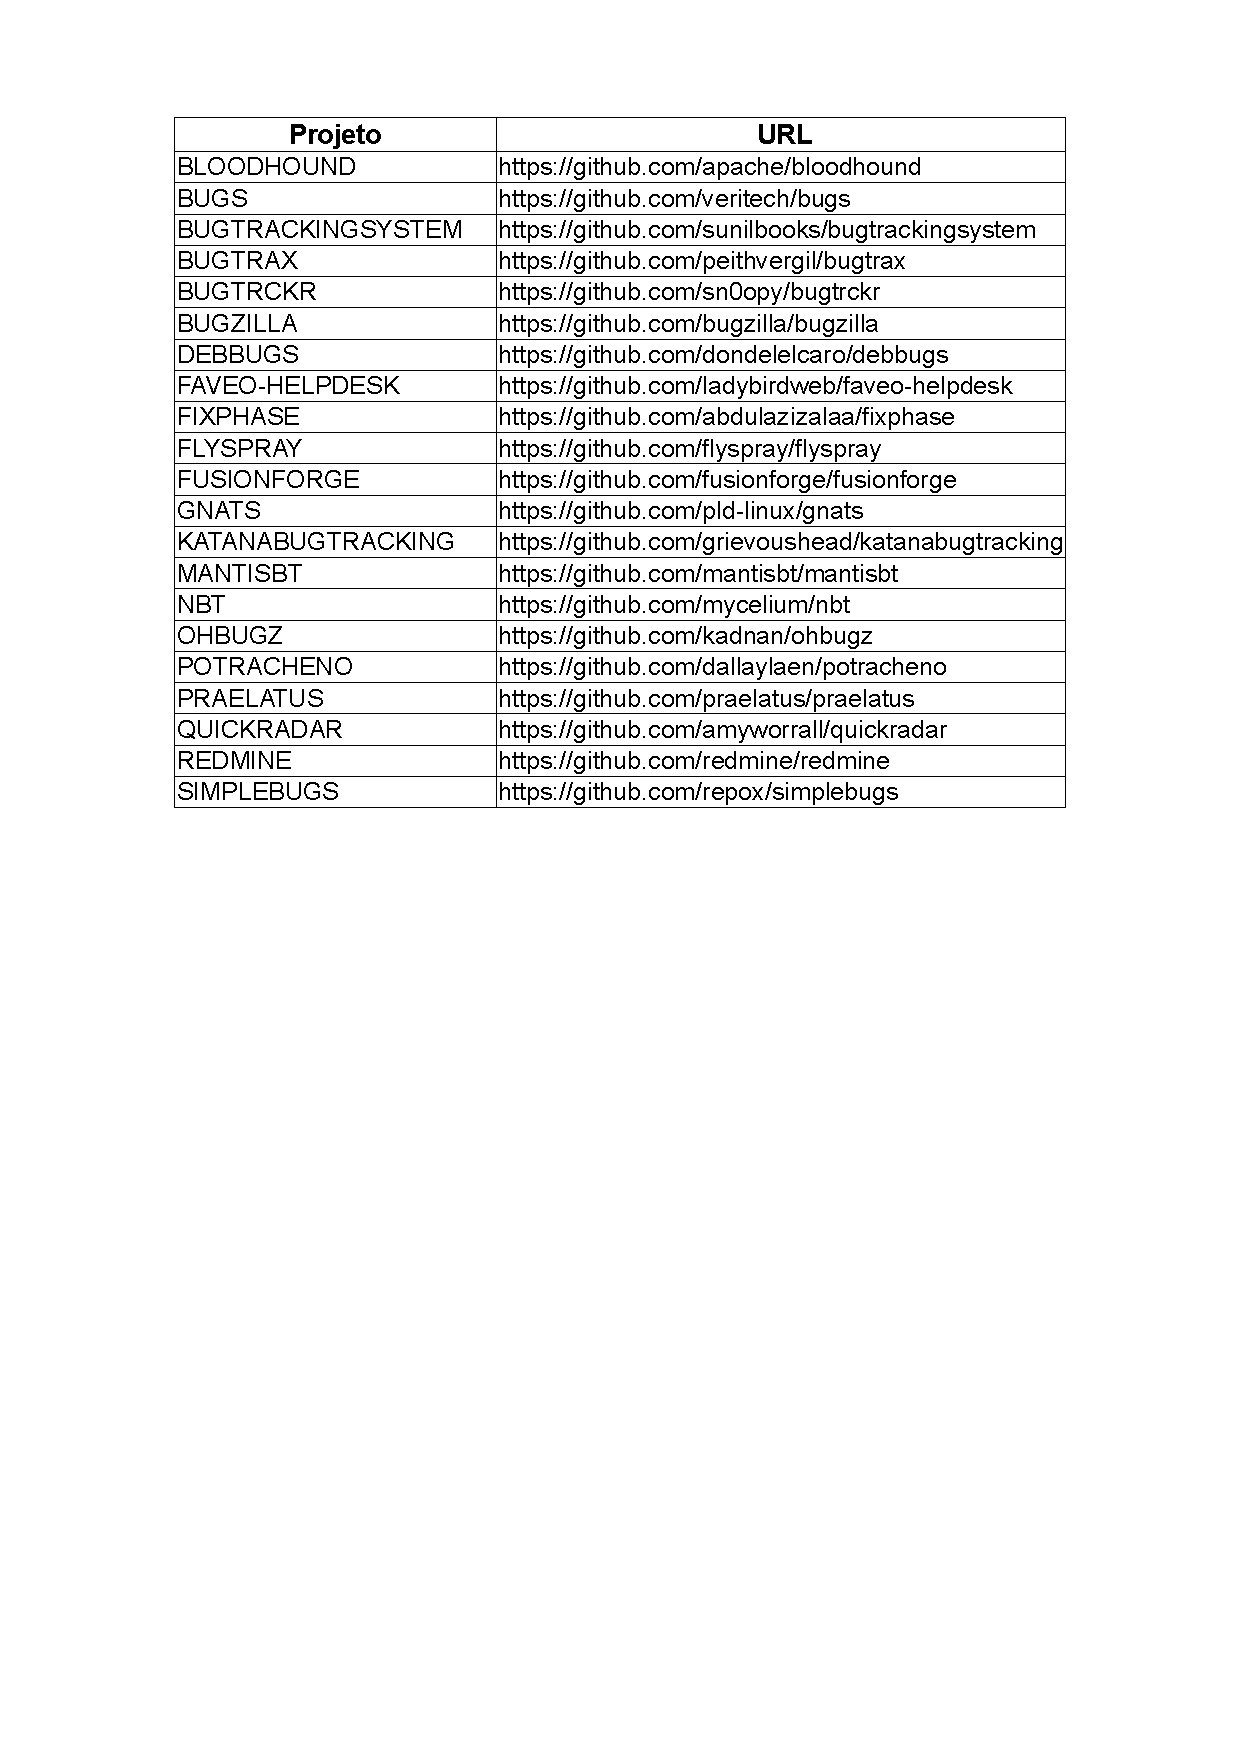
\includepdf[pages=-,scale=.8,linktodoc=true]{./apendices/img/tb-lista-projetos-avaliacao-sug-melhorias.pdf}

\chapter{Formulário Aplicado para Avaliação das Sugestões de Melhorias}
\label{ch:app-form-sug-melhorias}
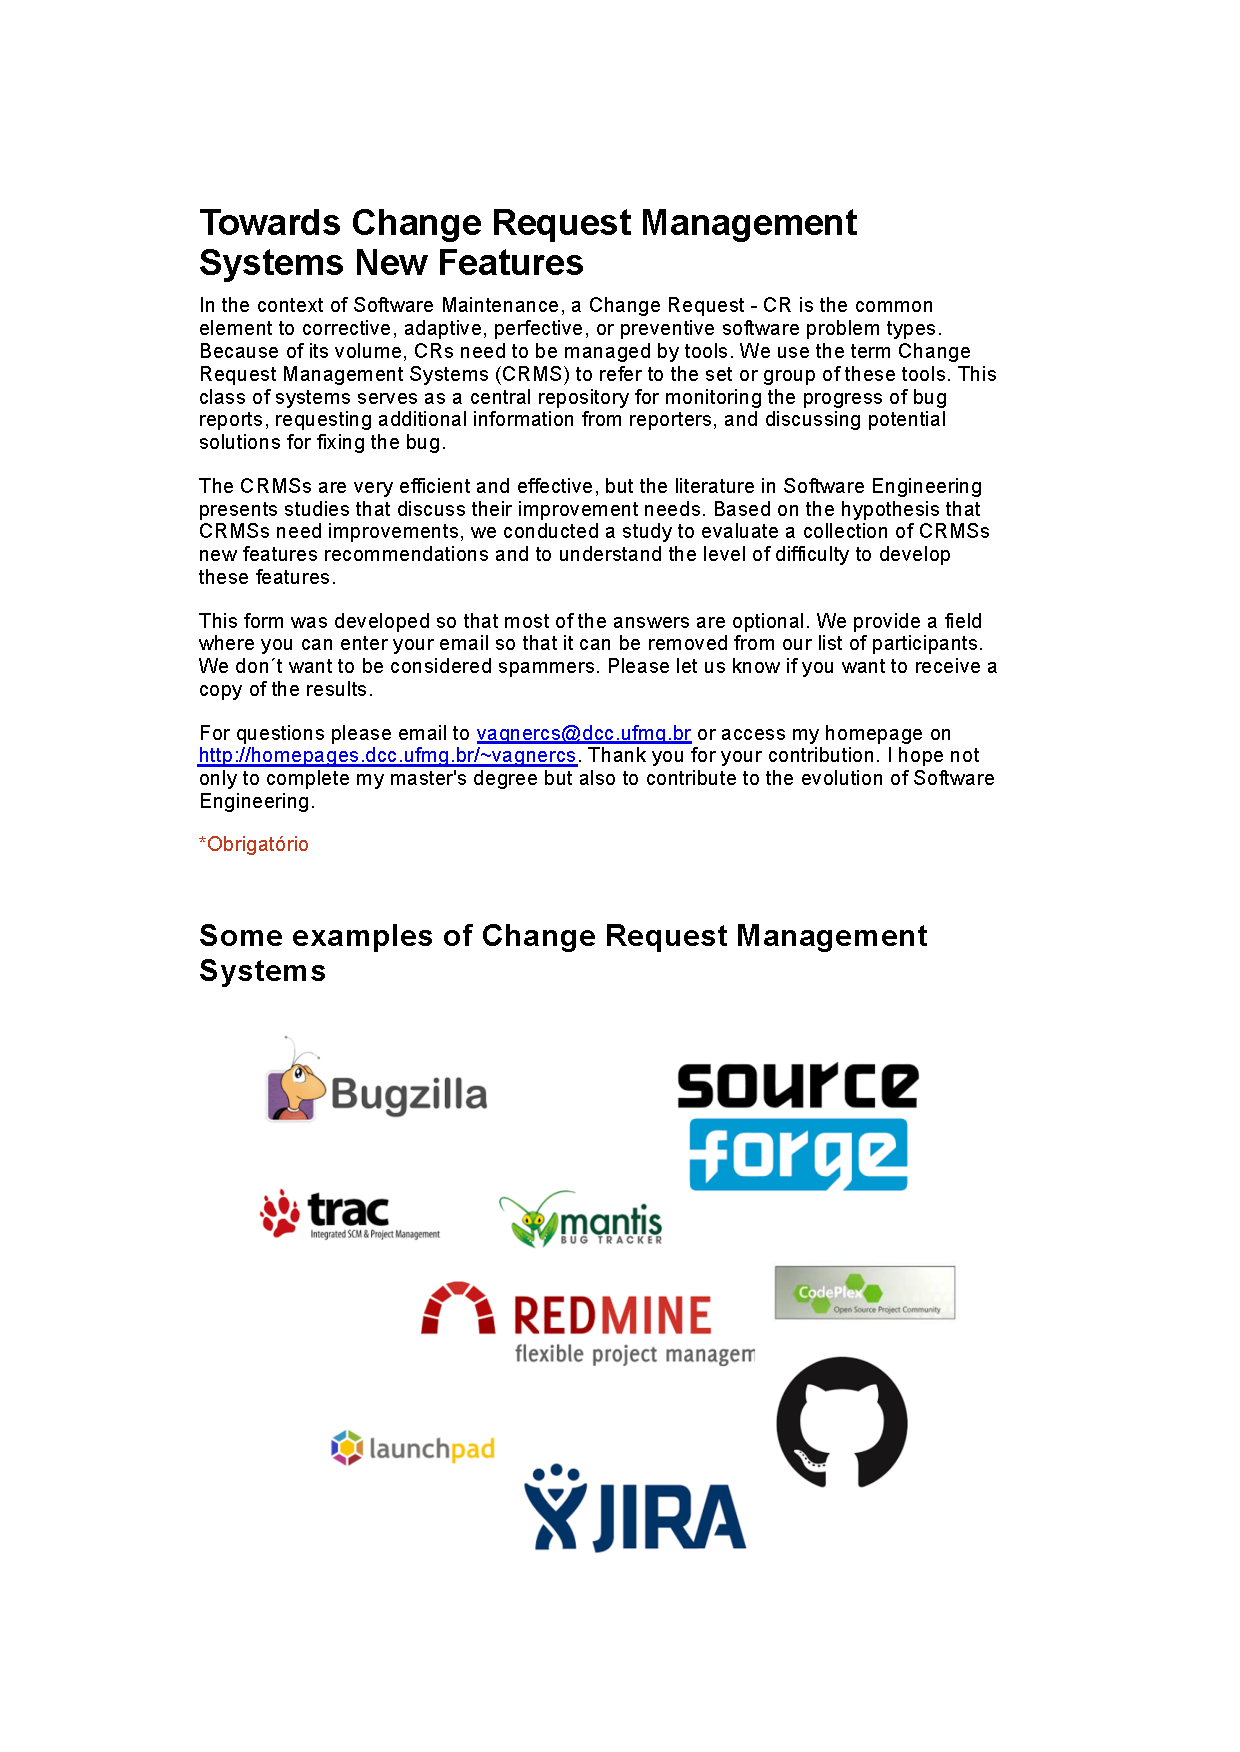
\includepdf[pages=-,scale=.8,linktodoc=true]{./apendices/img/form-sugestoes-melhorias.pdf}

\end{appendices}

\end{document}
